\documentclass[a4paper,UKenglish,cleveref,autoref,thm-restate]{lipics-v2021}
\usepackage{tikz}
\usetikzlibrary{intersections, calc, arrows, automata, positioning}
\newcommand{\fin}{{\mathit{fi}}}
\newcommand{\inn}{{\mathit{in}}}
%% Tikz
\RequirePackage{tikz}
\usetikzlibrary{arrows,snakes}

%\usepackage{caption}
\usepackage{subcaption}
\usepackage{graphicx}

\usepackage{pgf, verbatim}
\usetikzlibrary{arrows,automata}

\newcommand{\m}{{\sf m}}

\usepackage[linesnumbered,ruled]{algorithm2e}
\usepackage{amsmath}
\allowdisplaybreaks

\usepackage{floatrow}
% Table float box with bottom caption, box width adjusted to content
\newfloatcommand{capbtabbox}{table}[][\FBwidth]
\usepackage{tabularx}


\usepackage{xcolor,colortbl}
\usepackage{longtable}

\usepackage[font=small,labelfont=bf]{caption}


\usepackage{mathtools}
\usepackage{amssymb}
\usepackage{stmaryrd}
%\usepackage{mathabx}


\usepackage{amsthm}

%\theoremstyle{theorem}
%\newtheorem{theorem}{Theorem}[section]

%\theoremstyle{definition}
%\newtheorem{definition}[theorem]{Definition}%[section]

%\theoremstyle{proposition}
%\newtheorem{proposition}[theorem]{Proposition}%[section]

%\theoremstyle{lemma}
%\newtheorem{lemma}[theorem]{Lemma}%[section]

%\theoremstyle{corollary}
%\newtheorem{corollary}[theorem]{Corollary}%[section]

%\theoremstyle{example}
%\newtheorem{example}[theorem]{Example}%[section]

\newcommand{\commenteq}[1]{\hspace{2em} [\mbox{#1}]}

\newcommand{\suchthat}{:}%{\;\ifnum\currentgrouptype=16 \middle\fi|\;}

\usepackage[capitalise]{cleveref}


% change codes of < and >
\mathcode`<="4268
\mathcode`>="5269
\mathchardef\gr="213E
\mathchardef\ls="213C
\newcommand{\epsilonSim}{\stackrel{\epsilon}{\sim}}
\newcommand{\Dist}{\mathrm{Distr}}
\newcommand{\SubDist}{\mathrm{SubDistr}}
\newcommand{\support}{\mathrm{support}}
\newcommand{\lifting}[1]{\mathord{#1\!\!\uparrow}}
\newcommand{\nat}{\mathbb{N}}
\newcommand{\integer}{\mathbb{Z}}
\newcommand{\tv}{\mathit{tv}}

\newcommand{\glob}{\mathit{global}}
%\newcommand{\Pr}{\mathit{Pr}}
\newcommand{\local}{\mathit{local}}

\newcommand{\nxt}{\mathit{next}}
\newcommand{\M}{\mathcal{M}}
\newcommand{\pb}{\mathit{pb}}
\newcommand{\Hyp}{\mathcal{M}'}%\mathcal{M}_{\epsilon} {\widetilde{\mathcal{M}}}%
\newcommand{\errorParam}{\epsilon_2}%{\widetilde{\mathcal{M}}}%
\newcommand{\tauHyp}{\tau_{\epsilon}}
\newcommand{\R}{\mathcal{R}}
\newcommand{\Q}{\mathcal{Q}}

\newcommand{\adjust}{\mathit{adjust}}

\definecolor{OliveGreen}{rgb}{0,0.6,0}
\newcommand{\QT}[1]{{\color{OliveGreen}[#1]}}
 \newcommand{\cancel}[1]{{\color{gray}#1}}
 \newcommand{\modify}[1]{{\color{black}#1}}

 %%%%%%%%%%%%%%%%%%%%%%%%%%%%%%%%%%%%%%%%%%%%%%%%%%%%%%%%%%%%%%%%%%%%%%%%%%%%%%%%
 \bibliographystyle{plainurl}% the mandatory bibstyle

 \title{Approximate Bisimulation Minimisation} %TODO Please add

 %\titlerunning{} %TODO optional, please use if title is longer than one line

\author{Stefan Kiefer}{Department of Computer Science, University of Oxford, UK}{stekie@cs.ox.ac.uk}{https://orcid.org/0000-0003-4173-6877}{Supported by a Royal Society University Fellowship.}%TODO mandatory, please use full name; only 1 author per \author macro; first two parameters are mandatory, other parameters can be empty. Please provide at least the name of the affiliation and the country. The full address is optional

\author{Qiyi Tang}{Department of Computer Science, University of Oxford, UK}{qiyi.tang@cs.ox.ac.uk}{https://orcid.org/0000-0002-9265-3011}{}

\authorrunning{S.\ Kiefer and Q.\ Tang}%TODO mandatory. First: Use abbreviated first/middle names. Second (only in severe cases): Use first author plus 'et al.'

\Copyright{Stefan Kiefer and Qiyi Tang} %TODO mandatory, please use full first names. LIPIcs license is "CC-BY";  http://creativecommons.org/licenses/by/3.0/

 \ccsdesc{Theory of computation~Program verification}
 \ccsdesc{Theory of computation~Models of computation}
 \ccsdesc{Mathematics of computing~Probability and statistics} %TODO mandatory: Please choose ACM 2012 classifications from https://dl.acm.org/ccs/ccs_flat.cfm

 \keywords{Markov chains, Behavioural metrics, Bisimulation} %TODO mandatory; please add comma-separated list of keywords

 \category{} %optional, e.g. invited paper

\relatedversion{The paper is accepted to FSTTCS 2021.}
%\relatedversion{} %optional, e.g. full version hosted on arXiv, HAL, or other respository/website
 %\relatedversiondetails[linktext={opt. text shown instead of the URL}, cite=DBLP:books/mk/GrayR93]{Classification (e.g. Full Version, Extended Version, Previous Version}{URL to related version} %linktext and cite are optional

 %\supplement{}%optional, e.g. related research data, source code, ... hosted on a repository like zenodo, figshare, GitHub, ...
 %\supplementdetails[linktext={opt. text shown instead of the URL}, cite=DBLP:books/mk/GrayR93, subcategory={Description, Subcategory}, swhid={Software Heritage Identifier}]{General Classification (e.g. Software, Dataset, Model, ...)}{URL to related version} %linktext, cite, and subcategory are optional

 %\funding{(Optional) general funding statement \dots}%optional, to capture a funding statement, which applies to all authors. Please enter author specific funding statements as fifth argument of the \author macro.

\acknowledgements{We thank the anonymous reviewers of this paper for their constructive feedback.}%optional
%\acknowledgements{I want to thank \dots}%optional

\nolinenumbers %uncomment to disable line numbering

 %\hideLIPIcs  %uncomment to remove references to LIPIcs series (logo, DOI, ...), e.g. when preparing a pre-final version to be uploaded to arXiv or another public repository

 %Editor-only macros:: begin (do not touch as author)%%%%%%%%%%%%%%%%%%%%%%%%%%%%%%%%%%
\EventEditors{Miko{\l}aj Boja\'{n}czyk and Chandra Chekuri}
\EventNoEds{2}
\EventLongTitle{41st IARCS Annual Conference on Foundations of Software Technology and Theoretical Computer Science (FSTTCS 2021)}
\EventShortTitle{FSTTCS 2021}
\EventAcronym{FSTTCS}
\EventYear{2021}
\EventDate{December 15--17, 2021}
\EventLocation{Virtual Conference}
\EventLogo{}
\SeriesVolume{213}
\ArticleNo{28}
 %%%%%%%%%%%%%%%%%%%%%%%%%%%%%%%%%%%%%%%%%%%%%%%%%%%%%%

\begin{document}\sloppy
	
\maketitle
	
%TODO mandatory: add short abstract of the document
\begin{abstract}
We propose polynomial-time algorithms to minimise labelled Markov chains whose transition probabilities are not known exactly, have been perturbed, or can only be obtained by sampling.
Our algorithms are based on a new notion of an approximate bisimulation quotient, obtained by lumping together states that are exactly bisimilar in a slightly perturbed system.
We present experiments that show that our algorithms are able to recover the structure of the bisimulation quotient of the unperturbed system.
\end{abstract}
	
Reinforcement learning has achieved great success in areas such as Game-playing \citep{silver2018general,vinyals2019grandmaster}, robotics \cite{kober2013reinforcement}, large language models \citep{ouyang2022training}, etc.
However, due to safety concerns or physical limitations, in some real-world reinforcement learning problems, we must consider additional constraints that may influence the optimal policy and the learning process \citep{garcia2015comprehensive}.
% For example, a robotic arm must not take actions that may cause harm to itself or the environments.
A standard framework to handle such cases is the constrained Markov Decision Process (CMDP) \citep{altman1999constrained}.
Within the CMDP framework, the agent has to maximize
the expected cumulative reward while
obeying a finite number of constraints, which are usually in the form of expected cumulative cost criteria.

However, we are sometimes concerned with the problem with a continuum of constraints.
For example,
the constraints we meet might be time-evolving or subject to uncertain parameters, which
cannot be formulated as an ordinary CMDP
(see Examples \ref{Example_Time_Evolving} and  \ref{Example_Uncertain}).
In this paper we would study a generalized CMDP  
to address the above problem.  Because the constraints are not only infinite-number but also lie
in a continuous set,
the generalization is not trivial. Fortunately, we find that we can borrow the idea behind semi-infinite programming (SIP) \citep{remez1934determination, hettich1993semi} to deal with the semi-infinite constraints.
Accordingly, we propose \emph{semi-infinitely constrained Markov decision processes} (SICMDPs)
as a novel complement to the ordinary CMDP framework.
%More specifically,  an SICMDP model %, we consider 
%contains a continuum of constraints whereas an ordinary CMDP contains a finite number of constraints. 

%This generalization is natural but not trivial. However, we can brows the idea  
%The idea is quite natural and can be backtracked
%to the practice of extending linear programming to linear semi-infinite programming (LSIP) %\cite{remez1934determination, GobernaLSIO1998}.
%In addition, 
%As a complementary approach to the ordinary CMDP framework, 
%SICMDP can be used to model these problems  which cannot be described by a finite number of constraints
%that are not covered by .
%For example,
%the restrictions we consider can be time-evolving or subject to uncertain parameters
%, thus
%cannot be described by a finite number of constraints but a continuum of constraints 
%(see Examples \ref{Example_Time_Evolving} and  \ref{Example_Uncertain}).

We also present two reinforcement learning algorithms to solve SICMDPs called SI-CRL and SI-CPO, respectively.
SI-CRL is a model-based reinforcement learning algorithm designed for tabular cases, and SI-CPO is a policy optimization algorithm for non-tabular cases.
% and analyze its performance both theoretically and empirically.
The main challenge is that we need to deal with a continuum of constraints, thus reinforcement learning algorithms for ordinary CMDPs do not work anymore.
In SI-CRL, we tackle this difficulty by first transforming the reinforcement learning problem to an equivalent LSIP problem, which can then be solved using methods in the LSIP literature like the dual exchange methods \citep{Hu1990,reemtsen1998numerical}.
In SI-CPO, we resort to the idea of cooperative stochastic approximation developed in \cite{lan2020algorithms, wei2020comirror}.
As far as we know, we are the first to introduce tools from semi-infinitely programming (SIP) into the reinforcement learning community for solving constrained reinforcement learning problems.

% To the best of our knowledge, we are the first to apply tools from semi-infinitely programming (SIP) to solve reinforcement learning problems.
Furthermore, we give theoretical analysis for both SI-CRL and SI-CPO.
We decompose the error of SI-CRL into two parts: the statistical error from approximating the true SICMDP with an offline dataset and the optimization error due to the fact that the solution of the LSIP problem obtained by the dual exchange method is inexact.
On the optimization side, we show that the iteration complexity of SI-CRL is $O\left(\left\{\mathrm{diam}(Y)L\sqrt{|\gS|^2|\gA|m}/\left[(1-\gamma)\epsilon\right]\right\}^m\right)$.
On the statistical side, we show that the sample complexity of SI-CRL is $\widetilde O\left(\frac{|S|^2|A|^2}{\epsilon^2(1-\gamma)^3}\right)$ if the offline dataset is generated by a generative model, and $\widetilde O\left(\frac{|S||A|}{\nu_{\min} \epsilon^2(1-\gamma)^3}\right)$ if the dataset is generated by a probability measure $\nu$ as considered in \cite{chen2019information}.
Here $\widetilde O$ means that all logarithm terms are discarded.
For SI-CPO, things become a little more complicated because other than the statistical error and the optimization error, we also need to consider the function approximation error, which comes from imperfect policy parametrizations.
It is shown if the function approximation error can be controlled to $O(\epsilon)$ order, the iteration complexity of SI-CPO is $\widetilde{O}\left(\frac{1}{\epsilon^2(1-\gamma)^6}\right)$ and the sample complexity of SI-CPO is $\widetilde{O}(\frac{1}{\epsilon^4(1-\gamma)^{10}})$.
Here our iteration complexity bound is equivalent to a typical $\widetilde O(1/\sqrt{T})$ global convergence rate.

We perform a set of numerical experiments to illustrate the SICMDP model and validate our proposed algorithms.
Specifically, we examine two numerical examples, namely the discharge of sewage and ship route planning.
Through the discharge of sewage example, we show the advantage of the SICMDP framework over the CMDP baseline obtained by naive discretization in modeling realistic sequential decision-making problems.
Moreover, we demonstrate the effectiveness of the SI-CRL and SI-CPO algorithms in such tabular environments. 
In the ship route planning example, we illustrate the benefits of the SICMDP framework and the ability of the SI-CPO algorithm to address complex continuous control tasks involving continuous state spaces with modern deep reinforcement learning techniques.

% In summary, our contributions are listed as follows.
% First, we present the SICMDP model, which can be viewed as a generalization of the ordinary CMDP model.
% Second, we propose an algorithm to perform reinforcement learning for SICMDPs, which is called SI-CRL, and we believe that we are the first to apply tools from SIP
% to solve reinforcement learning problems.
% Third, we give a theoretical analysis of SI-CRL and identify both its sample complexity and iteration complexity.
% In addition, we perform numerical experiments to illustrate the SICMDP model and validate the SI-CRL algorithm.
% \{This paragraph can be removed!!! \}





\section{Preliminaries}
\label{section:preliminaries}
%quotient

We write $\nat$ for the set of nonnegative integers and $\integer^{+}$ for the set of positive integers. We write $\mathbb{R}$ for the set of real numbers. Let $S$ be a finite set. We denote by $\Dist(S)$ the set of probability distributions on~$S$. By default we view vectors, i.e., elements of $\mathbb{R}^{S}$, as row vectors. For a vector $\mu \in\mathbb{R}^{S}$ we write \modify{$\|\mu\|_1 := \sum_{s \in S} |\mu(s)|$ for its $L_1$-norm. A vector $\mu \in [0, 1]^{S}$ is a distribution (resp. subdistribution) over $S$ if $\|\mu\|_1 = 1$ (resp.  $0 \ls \|\mu\|_1 \le 1$).} For a (sub)distribution $\mu$ we write $\support(\mu) = \{s \in S \suchthat \mu(s) \gr 0 \}$ for its support. %For a relation $R \subseteq S \times S$, we write $R^{-1}$ as the converse relation of $R$. %We denote column vectors by boldface letters; in particular, $\one \in \{1\}^{S}$ and  $\zero \in \{0\}^{S}$ are column vectors all whose entries are $1$ and $0$, respectively. For $s \in S$ we write $\delta_s$ for the (Dirac) distribution over $S$ with $\delta_{s}(s) = 1$ and $\delta_{s}(r) = 0$ for $r \in S \setminus \{s\}$.

 %total variation distance
%Given two distributions $\mu \in \Dist(S)$ and $\nu \in \Dist(S)$, the \emph{total variation distance} between $\mu$ and $\nu$ is defined as follows: $d_{\tv}(\mu, \nu) = \sup_{E \subseteq S } |\mu(E) - \nu(E)| = \frac{1}{2} |\mu - \nu|$.

A partition of the states $S$ is a set $X$ consisting of pairwise disjoint subsets $E$ of $S$ with $\bigcup_{E \in X} = S$. For an equivalence relation $\R \subseteq S \times S$, $S /_{\R}$ denotes its quotient set and $[s]_\R$ denotes the $\R$-equivalence class of $s \in S$.

%LMC definition
A \emph{labelled Markov chain} (LMC) is a quadruple $<S, L, \tau, \ell>$ consisting of a nonempty finite set $S$ of states, a nonempty finite set $L$ of labels, a transition function $\tau : S \to \Dist(S)$, and a labelling function $\ell: S \to L$.

We denote by $\tau(s)(t)$ the transition probability from $s$ to $t$. Similarly, we denote by $\tau(s)(E) = \sum_{t \in E} \tau(s)(t)$ the transition probability from $s$ to $E \subseteq S$.
For the remainder of the paper,  we fix an LMC $\M = <S,  L, \tau, \ell>$. Let $|\M|$ denote the number of states, $|S|$.

% direct sum of two LMCs
The direct sum $\M_1 \oplus \M_2$ of two LMCs $\M_1 = <S_1, L_1, \tau_1, \ell_1>$ and $\M_2 = <S_2, L_2, \tau_2, \ell_2>$ is the LMC formed by combining the state spaces of $\M_1$ and $\M_2$.

% probabilistic bisimulation and probabilistic bisimilarity distances
An equivalence relation $\R \subseteq S \times S$ is a \emph{probabilistic bisimulation} if for all $(s, t) \in \R$, $\ell(s) = \ell(t)$ and
$\tau(s)(E) = \tau(t)(E)$ for each $\R$-equivalence class $E$. \emph{Probabilistic bisimilarity}, denoted by $\mathord{\sim_{\M}}$ (or $\mathord{\sim}$ when $\M$ is clear), is the largest probabilistic bisimulation.

Any probabilistic bisimulation $\R$ on $\M$ induces a quotient LMC denoted by $\M/_{\R} = <S/_{\R}, L, \tau/_{\R}, \ell/_{\R}>$ where the transition function $\tau/_{\R}([s]_{\R})([t]_{\R}) = \tau(s)([t]_{\R})$ and the labelling function $\ell/_{\R}([s]_\R) = \ell(s)$.

We define the notion of an \emph{approximate quotient}.  Let $\epsilon \ge 0$. An LMC $\Q$ is an \emph{$\epsilon$-quotient} of $\M$ if and only if there is transition function $\tau': S \to \Dist(S)$ such that for all $s \in S$ we have $\|\tau'(s) - \tau(s)\|_1 \le \epsilon$ and $\Q$ is the (exact) bisimulation quotient of the LMC $\M' = <S, L, \tau',\ell>$, that is, $\Q = \M'/_{\sim_{\M'}} $. Since the choice of $\tau'$ is not unique, there might be multiple $\epsilon$-quotients of $\M$. We are interested in the problem of obtaining an $\epsilon$-quotient of $\M$ with small state space. We retrieve the notion of (exact) quotient when $\epsilon = 0$. For $s$ from $\M$, denote the state in $\Q$ which corresponds to $s$ by $[s]^{\epsilon}_{\Q}$ (or $[s]^{\epsilon}$ when $\Q$ is clear).
%\item
%for any $s' \in S'$ and $s \in f^{-1}(s')$ we have $\ell'(s') = \ell(s)$;
%The pseudometric \emph{probabilistic bisimilarity distance} of Desharnais et al. \cite{DGJP1999} , which we denote by $d_{\pb}$, is a function from $S \times S$ to $[0, 1]$, that is, an element of $[0, 1]^{S \times S}$. It can be defined as the least fixed point of the following function:
%\[
%\Delta(d)(s, t) = \left \{
%\begin{array}{ll}
%1 & \mbox{if $\ell(s) \not= \ell(t)$}\\
%\displaystyle \min_{\omega \in \Omega(\tau(s), \tau(t))} \sum_{u, v \in S} \omega(u, v) \; d(u, v) & \mbox{otherwise}
%\end{array}
%\right .
%\]
%12

The set $\Omega(\mu, \nu)$ of \emph{couplings} of $\mu,\nu \in \Dist(S)$ is defined as $\Omega(\mu, \nu)=\left \{ \, \omega \in \Dist(S \times S) \suchthat \sum_{t \in S} \omega(s, t) = \mu(s) \wedge \sum_{s \in S} \omega(s, t) = \nu(t) \, \right \}$. Note that a coupling $\omega \in \Omega$ is a joint probability distribution with marginals $\mu$ and $\nu$ (see, e.g., \cite[page 260-262]{billingsley1995}).

%For all $s,t \in S$, $s \sim t$ if and only if $d_{\pb}(s,t) = 0$ \cite[Theorem~1]{DGJP1999}.

%quotient LMC  an LMC $\M = <S, L, \tau, \ell>$


%distances
%epsilon-bisimulation
%\begin{definition}
%	\label{definition:epsilon-lifting}
	The \emph{$\epsilon$-lifting} of a relation $\R\subseteq S \times S$ proposed by Tracol et al.~\cite{TracolDesharnaisZhioua2011} is the relation $\lifting{\R}_{\epsilon} \subseteq \Dist(S) \times \Dist(S)$ defined by $(\mu, \nu) \in \lifting{\R}_{\epsilon}$ if there exists $\omega \in \Omega(\mu, \nu)$ such that $\sum_{ (u,v) \in \R} \omega(u, v) \ge 1 - \epsilon$.
%\end{definition}

%(Desharnais et al.)
The \emph{$\epsilon$-bisimulation} ($\sim_{\epsilon}$) by Desharnais et al.~\cite{DesharnaisLavoletteTracol2008} is a relation $\R \subseteq S \times S$ in which for all $(s, t) \in \R$ we have  $\ell(s) = \ell(t)$ and $(\tau(s), \tau(t)) \in \lifting{\R}_{\epsilon}$. The $\epsilon$-bisimulation is reflexive and symmetric, but in general not transitive; hence, it is not an equivalence relation.
%\begin{itemize}
%	\item
%	$\ell(s) = \ell(t)$, and
%	\item  $(\tau(s), \tau(t)) \in \lifting{\mathcal{R}}_{\epsilon}$.
%\end{itemize}

%global epsilon bisimulation
%Given an LMC $\M_1 = <S_1, L, \tau_1, \ell_{1}>$ and $\M_2 = <S_2, L, \tau_2, \ell_2>$.

\section{Properties of Approximate Quotients}
\label{section:approximate-quotient-properties}

\begin{figure}[h]
	\centering
	
	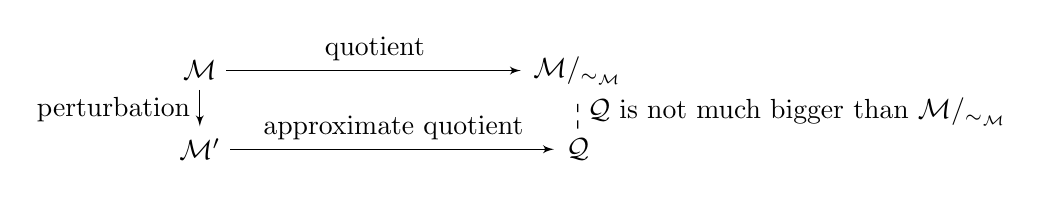
\begin{tikzpicture}[xscale=.6,>=latex',shorten >=1pt,node distance=3cm,on grid,auto]
	
	\node[label] (M) at (0,0) {$\M$};
	\node[label] (MQ) at (8,0) {$\M /_{\sim_{\M}}$};
	\node[label] (Me) at (0,-1) {$\Hyp$};
	\node[label] (MeQ) at (8,-1) {$\Q$};
	
	\path[->] (M) edge node [midway, above] {quotient} (MQ);
	\path[->] (M) edge node [midway, left] {perturbation} (Me);
	\path[->] (Me) edge node [midway, above] {approximate quotient} (MeQ);		
	\path[dashed] (MeQ) edge node [midway, right] {$\Q$ is not much bigger than $\M /_{\sim_{\M}}$} (MQ);		
	%\path[->] (Meq) edge node [midway, below] {minimisation} (MOut);				
	\end{tikzpicture}
	\caption{Problem setup.}\label{fig:problem-setup}
\end{figure}
%NP-hard to obtain minimum approximate quotient

Recall from the introduction that we are given an LMC $\Hyp$, which is a slightly perturbed version of an (unknown) LMC $\M$. By slightly perturbed we mean that for each state the successor distributions in $\Hyp$ and~$\M$ have small (say, less than~$\epsilon$) $L_1$-distance. For example, with sampling we can obtain with high probability a perturbed system that has small distance with $\M$. Assume there are many symmetries, that is, lots of probabilistic bisimilar states in $\M$. The state space of $\M$ can then be compressed a lot by (exact) quotienting. Since the transition probabilities are perturbed in $\Hyp$, the states that are probabilistic bisimilar in $\M$ might become inequivalent in $\Hyp$; as a result, the (exact) bisimulation quotient of $\Hyp$ is much larger than that of $\M$. Given a small compression parameter $\errorParam \gr 0$, we aim to compute an approximate quotient $\Q$, an $\epsilon'$-quotient of $\Hyp$ that satisfies two conditions: \modify{(1) $\epsilon'$ should be small, so that little precision is
sacrificed; and (2) the state space of the quotient should be small, to speed up
verification algorithms. Our contribution consists of approximate quotienting algorithms with (a) theoretical guarantees on goal (1) in \cref{theorem:bounding-global-distance} and
\cref{corollary:bounding-quotient-error}, applying to both algorithms: $\epsilon'$ is bounded (and can be controlled) by a compression parameter $\epsilon_2$ and
the number of iterations $i$; (b) empirical results on goal (2): the experiments show that our algorithms produce small quotients.} %(1) $\epsilon'$ is not much bigger than $\errorParam$; and (2) $\Q$ is not much bigger than $\M/_{\sim_{\M}}$, the quotient of $\M$. \cref{fig:problem-setup} shows the setup of our problem.

We first show that it is hard to find an $\errorParam$-quotient of $\Hyp$ with minimum number of states: $\Q^{*}= \arg\min\{|\Q| : \Q \text{ is an } \errorParam\text{-quotient of }\Hyp\}.$ If there are several $\errorParam$-quotients of $\Hyp$ of minimum size, $\Q^{*}$ can be taken to be any one of them. Unfortunately, this problem is unlikely to have an efficient (polynomial-time) solution, as we will see from the next theorem that the decision version of this problem is $\sf NP$-complete.


\begin{figure}[h]
	\begin{minipage}{0.45\linewidth}
		\centering
		
		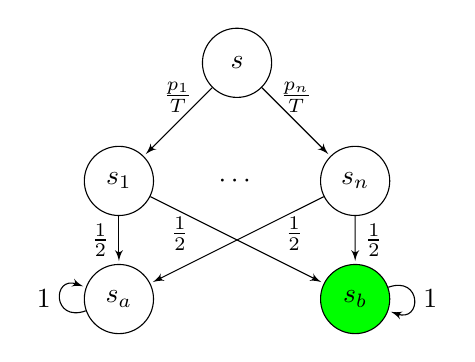
\begin{tikzpicture}[xscale=.6,>=latex',shorten >=1pt,node distance=3cm,on grid,auto]
		
		\node[state] (us) at (3,4) {$s$};
		\node[state] (u1) at (0.5,2.5) {$s_{1}$};
		\node[label] at (3,2.5) {$\cdots$};
		\node[state] (un) at (5.5,2.5) {$s_{n}$};
		
		
		\node[state] (qb) at (0.5,1) {$s_a$};
		\node[state, fill=green] (qc) at (5.5,1) {$s_b$};
		
		\path[->] (us) edge node  [midway,above] {$\frac{p_1}{T}$} (u1);
		\path[->] (us) edge node  [midway,above] {$\frac{p_n}{T}$} (un);
		
		
		\path[->] (qc) edge  [loop right] node [right] {$1$} (qc);
		\path[->] (qb) edge [loop left] node [left]{$1$} (qb);
		
		\path[->] (u1) edge node  [midway,left] {$\frac{1}{2}$} (qb);
		\path[->] (u1) edge node  [very near start, below,xshift=0.1cm] {$\frac{1}{2}$} (qc);
		\path[->] (un) edge node [very near start, below,xshift=-0.1cm] {$\frac{1}{2}$} (qb);
		\path[->] (un) edge node [midway,right] {$\frac{1}{2}$} (qc);
		
		\end{tikzpicture}
		
	\end{minipage}
	\hspace{0.5cm}
	\begin{minipage}{0.45\linewidth}
		\centering
		
		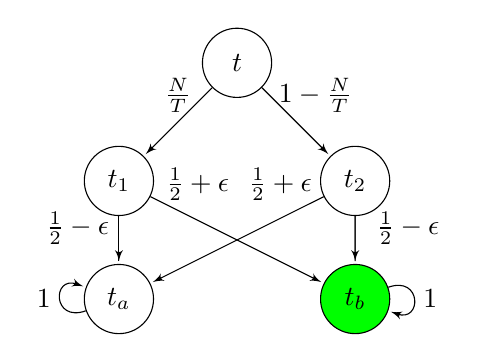
\begin{tikzpicture}[xscale=.6,>=latex',shorten >=1pt,node distance=3cm,on grid,auto]
		
		\node[state] (t) at (2,4) {$t$};
		
		\node[state] (t1) at (-0.5,2.5) {$t_1$};
		\node[state] (t2) at (4.5,2.5) {$t_2$};
		
		\node[state] (qb) at (-0.5,1) {$t_a$};
		\node[state, fill=green] (qc) at (4.5,1) {$t_b$};
		
		\path[->] (t) edge node [midway, above] {$\frac{N}{T}$} (t1);
		\path[->] (t) edge node [midway, above, xshift=0.25cm] {$1-\frac{N}{T}$} (t2);
		
		\path[-] (t1) edge node [midway, right] {} (qb);
		\path[->] (t1) edge node [near start, left] {$\frac{1}{2} - \epsilon$} (qb);
		\path[->] (t1) edge node [near start, above,xshift=0.05cm,yshift=0.1cm] {$\frac{1}{2} + \epsilon$} (qc);
		
		\path[-] (t2) edge node [midway, right] {} (qc);		
		\path[->] (t2) edge node [near start, above, yshift=0.1cm] {$\frac{1}{2}+ \epsilon$} (qb);
		\path[->] (t2) edge node [near start, right,xshift=0.15cm] {$\frac{1}{2} - \epsilon$} (qc);
		
		\path[->] (qc) edge [loop right] node [midway, right] {$1$} (qc);
		\path[->] (qb) edge [loop left]   node [midway, left]{$1$} (qb);
		
		\end{tikzpicture}
	\end{minipage}
	\caption{The LMC in the reduction for {\sf NP}-hardness. All states have the same label $a$ except $s_b$ and $t_b$ which have label $b$.
	}\label{fig:reductionfromSubsset}
\end{figure}

Given an LMC $\Hyp$, a compression parameter $\errorParam \gr 0$ and a constant $k \in \integer^{+}$, it is {\sf NP}-complete to decide whether there exists an $\errorParam$-quotient of $\Hyp$ of size $k$. The hardness result is by reduction from the Subset Sum problem. Given a set $P =\{p_1, \ldots, p_n\}$ and $N \in \nat$, Subset Sum asks whether there exists a set $Q \subseteq P$ such that $\sum_{p_i \in Q} p_i = N$. Given an instance of Subset Sum $<P, N>$ where $P =\{p_1, \ldots, p_n\}$ and $N \in \nat$, we construct an LMC; see \cref{fig:reductionfromSubsset}. Let $T = \sum_{p_i \in P} p_i$, $\epsilon = \frac{1}{2T}$ and $k = 5$. \modify{In the LMC, state $s$ transitions to state $s_i$ with probability $p_i / T$ for all $1 \le  i \le n$. Each state $s_i$ transitions to $s_a$ and $s_b$ with equal probabilities. State $t$ transitions to $t_1$ and $t_2$ with probability $N / T$ and $1 - N / T$, respectively. State $t_1$ (resp. $t_2$) transitions to $t_a$ (resp. $t_b$) and $t_b$ (resp. $t_a$) with probability $\frac{1}{2} - \epsilon$ and $\frac{1}{2} + \epsilon$, respectively. All the remaining states transition to the successor state with probability one. States $s_b$ and $t_b$ have label $b$ and all other states have label $a$.} We can show that $<P, N> \in {\mbox{Subset Sum}} \iff$ there exists an $\frac{1}{2T}$-quotient of $\Hyp$ of size $5$.

\begin{restatable}{theorem}{theoremMinimumApproximateQuotientNPComplete}\label{theorem: minimum-approximate-quotient-NP-complete}
	Given an LMC $\Hyp$, $\errorParam \in (0, 1]$ and $k \in \integer^{+}$. The problem whether there exists an $\errorParam$-quotient of $\Hyp$ of size $k$ is $\sf NP$-complete. It is $\sf NP$-hard even for (fixed) $k=5$.
\end{restatable}

Due to the $\sf NP$-hardness result, we hope to develop practical algorithms to compute approximate quotients of $\Hyp$ that are small but not necessarily of minimum size. To do that, an intuitive idea is to merge ``similar'' states. As we have discussed in the introduction, merging states with small probabilistic bisimilarity distances might be insufficient. Consider the LMC shown in \cref{fig:intro3}. Assume $\epsilon \gr 0$. The states $s_1$ and $t_1$ ($s_2$ and $t_2$) have probabilistic bisimilarity distance one. Thus, to merge $s_1$, $t_1$ or $s_2$, $t_2$, one needs to merge states with probabilistic bisimilarity distance one. Alternatively, we explore the relation of approximate quotient and $\epsilon$-bisimulation. It is not hard to prove the following proposition:%that if $\Q$ is an $\errorParam$-quotient of $\Hyp$, in the LMC $\Hyp \oplus \Q$, for all $s$ from $\Hyp$ we have $s \sim_{\frac{\errorParam}{2}} [s]^{\errorParam}$. %We will see later by examples that the idea of merging states with small approximate probabilistic bisimilar distances does not work.


\begin{restatable}{proposition}{propositionApproximateGlobalRelationSubset}\label{proposition:approximate-quotient-implies-approximate-bisimulation}
	Let $\Q$ be an $\errorParam$-quotient of $\Hyp$. Then in the LMC $\Hyp \oplus \Q$, we have $s \sim_{\frac{\errorParam}{2}} [s]^{\errorParam}_{\Q}$ for all $s$ from $\Hyp$.
\end{restatable}

\begin{figure}[t]
	\centering
	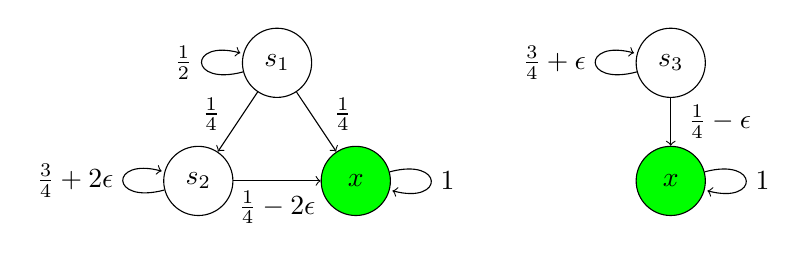
\begin{tikzpicture}
	\tikzstyle{BoxStyle} = [draw, circle, fill=black, scale=0.05,minimum width = 0.001pt, minimum height = 0.001pt]
	\node[state] (s) at (3,4) {$s_1$};
	\node[state] (s1) at (2,2.5) {$s_{2}$};
	\node[state, fill=green] (x) at (4,2.5) {$x$};
	\path[->] (s) edge [loop left] node  [midway,left] {$\frac{1}{2}$} (s);
	\path[->] (s) edge node  [midway,left,xshift=-0.1cm,yshift=0.1cm] {$\frac{1}{4}$} (s1);
	\path[->] (s) edge node  [midway,right,xshift=0.1cm,yshift=0.1cm] {$\frac{1}{4}$} (x);
	\path[->] (x) edge [loop right] node [midway, right] {$1$} (x);
	\path[->] (s1) edge node  [midway,below] {$\frac{1}{4}-2\epsilon$} (x);
	\path[->] (s1) edge [loop left] node [midway, left] {$\frac{3}{4} + 2\epsilon$} (s1);
	
	\node[state] (t) at (8,4) {$s_3$};
	\node[state, fill=green] (y) at (8,2.5) {$x$};
	\path[->] (t) edge [loop left] node  [midway,left] {$\frac{3}{4}+\epsilon$} (t);
	\path[->] (t) edge node  [midway,right,xshift=0.1cm] {$\frac{1}{4}-\epsilon$} (y);
	\path[->] (y) edge [loop right] node [midway, right] {$1$} (y);
	
	%	\node[state] (ss1) at (7,4) {$s_1$};
	%	\node[state, fill=green] (z) at (7,2.5) {$x$};
	%	\path[->] (ss1) edge [loop left] node  [midway,left] {$\frac{3}{4}+2\epsilon$} (ss1);
	%	\path[->] (ss1) edge node  [midway,right,xshift=0.1cm] {$\frac{1}{4}-2\epsilon$} (z);
	%	\path[->] (z) edge [loop right] node [midway, right] {$1$} (z);
	\end{tikzpicture}
	\caption{An LMC in which $s_1 \sim_{\epsilon} s_3 \sim_{\epsilon} s_2$.}
	\label{fig:exampleGlobal}
\end{figure}
\begin{figure}[t]
	\centering
	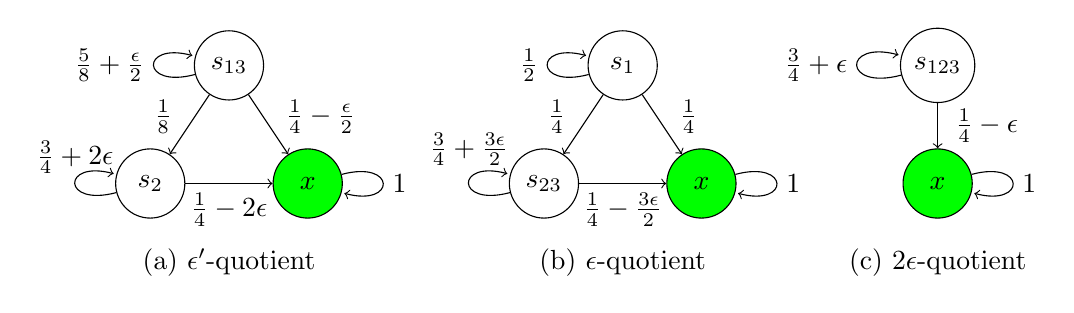
\begin{tikzpicture}
	\tikzstyle{BoxStyle} = [draw, circle, fill=black, scale=0.05,minimum width = 0.001pt, minimum height = 0.001pt]
	\node[state] (s) at (3,4) {$s_{13}$};
	\node[state] (s1) at (2,2.5) {$s_{2}$};
	\node[state, fill=green] (x) at (4,2.5) {$x$};
	\path[->] (s) edge [loop left] node  [midway,left] {$\frac{5}{8}+\frac{\epsilon}{2}$} (s);
	\path[->] (s) edge node  [midway,left,xshift=-0.1cm,yshift=0.1cm] {$\frac{1}{8}$} (s1);
	\path[->] (s) edge node  [midway,right,xshift=0.1cm,yshift=0.1cm] {$\frac{1}{4}-\frac{\epsilon}{2}$} (x);
	\path[->] (x) edge [loop right] node [midway, right] {$1$} (x);
	\path[->] (s1) edge node  [midway,below] {$\frac{1}{4}-2\epsilon$} (x);
	\path[->] (s1) edge [loop left] node [midway, above] {$\frac{3}{4} + 2\epsilon$} (s1);
	\node at (3, 1.5) {(a) $\epsilon'$-quotient};
	
	\node[state] (s) at (8,4) {$s_1$};
	\node[state] (s1) at (7,2.5) {$s_{23}$};
	\node[state, fill=green] (x) at (9,2.5) {$x$};
	\path[->] (s) edge [loop left] node  [midway,left] {$\frac{1}{2}$} (s);
	\path[->] (s) edge node  [midway,left,xshift=-0.1cm,yshift=0.1cm] {$\frac{1}{4}$} (s1);
	\path[->] (s) edge node  [midway,right,xshift=0.1cm,yshift=0.1cm] {$\frac{1}{4}$} (x);
	\path[->] (x) edge [loop right] node [midway, right] {$1$} (x);
	\path[->] (s1) edge node  [midway,below] {$\frac{1}{4}-\frac{3\epsilon}{2}$} (x);
	\path[->] (s1) edge [loop left] node [midway, above,yshift=0.1cm] {$\frac{3}{4} + \frac{3\epsilon}{2}$} (s1);	
	\node at (8, 1.5) {(b) $\epsilon$-quotient};
	
	\node[state] (t) at (12,4) {$s_{123}$};
	\node[state, fill=green] (y) at (12,2.5) {$x$};
	\path[->] (t) edge [loop left] node  [midway,left] {$\frac{3}{4}+\epsilon$} (t);
	\path[->] (t) edge node  [midway,right,xshift=0.1cm] {$\frac{1}{4}-\epsilon$} (y);
	\path[->] (y) edge [loop right] node [midway, right] {$1$} (y);
	\node at (12, 1.5) {(c) $2\epsilon$-quotient};	
	%	\node[state] (ss1) at (7,4) {$s_1$};
	%	\node[state, fill=green] (z) at (7,2.5) {$x$};
	%	\path[->] (ss1) edge [loop left] node  [midway,left] {$\frac{3}{4}+2\epsilon$} (ss1);
	%	\path[->] (ss1) edge node  [midway,right,xshift=0.1cm] {$\frac{1}{4}-2\epsilon$} (z);
	%	\path[->] (z) edge [loop right] node [midway, right] {$1$} (z);
	\end{tikzpicture}
	\caption{(a) An $\epsilon'$-quotient obtained by merging $s_1$ and $s_3$ where $\epsilon'$ is at least $\frac{1}{4}+\epsilon$; (b) An $\epsilon$-quotient obtained by merging $s_2$ and $s_3$; (b) A $2\epsilon$-quotient obtained by merging $s_1$, $s_2$ and $s_3$.}
	\label{fig:exampleMerge}
\end{figure}

\cref{proposition:approximate-quotient-implies-approximate-bisimulation} suggests that $\epsilon_2$-quotients and $\epsilon_2$-bisimulation are related.  The runtime of the algorithm to compute the $\epsilon_2$-bisimulation in \cite{DesharnaisLavoletteTracol2008} is $O(|S|^7)$ which makes it not practical for large systems. Furthermore, the algorithms based on merging states that are $\epsilon_2$-bisimilar may produce an $\epsilon'$-quotient where $\epsilon'$ is large, violating the first condition of a satisfying approximate quotient. Assume the positive number $\epsilon$ is much smaller than $\frac{1}{8}$. Let us choose the compression parameter $\epsilon_2$ to be the same as $\epsilon$. We compute the $\epsilon$-bisimulation of the LMC shown in \cref{fig:exampleGlobal} and get $s_1 \sim_{\epsilon} s_3 \sim_{\epsilon} s_2$.  Since $\epsilon$-bisimulation is not an equivalence relation, $s_1  \sim_{\epsilon} s_2$ does not necessarily follow. Indeed, in this LMC, we have $s_1  \sim_{2\epsilon} s_2$ but not $s_1  \sim_{\epsilon} s_2$. If $s_2$ and $s_3$, related by $\sim_{\epsilon}$, are chosen to be merged, the resulting LMC in \cref{fig:exampleMerge}(b) is an $\epsilon$-quotient. However, if $s_1$ and $s_3$ are (unfortunately) chosen to be merged, the resulting LMC, shown in \cref{fig:exampleMerge}(a), is an $\epsilon'$-quotient where $\epsilon'$ cannot be smaller than $\frac{1}{4}+\epsilon$. This $\epsilon'$, much bigger than $\epsilon$ under the assumption that $\epsilon$ is much smaller than $\frac{1}{8}$, makes the resulting LMC undesirable. This example shows that arbitrarily merging states that are $\epsilon$-bisimilar may not work. The LMC in \cref{fig:exampleMerge}(c) is obtained by merging $s_1$, $s_2$ and $s_3$, the states that are related by the transitive closure of $\sim_{\epsilon}$. We show in the appendix that for any $n \in \integer^{+}$ there exists an LMC $\M(n)$ such that merging all states in $\M(n)$  that are related by the transitive closure of $\sim_{\epsilon}$ results in an $\epsilon'$-quotient where $\epsilon'$ is at least $n\epsilon$.

%Since $s R_{\epsilon'} s_1$ does not hold for $\epsilon' \ls 2\epsilon$, we have $s R_{\epsilon'} t$ does not hold for $\epsilon' \ls 2\epsilon$, that is, $s \mathord{R_{\epsilon}} t$ does not hold. This implies that $\mathord{\sim_{\epsilon}} \not\subseteq \mathord{R_{\epsilon}}$. %Together with the previous proposition, we have $R_{\epsilon} \subset \sim_{\epsilon}$.



\cref{lemma:additivity-property}, the additivity lemma, asserts an additivity property of approximate quotients. In \cref{section:minimisation-algorithms}, this lemma will be applied as the two minimisation algorithms successively compute a sequence of approximate quotients.



%TODO parameter continuous

\begin{restatable}{lemma}{lemmaAdditivityProperty}\label{lemma:additivity-property}
		Consider three LMCs $\M_1$, $\M_2$ and $\M_3$. Let $\epsilon_1 \ge 0$ and $\M_2$ be an $\epsilon_1$-quotient of $\M_1$. Let $\epsilon_2 \ge 0$ and $\M_3$ be an $\epsilon_2$-quotient of $\M_2$. Then $\M_3$ is an $(\epsilon_1+\epsilon_2)$-quotient of $\M_1$. %= <S_i, L, \tau_i, \ell_i>$ where $i \in \{1,2,3\}$ and the $S_i$ are pairwise disjoint sets.
\end{restatable}



\section{Approximate Minimisation Algorithms}\label{section:minimisation-algorithms}

\begin{figure}[h]
	\centering
	
	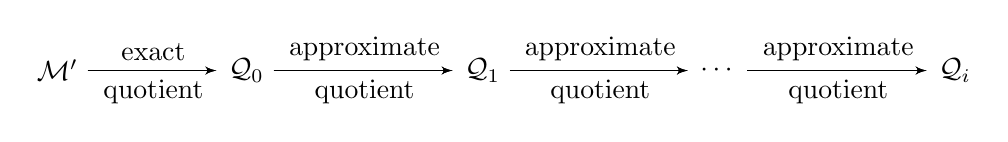
\begin{tikzpicture}[xscale=.6,>=latex',shorten >=1pt,node distance=3cm,on grid,auto]
	
	\node[label] (Me) at (0,0) {$\Hyp$};
	\node[label] (Q0) at (4,0) {$\Q_{0}$};
	\node[label] (Q1) at (9,0) {$\Q_{1}$};
	\node[label] (Qd) at (14,0) {$\cdots$};
	\node[label] (Qi) at (19,0) {$\Q_{i}$};
	
	\path[->] (Me) edge node [midway, above] {exact} (Q0);
	\path[->] (Me) edge node [midway, below] {quotient} (Q0);	
	\path[->] (Q0) edge node [midway, above] {approximate} (Q1);
	\path[->] (Q0) edge node [midway, below] {quotient} (Q1);	
	\path[->] (Q1) edge node [midway, above] {approximate} (Qd);	
	\path[->] (Q1) edge node [midway, below] {quotient} (Qd);				
	\path[->] (Qd) edge node [midway, above] {approximate} (Qi);		
	\path[->] (Qd) edge node [midway, below] {quotient} (Qi);		
	%\path[->] (Meq) edge node [midway, below] {minimisation} (MOut);				
	\end{tikzpicture}
	\caption{Overview of the minimisation algorithms. \cref{lemma:additivity-property} applies to $\Hyp$, $\Q_{0}$, $\Q_{1}, \cdots, \Q_{i}$.}\label{fig:algorithms}
\end{figure}

In this section, we present two practical minimisation algorithms that compute approximate quotients of $\Hyp$. Given an LMC $\Hyp = <S, L, \tauHyp, \ell>$ with perturbed transition probabilities and a small compression parameter $\epsilon_2$. Both algorithms start by computing $\Q_0$, the exact quotient of $\Hyp$.  They proceed in iterations and compute a sequence of approximate quotients where the approximate quotient ($\Q_{i}$) computed at the end of the $i$th iteration is an $\epsilon_2$-quotient of the quotient ($\Q_{i-1}$) given at the beginning of that iteration. Using the additivity lemma, we can show that the (approximate) quotient $\Q_i$ after the $i$th iteration is an $i\epsilon_2$-quotient of $\Hyp$. See \cref{fig:algorithms} for an overview of this approach. Each iteration computes a partition of the state space, lumps the states that are together in the partition and concludes with taking the exact quotient.

%In this section, we present two practical minimisation algorithms that compute approximate quotients of $\Hyp$. Both algorithms proceed in iterations and compute a sequence of approximate quotients. In each iteration, the algorithms first compute a partition of the state space of an approximate quotient and then lump the states that are together in the partition. The exact quotient of the LMC after lumping is used as the new approximate quotient. The first approximate quotient $\Q_0$ is obtained by (exact) quotienting $\Hyp$ and it is guaranteed that the new approximate quotient obtained after lumping is an $\epsilon_2$-approximate quotient of the LMC before lumping. Using the additivity lemma, we can show that the approximate quotient generated by either algorithm after the $i$'s iteration is an $i\epsilon_2$-quotient of $\Hyp$. See \cref{fig:algorithms} for an overview of the algorithms.

\subsection{Local Bisimilarity Distance}\label{subsection:local-bisimilarity-distances}

We define the notion of \emph{local bisimilarity distance}, denoted by $d_{\local}^{\M}$ (or $d_{\local}$ when $\M$ is clear). Intuitively, two states $s$ and $t$ are at small local bisimilarity distance if they are probabilistic bisimilar in an LMC which is slightly perturbed only at the successor distributions of $s$ and~$t$. We provide a polynomial-time algorithm to compute the local bisimilarity distance. Given an LMC $\Hyp = <S, L, \tauHyp, \ell>$ (with perturbed transition probabilities) and a small compression parameter $\epsilon_2$, we propose an iterative minimisation algorithm to compute approximate quotients of $\Hyp$ by merging state pairs with small local bisimilarity distances. In each iteration of the algorithm, we select the state pair with the same label and the minimum local bisimilarity distance if such distance is at most $\epsilon_2$. We compute a partition in which this state pair are together and lump together the states that are together in the partition. The algorithm terminates when no pairs can be lumped, that is, all state pairs have local bisimilarity distances greater than $\epsilon_2$. %The LMC after lumping a state pair is an $\epsilon_2$-approximate quotient of the LMC before merging. Using the additivity lemma, the approximate quotient obtained by this algorithm after the $i$'s iteration is an $i\epsilon_2$-quotient of $\Hyp$.

% We then merge the states for which this distance is small. For the remainder of the section, we fix an approximation LMC $\Hyp = <S, L, \tauHyp, \ell>$ and a small error parameter $\epsilon_2$. The minimisation algorithm runs in iterations. In each iteration, we compute the local bisimilarity distances for all pairs of states with the same label. We merge the pair of states $s$ and $t$ with the same label such that it has the minimum local bisimilarity distance at most $\epsilon_2$. The algorithm terminates when no pairs can be merged, that is, all pairs of states have local bisimilarity distance greater than $\epsilon_2$.

 \paragraph*{Computing Local Bisimilarity Distances}\label{subsubsection:computeLocalBisimilarityDistances}
Given two different states $s, t \in S$ with the same label. We want to compute a new transition function $\tauHyp'$ by only changing the successor distributions of $s$ and $t$ ($\tauHyp(s)$ and $\tauHyp(t)$, respectively) such that $\{s, t\}$ belongs to an $\R$-induced partition where $\R$ is a probabilistic bisimulation of the LMC $\Hyp' = <S, L, \tauHyp', \ell>$. Let ${\rm T}$ be the set of the all transition functions that satisfy this condition, more precisely, we define ${\rm T} = \{\tauHyp' \suchthat \tauHyp'(x) = \tauHyp(x) \; \forall x \not\in \{s, t\}  \land \{s, t\} \in S /_{\R} \text{ where } \R \text{ is a probabilistic bisimulation of the LMC } \Hyp' = <S, L, \tauHyp', \ell>\}$. The local bisimilarity distance is defined as $d_{\local}^{\Hyp}(s, t) = \textstyle\inf_{\tau' \in {\rm T}} \max\{\|\tau'(s) - \tauHyp(s)\|_1, \|\tau'(t) - \tauHyp(t)\|_1 \}$. It is not immediately clear how to compute it. %Since for all $\tau' \in {\rm T}$, we have $s \sim t$ in the LMC $<S, T, \tau', \ell>$, it is not hard to see that $d^{\Hyp}_{\glob}(s, t) \le d_{\local}^{\Hyp}(s, t)$, that is, $d_{\local}^{\Hyp}(s, t)$ is an upper bound of $d^{\Hyp}_{\glob}(s, t)$.

%[not working] the required partition can be obtained simply by the following three steps: (1) construct a new LMS M’ from M by making both s and t absorbing; (2) compute the equivalence classes Y of M’ according to probabilistic bisimilarity; (3) delete s and t from Y and put back a new equivalence class {s, t}.
By the definition of ${\rm T}$, the probabilistic bisimulation $\R$ is the same for any LMC $<S, L, \tauHyp', \ell>$ with $\tauHyp' \in {\rm T}$. Let us define the partition $X = S /_\R$ where $\R$ is the common probabilistic bisimulation. The local bisimilarity distance can be computed by using $X$:
%Let us fix a transition function $\tauHyp' \in {\rm T}$ and fix an LMC $\Hyp' = <S, L, \tauHyp', \ell>$. To compute the local bisimilarity distance, we first compute the partition $X$ containing $\{s, t\}$ which is induced by the probabilistic bisimulation $\R$ of the LMC $\Hyp'$. It is noted that by the definition of ${\rm T}$, the probabilistic bisimulation $\R$ is the same for any LMC $<S, L, \tau', \ell>$ with $\tau' \in {\rm T}$. We then show that the local bisimilarity distance is half of the $L_1$-distance between $(\tau_{\epsilon}(s)(E))_{E \in X}$ and $(\tau_{\epsilon}(t)(E))_{E \in X}$: %, that is, $d_{\local}^{\Hyp}(s, t) = \frac{1}{2} |(\tau_{\epsilon}(s)(E))_{E \in X} -(\tau_{\epsilon}(s)(E))_{E \in X}|$.

%The partition $X = S /_{\R}$ can simply be computed by the following two steps: (1) construct a new LMC from $\Hyp$ by introducing a new label, labelling both $s$ and $t$ with the new label and making both $s$ and $t$ absorbing; (2) compute the equivalence classes of this new LMC according to probabilistic bisimilarity. The resulting equivalence classes is $X$.  %by \cref{alg:s-t-partition-refinement}. Given a partition $Y$, we say $u \equiv_{Y} v$ in the LMC $<S, L, \tauHyp, \ell>$ if and only if $\ell(u) = \ell(v)$ and $\tauHyp(u)(E) = \tauHyp(v)(E)$ for all $E \in Y$.


%By definition of the set $\rm T$, the probabilistic bisimulation which contains $\{s, t\}$ of an LMC $\Hyp' = <S, L, \tauHyp', \ell>$ is the same for any $\tauHyp' \in {\rm T}$. This common probabilistic bisimulation induces a common partition over $S$, denoted by $X$, which is computed by \cref{alg:s-t-partition-refinement}.



%\begin{algorithm}[h]
%	\DontPrintSemicolon
%	
%	$i = 0; Y_0 := \big\{ \{s, t\}, S \setminus \{s, t\} \big\}$\;
%	\Repeat{$Y_i = Y_{i-1}$}{
%		$i := i+1$\;
%		$Y_{i} :=S/\mathord{\equiv_{Y_{i-1}}}$ \;
%		$Y_{i} := \big( (Y_{i} \setminus \{s\} ) \setminus \{t\} \big)  \cup \{\{s, t\}\}$\;
%	}
%	\caption{Partition refinement with $\{s, t\}$ in the final partition.}
%	\label{alg:s-t-partition-refinement}
%\end{algorithm}


\begin{restatable}{proposition}{propositionAdjustTransitionFunction}\label{proposition:adjust-transition-function-s-t}
%We have $d_{\local}^{\Hyp}(s, t) = \max\{|\tauHyp'(s) - \tauHyp(s)|, |\tauHyp'(t) - \tauHyp(t)| \} $ where $\tauHyp' \in {\rm T}$ is defined as \[
%\tauHyp'(x) = \left \{
%\begin{array}{ll}
%\tauHyp(x)& \mbox{if $x \not\in \{s, t\}$}\\
%\nu_x & \mbox{otherwise}
%\end{array}
%\right .
%\]
%Furthermore,
We have $d_{\local}^{\Hyp}(s, t) =	 \frac{1}{2} \|(\tau_{\epsilon}(s)(E))_{E \in X} -(\tau_{\epsilon}(t)(E))_{E \in X}\|_1$.
%We have $d_{\local}^{\Hyp}(s, t) = \max\{ |\tauHyp'(s) - \tauHyp(s)| , |\tauHyp'(t) - \tauHyp(t)|\}$ where
%$\tauHyp' \in {\rm T}$ is defined as $\tauHyp'(x) = \tauHyp(x)$ for all $x \not\in \{s, t\}$ and $\tauHyp'(x) = \nu_x$ if $x \in \{s, t\}$.
\end{restatable}

It turns out that $X$ can simply be computed by \cref{alg:local-distance-partition}. As this algorithm is basically taking the (exact) quotient of the LMC constructed on line~1, it runs in polynomial time. It follows from \cref{proposition:adjust-transition-function-s-t} that the local bisimilarity distance can be computed in polynomial time.

%The partition $X = S /_{\R}$ can simply be computed by the following two steps: (1) construct a new LMC from $\Hyp$ by introducing a new label, labelling both $s$ and $t$ with the new label and making both $s$ and $t$ absorbing; (2) compute the equivalence classes of this new LMC according to probabilistic bisimilarity. The resulting equivalence classes constitute $X$.  %by \cref{alg:s-t-partition-refinement}. Given a partition $Y$, we say $u \equiv_{Y} v$ in the LMC $<S, L, \tauHyp, \ell>$ if and only if $\ell(u) = \ell(v)$ and $\tauHyp(u)(E) = \tauHyp(v)(E)$ for all $E \in Y$.

\begin{algorithm}[h]
	\DontPrintSemicolon
	\KwIn{An LMC $\Hyp = <S, L, \tauHyp, \ell>$, a state pair $(s, t) \in S \times S$}
	\KwOut{A partition $X$ over $S$ containing $\{s, t\}$}
	Construct a new LMC $\Hyp'$ from $\Hyp$ by introducing a new label, labelling both $s$ and $t$ with the new label and making both $s$ and $t$ absorbing\footnotemark\;
	$X := S /_{\sim_{\Hyp'}}$\;
	\caption{Compute Partition for Local Bisimilarity Distances}
	\label{alg:local-distance-partition}
\end{algorithm}
\footnotetext{\modify{An absorbing state is a state that, once entered, cannot be left; that is, a state with self-loop.}}

\begin{example}\label{example:intro3}
 Assume $\epsilon \ls \frac{1}{2}$. Consider the LMC shown in \cref{fig:intro3}. Let $\tauHyp$ denote its transition function. To compute the local bisimilarity distance of $s_1$ and $t_1$, we first compute the partition containing $\{s_1, t_1\}$: $X = \big\{ \{ s_1, t_1\}, \{ s_2\},\{ t_2\} \big\}$. We have $(\tauHyp(s_1)(E))_{E \in X} = (\frac{1}{2}, \frac{1}{2}, 0)$ and $(\tauHyp(t_1)(E))_{E \in X} = (\frac{1}{2}+\epsilon, 0, \frac{1}{2}-\epsilon)$. By \cref{proposition:adjust-transition-function-s-t}, the local bisimilarity distance is $d_{\local}(s_1, t_1) = \frac{1}{2}\|(\tauHyp(s_1)(E))_{E \in X} -(\tauHyp(t_1)(E))_{E \in X}\|_1 = \frac{1}{2}$. Similarly, we have~$d_{\local}(s_2, t_2) =~\frac{1}{2}$.%~\qed
\end{example}

\begin{algorithm}[h]
	\DontPrintSemicolon
	\KwIn{An LMC $\Hyp = <S, L, \tauHyp, \ell>$, a compression parameter $\epsilon_2$}
	\KwOut{An LMC $\Q_{i}$}
	$i := 0$\\
	%$\M^{i}: = <S, L, \tau', \ell>$ \\	
	%Compute $\sim_{\Hyp}$\\
	$\Q_{i} := \Hyp/_{\sim_{\Hyp}}$ and $\Q_{i} = <S^{\Q_{i}}, L, \tau^{\Q_{i}}, \ell^{\Q_{i}}>$\;
	%$\Q_{i} = <S^{\Q_{i}}, L, \tau^{\Q_{i}}, \ell^{\Q_{i}}> := \M^{i}/_{\sim_{\M^{i}}}$ where $\M^{i} = \Hyp$\\	
	%$\Hyp^{i} = <S^{\Hyp^{i}}, L, \tau^{\Hyp^{i}}, \ell^{\Hyp^{i}}> := \M^{i}/_{\sim_{\M^{i}}}$ where $\M^{i} = \Hyp$\\
	\While{$\exists u, v \in S^{\Q_{i}} \text{ such that }  u \not= v \text{ and }  \ell^{\Q_{i}}(u) = \ell^{\Q_{i}}(v) \text{ and }  d_{\local}^{\Q_{i}} (u, v) \le \epsilon_2$ }{
		$(s, t) = \arg\min \{d_{\local}^{\Q_{i}} (u, v) \suchthat (u ,v) \in S^{\Q_{i}} \times S^{\Q_{i}} \land u \not= v \land   \ell^{\Q_{i}}(u) = \ell^{\Q_{i}}(v)\}$\\
		%Select two states $s, t \in S^{\Hyp^{i}}$ where $\ell^{\Hyp^{i}}(s) = \ell^{\Hyp^{i}}(t)$ and $d_{\local}^{\Hyp^{i}} (s, t) = \min\limits_{u ,v \in S^{\Hyp^{i}} \text{ and } \ell^{\Hyp^{i}}(u) = \ell^{\Hyp^{i}}(v)} d_{\local}^{\Hyp^{i}} (u, v)$\\
		%Compute $\sim_{\Hyp^{i}}$\\
		%		Compute $X$ by Algorithm~\ref{alg:s-t-partition-refinement} with the input LMC $\Hyp^{i}$ and $\{s, t\}$\;
		%		$\gamma := \frac{(\tau^{\Hyp^{i}}(s))_{E \in X} + (\tau^{\Hyp^{i}}(t))_{E \in X}}{2}$ \;
		%		$\nu_s$ (resp. $\nu_t$) is obtained by running \cref{alg:adjust-transition-probability} with $X$, $\tau^{\Hyp^{i}}(s)$ (resp. $\tau^{\Hyp^{i}}(t)$) and $\gamma$\;
		%		$
		%		\tau'(x) := \left \{
		%		\begin{array}{ll}
		%		\tau^{\Hyp^{i}}(x)& \mbox{if $x \not\in \{s, t\}$}\\
		%		\nu_x & \mbox{otherwise}
		%		\end{array}
		%		\right .
		%		$\;
		%		$\M^{i+1} := <S^{\Hyp^{i}}, L, \tau', \ell^{\Hyp^{i}}>$ \;
		%Construct an LMC $\Q_{i}'$ from $\Q_{i}$ by adding a new label, labelling $s$ and $t$ with this new label and making $s$ and $t$ absorbing \; %$\M_{i+1}$
		%Compute $\M_{i+1}: = \Q_{i}'/_{\sim_{\Q_{i}'}}$ with state space $X_i := S^{\Q_{i}'} /_{\sim_{\Q_{i}'}}$\;
		Compute $X_i$ by running \cref{alg:local-distance-partition} with input $Q_i$ and $(s, t)$\;
		Construct an LMC $\M_{i+1}:= <X_i, L, \tau^{\M_{i+1}}, \ell^{\M_{i+1}}>$ from $\Q_{i}$ where
		$
		\tau^{\M_{i+1}}(E) := \left \{
		\begin{array}{l}
		 (\tau^{\Q_{i}}(u)(E'))_{E' \in X_i}  \mbox{ for any $u \in E$ if $E \in X_i$  and $E \not= \{s, t\}$}\\
		\frac{(\tau^{\Q_{i}}(s)(E'))_{E' \in X_i} + (\tau^{\Q_{i}}(t)(E'))_{E' \in X_i}}{2} \;\; \mbox{if $E = \{s, t\}$}\\
		\end{array}
		\right .
		$ and $\ell^{\M_{i+1}} (E) := \ell^{\Q_i}(u)$ for $E \in X_i$ and any $u \in E$\;
		
		%from $\Q_{i}$ by restoring the labels of $\{s, t\}$ and setting the probability distribution from $\{s, t\}$ as $\frac{(\tau^{\Q_{i}}(s))_{E \in X_i} + (\tau^{\Q_{i}}(t))_{E \in X_i}}{2}$\;
		%Obtain the new approximate quotient LMC $\Q_{i+1}$ by quotienting $\M_{i+1}'$, that is,
		$\Q_{i+1} := \M_{i+1} /_{\sim_{\M_{i+1}}}$\;
		$i := i+1$\;
	}
	\caption{LMC Minimisation Using Local Bisimilarity Distances}
	\label{alg:local-distance-merge-algorithm}
\end{algorithm}

\paragraph*{Minimisation Algorithm Using Local Bisimilarity Distances}
\label{subsubsection:minimisation-algorithm-local-bisimilarity-distances}
\cref{alg:local-distance-merge-algorithm} shows the minimisation algorithm using local bisimilarity distances. The input is an LMC $\Hyp$ and a compression parameter $\epsilon_2$. We start by initializing an index $i$ to $0$ and building the quotient LMC $\Q_{0} = \Hyp /_{\sim_{\Hyp}}$. If there are no states in $\Q_{i}$ with local bisimilarity distance less than $\epsilon_2$, the algorithm terminates. Otherwise, it steps into the $i$'th iteration of the loop and computes the local bisimilarity distances for all pairs of states in $\Q_{i}$ with the same label. It selects the state pair $(s, t)$ which has the smallest local bisimilarity distance on line~4. It then computes the new approximate quotient by merging states $s$ and $t$ on line~$5$-$7$. This computation is in three steps where the first step is to compute the partition $X_i$ (line~5) by running \cref{alg:local-distance-partition} with input $\Q_i$ and the state pair $(s, t)$. The second step is to construct a new LMC $\M_{i+1}$ by setting $X_i$ as its state space (line~6). The final step is to compute a new approximate quotient $\Q_{i+1}$ by taking the exact quotient of the LMC $\M_{i+1}$ obtained from the previous step.
%A new transition function $\tau'$ (line~5-8) as described by \cref{proposition:adjust-transition-function-s-t} and a new LMC $\M^{i+1}$ with $\tau'$ as its transition function is constructed on line~9. We then compute its quotient $\Hyp^{i+1} = \M^{i+1} /_{\sim_{\M^{i+1}}}$. The size of the state space of $\Hyp^{i+1}$ will decrease by at least one as $s \sim_{\M^{i+1}} t$.
We increment $i$ at the end of the iteration and continue with another iteration if there are states in $\Q_{i+1}$ with local bisimilarity distance at most $\epsilon_2$. Since there are finitely many states and it is polynomial time to compute the local bisimilarity distances, the algorithm always terminates and runs in polynomial time.
%The first minimisation algorithm is shown in Algorithm~\ref{alg:local-distance-merge-algorithm} . The input is a hypothesis LMC $\Hyp$ and an error parameter $\epsilon_2$. We start by building the quotient LMC $\Hyp^{i} = \Hyp /_{\sim_{\Hyp}}$ with $i$ initialized to $0$. It then steps into a loop with incrementing $i$ at the beginning. In the $i$'th iteration of the loop, it computes the local bisimilarity distances for all pairs of states in $\Hyp^{i-1}$ with the same label and selects the pair $s$ and $t$ which have the least local bisimilarity distance. We obtain a new LMC $\M^{i}$ by adjusting the transition probability distribution at $s$ and $t$. It is done by replacing the transition function $\tau^{\Hyp^{i-1}}$ of $\Hyp^{i-1}$ with $\tau'' = \adjust(\tau^{\Hyp^{i-1}}, s, t, u)$ where $\tau''$ yields the local bisimilarity distance of $s$ and $t$, that is, $d_{\local}^{\Hyp^{i-1}} (s, t) = \max\{|\tau^{\Hyp^{i-1}}(s) - \tau''(s) |, |\tau^{\Hyp^{i-1}}(t) - \tau''(t)|\}$. We then build the new quotient LMC $\Hyp^{i} = \M^{i} /_{\sim_{\M^{i}}}$. If the size of the state space of $\Hyp^{i}$ decreases we continue the iteration. Otherwise, the algorithm terminates since there are no states in $\Hyp^{i}$ with local bisimilarity distance less than $\epsilon_2$. Since there are finitely many states, the algorithm always terminates.

%%$\Pr(d_{\glob}^{\M \oplus \Hyp^{i}} (x, x') \le \epsilon + i \epsilon_2) \ge (1-\delta)^{|S|}$
%\begin{restatable}{theorem}{theoremBoundingGlobalDistance}\label{theorem:bounding-global-distance} Let $d_{\glob}^{\M \oplus \Hyp} (x, x') \le \epsilon$ for all state $x$ in $\M$ and the corresponding state $x'$ in $\Hyp$. For all $i \in \nat$, we have $d_{\glob}^{\M \oplus \Hyp^{i}} (x, x') \le \epsilon + i \epsilon_2$ where $x$ is a state in $\M$ and $x'$ is the corresponding state in $\Hyp^{i}$.
%\end{restatable}
%
%
%\begin{corollary}\label{corollary:bounding-global-distance-local-distance}
%	For all $i \in \nat$, we have $\Pr(d_{\glob}^{\M \oplus \Hyp^{i}} (x, x') \le \epsilon + i \epsilon_2) \ge (1-\delta)^{|S|}$ where $x$ is a state in $\M$ and $x'$ is the corresponding state in $\Hyp^{i}$.
%\end{corollary}
%\begin{proof}
%Let $i \in \nat$. Let $x$ be a state from $\M$ and $x'$ be the corresponding state from $\Hyp^{i}$. Let $x_h$ of $\Hyp$ correspond to $x$ of $\M$. By $\Pr(d_{\glob}^{\M \oplus \Hyp} (x, x_h) \le \epsilon ) \ge (1-\delta)^{|S|}$ and \cref{theorem:bounding-global-distance}, we have $\Pr(d_{\glob}^{\M \oplus \Hyp^{i}} (x, x') \le \epsilon + i \epsilon_2) \ge (1-\delta)^{|S|}$.
%\end{proof}

%Merging by approximate partition refinement
\subsection{Minimisation by Approximate Partition Refinement}\label{subsection:approximate-partition-refinement}
%an example LMC that could not be merged by the previous algorithm
Consider the LMC in \cref{fig:intro3}. Assume $\epsilon \ls \frac{1}{2}$ and $\epsilon_2 \ls \frac{1}{2}$. The minimisation algorithm using local bisimilarity distance (Algorithm~\ref{alg:local-distance-merge-algorithm}) cannot merge states $s_1, t_1$ (or $s_2, t_2$) as $d_{\local}(s_1, t_1) = d_{\local}(s_2, t_2)  =\frac{1}{2} \gr \epsilon_2$ as shown by \cref{example:intro3}.

We introduce an approximate partition refinement, a polynomial algorithm similar to the exact partition refinement, which can fix this problem. In the exact partition refinement algorithm, the states will only remain in the same set in an iteration if they have the same label and their probability distributions over the previous partition are the same. Similarly, we design the approximate partition refinement such that states only remain in the same set in an iteration if they have the same label and the $L_1$-distance between the probability distributions over the previous partition is small, say, at most $\epsilon_2$. Given an LMC $\Hyp = <S, L, \tauHyp, \ell>$ with perturbed transition probabilities, the minimisation algorithm using the approximate partition refinement also proceeds in iterations. In each iteration, the approximate partition refinement computes a partition $X$ and then the states which are together in $X$ are  lumped to form a new LMC. To make sure the new LMC is a quotient, we take the (exact) quotient of this LMC as our new approximate quotient. The algorithm continues when there are states that could be lumped, and it terminates when all sets in the partition computed by the approximate partition refinement are singletons, that is, no states can be lumped. %We prove that the LMC after merging is an $\epsilon_2$-approximate quotient of the LMC before merging. Similar to the previous minimisation algorithm, using the additivity lemma, the approximate quotient obtained by this algorithm after the $i$'s iteration is an $i\epsilon_2$-quotient of $\Hyp$.%Using the additivity lemma, we can then bound the error of the final approximate quotient obtained by this algorithm.% guarantees that states in an equivalence class of the final partition have small global bisimilarity distances and thus can be merged.

\modify{
	\begin{example}\label{example:approximate-partition-intro}	
	Consider again the LMC in \cref{fig:intro3}. Assume $\epsilon \ls \frac{1}{2}$ and the compression parameter $\epsilon_2 \ge 2\epsilon$.  We run the above-mentioned minimisation algorithm using the approximate partition refinement. It will only run for one iteration of approximate partition refinement, as we will see in the following. \Cref{fig:example-intro-approximate-partition-refinement}(a) shows the partitions of this iteration. At the beginning of the approximate partition refinement, we have partition $X_0$ as all states are in the same set. The states are then split by the labels and we get partition $X_1$. There is no further split since the $L_1$-distance between the probability distributions over $X_1$ from $s_1$ and $t_1$ (resp. $s_2$ and $t_2$) is $2\epsilon$ which is bounded by the compression parameter $\epsilon_2$, that is, $\|(\tau(s_1)(E))_{E \in X_1}  - (\tau(t_1)(E))_{E \in X_1}\|_1 = \|(\tau(s_2)(E))_{E \in X_1}  - (\tau(t_2)(E))_{E \in X_1}\|_1 = 2\epsilon \le \epsilon_2$. The states together in $X_1$ are then lumped to form the new LMC shown in \cref{fig:example-intro-approximate-partition-refinement}(b). The algorithm terminates as no states in the new LMC can be lumped.
	\end{example}
}

\begin{figure}
\begin{minipage}{0.45\textwidth}
	\centering	\vspace{0.2cm}
	\begin{tabular}{l}
		\\\\\\
		\hline%wd{0.5pt}
		$X_0 = \{S\}$ \\
		$X_1 = \big\{  \{s_1,t_1\} , \{s_2,t_2\} \big\}$\\
		\hline
		\\\\
		(a) The partitions.
	\end{tabular}
	%\captionof{table}{The partitions.} \label{tab:example-intro-approximate-partition-refinement}
\end{minipage}
\hfill
\begin{minipage}{0.45\textwidth}
	\centering
\tikzstyle{BoxStyle} = [draw, circle, fill=black, scale=0.4,minimum width = 1pt, minimum height = 1pt]

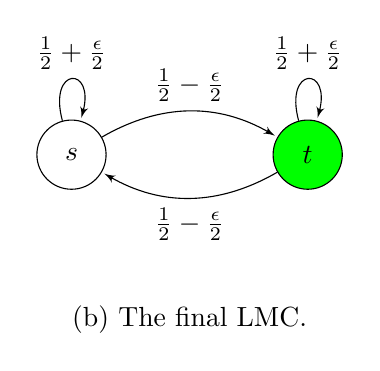
\begin{tikzpicture}[scale=.6,>=latex',shorten >=1pt,node distance=3cm,on grid,auto]

%\node[label]  at (2,2.7) {the MC~$\C$};

\node[state] (s) at (-1,0) {$s$};
\node[state, fill=green] (s2) at (4,0) {$t$};


%	\node[state] (u) at (19,0) {$u_1$};
%	\node[state, fill=green] (u2) at (24,0) {$u_2$};

\path[->] (s) edge [out=30,in=150] node [midway, above] {$\frac{1}{2}-\frac{\epsilon}{2}$} (s2);
\path[->] (s2) edge [out=210,in=-30] node [midway, below] {$\frac{1}{2}-\frac{\epsilon}{2}$} (s);

	\path[->] (s) edge [loop above]node [midway, above] {$\frac{1}{2} +\frac{\epsilon}{2}$} (s);
\path[->] (s2) edge [loop above] node [midway, above] {$\frac{1}{2} +\frac{\epsilon}{2} $} (s2);

\node at (1.5,-3.5) {(b) The final LMC.};
\end{tikzpicture}
%	\captionof{figure}{The final LMC.} \label{fig:example-intro-approximate-partition-refinement}
\end{minipage}
\caption{Example of running the minimisation algorithm using approximate partition refinement (Algorithm~\ref{alg:polynomial-optimistic-partition-refinement}) on the LMC in \cref{fig:intro3}.} \label{fig:example-intro-approximate-partition-refinement}
\end{figure}

%the approximate partition refinement
\paragraph*{Approximate Partition Refinement}
\begin{algorithm}[h]
	%		\setstretch{1.12}
	\DontPrintSemicolon
	\KwIn{An LMC $\Hyp = <S, L, \tauHyp, \ell>$, a compression parameter $\errorParam$}
	\KwOut{A partition $X$ over $S$}	
	$i := 0; X_0 := \{S\}$\;
	\Repeat{$X_i = X_{i-1}$}{
		$i := i+1$; $X_i := \emptyset$\;
		\ForEach{$E \in X_{i-1}$}{
			$X_E := \emptyset$\;
			%add $E': = \{s\}$ to $X_E$ where $s \in E$ \;		
			\For{$s \in E$}{
				$ESet := \{E'\in X_{E} \suchthat \text{for all } t\in E' \text{ we have } \ell(s)=\ell(t) \text{ and}\linebreak \|(\tauHyp(s)(E))_{E \in X_{i-1}} - (\tauHyp(t)(E))_{E \in X_{i-1}}\|_1 \le \epsilon_2 \}$\;
				\lIf{$ESet = \emptyset$}{
					$E': = \{s\}$
				}\Else{
					$E' := \arg\min\limits_{E' \in ESet}\big\{ \frac{\sum_{t \in  E'} \|(\tauHyp(s)(E))_{E \in X_{i-1}} - (\tauHyp(t)(E))_{E \in X_{i-1}}\|_1}{|E'|} \big\}$\;
					remove $E'$ from $X_E$; $E' := E' \cup \{ s \}$\;
				}
				add $E'$ to $X_E$ \;
			}
			$X_i := X_i \cup X_E$\;
		}
	}
	\caption{\mbox{Approximate Partition Refinement}}
	\label{alg:polynomial-optimistic-partition-refinement}
\end{algorithm}

Given a compression parameter $\epsilon_{2}$, the approximate partition refinement is shown in Algorithm~\ref{alg:polynomial-optimistic-partition-refinement}. At the beginning, an index $i$ is initialized to zero and we have $X_0 = \{S\}$, that is, all states are in the same set. In a refinement step, we increment $i$ and split each set $E \in X_{i-1}$ into one or more sets. We iterate though all $E \in X_{i-1}$ and for each $E$ we construct a set $X_E$, a partition of $E$. Starting with $X_E = \emptyset$, we iterate over all $s \in E$ (line~6). After each iteration, the current $s \in E$ appears in one set in $X_E$: either as a singleton or as an additional state in an already existing set in $X_E$. We give more details on this loop (lines~6-14) below.
After having partitioned~$E$ into~$X_E$, we add all sets in~$X_E$ to the new partition~$X_i$.
The way we split the sets ensures that for any two states from the same set in~$X_i$ the $L_1$-distance between the successor distributions over $X_{i-1}$ is at most $\epsilon_2$. The algorithm terminates when no splitting can be done.
Let $X$ be the final partition produced by the approximate partition refinement. For any two states $s, t \in E$ where $E \in X$, we have $\ell(s) = \ell(t)$ and $\|(\tauHyp(s)(E'))_{E' \in X} - (\tauHyp(t)(E'))_{E' \in X}\|_1 \le \epsilon_2$.

Let us give more details on the loop (lines~6-14) that partitions an $E \in X_i$.
For a state $s \in E$, a candidate set $\mathit{ESet}$ is computed such that for all $E' \in \mathit{ESet}$ the state $s$ and all $x \in E'$ have the same label and the $L_1$-distance between the successor distributions over $X_{i-1}$ of $s$ and any $x \in E'$ is at most $\epsilon_2$ (line~7). If $\mathit{ESet}$ is empty, we add the singleton $\{s\}$ into $X_E$ (line~8 and~13). If there is only one set $E'$ in $\mathit{ESet}$, we add $s$ to the set $E'$. Otherwise, if there are multiple elements in $\mathit{ESet}$ that satisfy the condition, we select the one as $E'$ such that the average $L_1$-distance between the successor distributions of $s$ and $x \in E'$ is the smallest (line~10). We add $s$ to the selected set $E'$ and include $E'$ in $X_{E}$ (line~10-13).


%which is also a set of $X_E$ by adding $s$

%If such $\mathit{ESet}$ is not empty, we select a set $E'$ from $\mathit{ESet}$ such that the average $L_1$-distance between $s$ and $x \in E'$ is the smallest (line~12). We then update $E'$ which is also a set of $X_E$ by adding $s$ (line~13-16).

\paragraph*{Minimisation Algorithm Using Approximate Partition Refinement}


\begin{algorithm}[h]
	\DontPrintSemicolon
	\KwIn{An LMC $\Hyp = <S, L, \tauHyp, \ell>$, a compression parameter $\epsilon_2$}
	\KwOut{An LMC $\Q_{i}$}
	$i := 0$\\
	%$\M^{i}: = <S, L, \tau', \ell>$ \\	
	%Compute $\sim_{\Hyp}$\\
	$\Q_{i} := \M_{i}/_{\sim_{\M_{i}}}$ where $\M_{i} = \Hyp$ and $\Q_{i} = <S^{\Q_{i}}, L, \tau^{\Q_{i}}, \ell^{\Q_{i}}>$ \;
	%$\omega' = \omega$\\
	%$d_{u, v} = 0 \forall u, v$ \\
	\Repeat{$|S^{\Q_{i}}| = |S^{\Q_{i-1}}|$}{
		Compute $X_i$ by running Algorithm~\ref{alg:polynomial-optimistic-partition-refinement} with $\Q_{i} $ and $\epsilon_2$ as input\;
		Construct an LMC $\M_{i+1} :=  <X_i, L , \tau^{\M_{i+1}}, \ell^{\M_{i+1}} >$ from $\Q_i$ where $\tau^{\M_{i+1}}(E) := \sum_{u \in  E}  \frac{(\tau^{\Q_{i}}(u)(E'))_{E' \in X_i}}{|E|}$ and $\ell^{\M_{i+1}}(E) := \ell^{\Q_{i}}(x)$ for all $E \in X_i$ and any $x \in E$\;
		% such that $\M_{i+1} :=  <X_i, L , \tau^{\M_{i+1}}, \ell^{\M_{i+1}} >$
		%		\ForEach{$x \in S^{\Hyp^{i-1}}$}{
		%			$\gamma_x := \sum_{u \in  E_x} \frac{(\tau^{\Hyp^{i-1}}(u)(E))_{E \in X}}{|E_x|}$ where $x \in E_x$ and $E_x \in X$\;
		%			$\nu_x$ is obtained by running \cref{alg:adjust-transition-probability} with $X$, $\tau^{\Hyp^{i-1}}(x)$ and $\gamma_x$\;
		%			$\tau'(x) = \nu_x$ \;
		%		}
		%		$\M^{i}: = <S^{\Hyp^{i-1}}, L, \tau', \ell^{\Hyp^{i-1}}>$\;
		%		$\Hyp^{i} :=\M^{i} / \sim_{\M^{i}}$ and $\Hyp^{i} = <S^{\Hyp^{i}}, L, \tau^{\Hyp^{i}}, \ell^{\Hyp^{i}}>$ \;
		%Obtain the new approximate quotient $\Q_{i+1}$ by exact quotienting $\M_{i+1}$, that is,
		$\Q_{i+1} := \M_{i+1} /_{\sim_{\M_{i+1}}}$\;
		$i := i+1$ \;
	}
	\caption{LMC Minimisation by Approximate Partition Refinement}
	\label{alg:approximate-partition-refinement-merge-algorithm}
\end{algorithm}

The minimisation algorithm using approximate partition refinement is shown in \cref{alg:approximate-partition-refinement-merge-algorithm}. The input is the same as the first minimisation algorithm: an LMC $\Hyp$ and a compression parameter $\epsilon_2$. An index $i$ is initialised to $0$. Similar to the approximate minimisation algorithm using local bisimilarity distances, we also start by computing the quotient LMC $\Q_{0} = \Hyp/_{\sim_{\Hyp}}$. It then steps into a loop. We compute the approximate partition $X_i$ of $\Q_{i}$ on line~4 and construct a new LMC $\M_{i+1}$ by setting $X_i$ as its state space on line~5. For any state $E \in X_i$, we set the probability distribution as the average probability distribution over $X_i$ from all $u \in E$. The label of any $E \in X$ is set to $\ell^{\Q_{i}}(u)$ where $u$ can be any state from $E$. A new approximate quotient $\Q_{i+1} $ is obtained by taking the exact quotient of $\M_{i+1}$. We increment $i$ at the end of the iteration and continue another iteration if the size of the state space of the new approximate quotient decreases. Otherwise, the algorithm terminates as we have no states to merge. As there are finitely many states, the algorithm always terminates.

%On line~5-10, we construct a new transition function $\tau'$ as described by \cref{proposition:transition-function-small-difference} and obtain a new LMC $\M^{i}$ by using $\tau'$ as its transition function.


Let $i \in \nat$. The following theorem applies to both the LMCs $\Q_{i}$ from \cref{alg:local-distance-merge-algorithm} and those from \cref{alg:approximate-partition-refinement-merge-algorithm}.
\begin{restatable}{theorem}{theoremBoundGlobalDistanceApproximatePartitionRefinement}\label{theorem:bounding-global-distance}
 %Let $d_{\glob}^{\M \oplus \Hyp} (x, x') \le \epsilon$ for all state $x$ in $\M$ and the corresponding state $x'$ in $\Hyp$.
 For all $i \in \nat$, we have that $\Q_{i+1}$ is an $\epsilon_2$-quotient of $\Q_i$. Furthermore, by the additivity lemma, we have that $\Q_i$ is an $i\epsilon_2$-quotient of $\Hyp$. %$d_{\glob}^{\Hyp^{0} \oplus \Hyp^{i}} (x, x_i) \le i \epsilon_2$ where $x$ is a state from $\Hyp^{0}$ and $x_i$ is the corresponding state in $\Hyp^{i}$.
\end{restatable}

In the case that $\Hyp=<S, L, \tauHyp, \ell>$ is a slightly perturbed version of $\M = <S, L,\tau,\ell>$, that is, for all $s \in S$ we have $\|\tau(s) - \tauHyp(s)\|_1 \le \epsilon$, the following corollary holds:
\begin{restatable}{corollary}{corollaryBoundQuotientError}\label{corollary:bounding-quotient-error}
 For all $i \in \nat$, we have that $\Q_i$ is an $(\epsilon + i\epsilon_2)$-quotient of $\M$.
\end{restatable}

 %with possibly imprecise transition probabilities.
%Let $\epsilon \gr 0$ be an error parameter. By slightly perturbed we mean that for each state the successor distributions in $\M_\epsilon$ and~$\M$ have small $L_1$-distance, i.e., at most $\epsilon$.	
%Since we have $R_{\epsilon} \subseteq \mathord{\sim_{\epsilon}}$ by \cref{proposition:approximate-global-relation-subset}, it follows from \cref{theorem:bounding-global-distance} that for all $i \in \nat$, $x \mathord{\sim_{i \epsilon_2}} x_i$ where $x$ is a state from $\Hyp^{0}$ and $x_i$ is the corresponding state in $\Hyp^{i}$.



\section{Active LMC Learning}
\label{section:active-LMC-learning}
%SETUP
%\begin{figure}[h]
%	\centering
%	
%	\begin{tikzpicture}[xscale=.6,>=latex',shorten >=1pt,node distance=3cm,on grid,auto]
%	
%	\node[label] (M) at (0,0) {$\M$};
%	\node[label] (Me) at (6,0) {$\Hyp$};
%	\node[label] (Meq) at (12,0) {$\Q_{0}$};
%	\node[label] (MOut) at (18,0) {$\Q_{i}$};
%	
%	\path[->] (M) edge node [midway, above] {perturbation} (Me);
%	\path[->] (M) edge node [midway, below] {(e.g., sampling)} (Me);
%	\path[->] (Me) edge node [midway, above] {exact quotient} (Meq);		
%	\path[->] (Meq) edge node [midway, above] {approximate} (MOut);		
%	\path[->] (Meq) edge node [midway, below] {minimisation} (MOut);				
%	\end{tikzpicture}
%	\caption{Workflow. \cref{lemma:additivity-property} is applied to $\M$, $\Q_{0}$ and $\Q_{i}$.}\label{fig:workflow}
%\end{figure}

%\subsection{Overall Approach}\label{subsection:learning-overall-approach}
%TODO In the first one (say "4A" for now), we describe our overall approach. I think we should say that we have an imprecise version of a (usually unknown) system. These two systems have small distance. For example, with sampling we can get this distance small with a high probability. (Notice that "high probability" only makes sense in the sampling context, not in general.) We also put the description of sampling in Section 4A.

%Let us assume that we do not have access to the transition probabilities of an LMC~$\M$. Rather, we have a slightly perturbed version $\Hyp=<S, L, \tauHyp, \ell>$ of $\M$. %with possibly imprecise transition probabilities.
%Let $\epsilon \gr 0$ be an error parameter. By slightly perturbed we mean that for each state the successor distributions in $\M_\epsilon$ and~$\M$ have small $L_1$-distance, i.e., at most $\epsilon$. For example, with sampling we can obtain with high probability a perturbed system that has small distance with $\M$.
%
%%TODO Then, still in 4A, we say that in the next section, say "4B" for now, we will present approximate minimisation algorithms. They produce a minimised system (i.e., a 3rd system) which has small distance from the perturbed system. We might give forward references to the theorems in 4B that claim this small distance.
%
%To compute an approximate quotient system of $\Hyp$, our first idea is to compute and merge states with small global bisimilarity distances. As it is $\sf NP$-complete to compute the global bisimilarity distances by \cref{theorem: global-epsilon-bisimulation-NP-complete}, this approach is not straightforward. Instead, in \cref{section:minimisation-algorithms}, we present two polynomial-time approximate minimisation algorithms. These two algorithms start by computing an LMC $\Hyp^{0}$, the exact quotient of $\Hyp$. With a compression parameter $\epsilon_2$ as input, they produce a minimised system $\Hyp^{i}$ where $i$ is the number of loop iterations of the two minimisation algorithms, respectively. From \cref{theorem:bounding-global-distance}, $\Hyp^{i}$ has global bisimilarity distance at most $i\epsilon_2$ from $\Hyp^{0}$, the exact quotient of the perturbed system.
%
%Together with the fact that $\M$ and $\Hyp$ (or its exact quotient $\Hyp^{0}$) have global bisimilarity distance at most $\epsilon$, it follows from \cref{lemma:additivity-property} that the minimised system $\Hyp^{i}$ and $\M$ have small global bisimilarity distance $\epsilon + i\epsilon_2$. \cref{fig:workflow} shows the workflow of our approach.

%TODO Then, still in 4A, we say that putting these two things together, by the triangle inequality (does it hold?), it follows that the unknown system has small distance to the minimised one. This holds with high probability if the imprecise chain has been obtained by sampling, and I think we can state that as a corollary (of the sampling theorem and the forward references).


%Let $\epsilon \gr 0$ be an error parameter and $\delta \gr 0$ be an error bound. Given a labelled Markov chain~$\M$ with possibly imprecise transition probabilities and a slightly perturbed version $\Hyp=<S, L, \tauHyp, \ell>$ of $\M$,  we hope to compute a compressed version of $\M$. By slightly perturbed we mean that for each state the successor distributions in $\Hyp$ and~$\M$ have $L_1$-distance which is at most~$\epsilon$ with probability at least $1 - \delta$. Next, we present how to obtain such approximation LMC by sampling.

%Our first idea is to merge states which have small global bisimilarity distances. However, as we have shown in \cref{theorem: global-epsilon-bisimulation-NP-complete} that it is $\sf NP$-complete to decide the global $\epsilon$-bisimulation, directly computing the global bisimilarity distances is highly inefficient. Alternatively, in \cref{subsection:local-bisimilarity-distances}, we provide a polynomial-time algorithm to compute an upper bound of the global bisimilarity distance. We can then merge the states for which this upper bound is small. In \cref{subsection:approximate-partition-refinement}, we introduce an approximate partition refinement, a polynomial algorithm similar to the exact partition refinement, which guarantees that states in an equivalence class of the final partition have small global bisimilarity distances and thus can be merged.

%\paragraph*{Approximation LMC by Sampling} \label{subsubsection:sampling}
We apply our approximate minimisation algorithms in a setting of active learning. Before that, we first describe how to obtain a perturbed LMC $\Hyp$ by sampling. Assume that we want to learn the transition probabilities of an LMC $\M$, that is, the state space, the labelling and the transitions are known. We also assume the system under learning (SUL) $\M$ could answer the query $\nxt$ which takes a state $s$ as input and returns a successor state of $s$ according to the transition probability distribution $\tau(s)$.

%Sampling
%We can approximate the transition probabilities via sampling.
Given a state $s$ of the LMC. We denote by $x_s$ the number of successor states of $s$ and by~$n_s$ the number of times we query the SUL on $\nxt(s)$. Let $N_{s,t}$ be the frequency counts of the query result $t$, that is, the number of times a successor state $t$ appears as the result returned by the queries. We approximate the transition probability distribution by $\tauHyp(s)$ where $\tauHyp(s)(t) = \frac{N_{s, t}}{n_s}$ for all successor states $t$ of $s$. (Such an estimator is called an empirical estimator in the literature.)

Intuitively, the more queries we ask the SUL, the more accurate the approximate probability distribution $\tauHyp(s)$ would be. In fact, the following theorem holds~\cite[Section~6.4]{BazilleGenestJegourelSun2020},~\cite{Chen2015}.

\begin{theorem}\label{theorem:sampling-size} Let $\epsilon \gr 0$ be an error parameter and $\delta \gr 0$ be an error bound. Let $s \in S$. We have $\Pr(\|\tau(s) - \tauHyp(s)\|_1 \le \epsilon) \ge 1 -\delta$ for $n_s \ge \frac{1}{2 \epsilon^{2}}\ln(\frac{2x_s}{\delta})$.
\end{theorem}

%Equivalently, for any $s \in S$, we have $\Pr(|\tau(s) - \tauHyp(s)| \le \epsilon) \ge (1-\delta)$ for $n_s \ge \frac{1}{2 \epsilon^{2}}\ln(\frac{2x_s}{\delta})$.
For each state $s \in S$, we query the SUL on $\nxt(s)$ for $n_s \ge \frac{1}{2 \epsilon^{2}}\ln(\frac{2x_s}{\delta})$ times. We can make $\delta$ small since it appears in the logarithmic term. We then approximate the transition function by $\tauHyp$ and construct a hypothesis LMC $\Hyp = <S, L, \tauHyp, \ell>$. Since the queries $\nxt(s)$ and $\nxt(t)$ for all $s,t \in S$ and $s \not= t$ are mutually independent, by Theorem~\ref{theorem:sampling-size}, we have that $\Pr(\forall s\in S: \|\tau(s) - \tauHyp(s)\|_1 \le \epsilon) \ge (1-\delta)^{|S|} $.
%%make delta small as it is in log

We then apply the minimisation algorithms with compression parameter $\epsilon_2$ on $\Hyp$ and obtain a minimised system $\Q_{i}$ which is an $i\epsilon_2$-quotient of $\Hyp$, the LMC constructed by sampling. Since with high probability the LMC $\Hyp$ (or its exact quotient $\Q_{0}$) has small distance $\epsilon$ with the SUL $\M$, it follows from \cref{corollary:bounding-quotient-error} that with high probability the minimised system $\Q_{i}$ is an $\epsilon'$-quotient of $\M$ where $\epsilon'$ is small:  for all $i \in \nat$, we have $\Pr(\Q_i \text{ is an }\epsilon'\text{-quotient of } \M \text{ with } \epsilon' \le \epsilon + i \epsilon_2) \ge (1-\delta)^{|S|}$. The probability does not come from our minimisation algorithms and depends solely on the sampling procedure.% and \cref{theorem:bounding-global-distance} holds that $\Q_i$ is an $i \epsilon_2$-quotient of $\Hyp$ for all $i \in \nat$.

%\cancel{
%	\begin{restatable}{corollary}{corollaryBoundGlobalDistance}\label{corollary:bounding-global-distance}
%		For all $i \in \nat$, we have $\Pr(d_{\glob}^{\M \oplus \Hyp^{i}} (x, x_i) \le \epsilon + i \epsilon_2) \ge (1-\delta)^{|S|}$ where $x$ is a state from the SUL $\M$ and $x_i$ is the corresponding state in $\Hyp^{i}$.
%	\end{restatable}
%}
%Assume we have constructed a hypothesis LMC  $\Hyp = <S, L, \tauHyp, \ell>$.

%After a hypothesis LMC  $\Hyp$ has been constructed, suppose we want to minimise $\Hyp$ such that with high probability the difference between the new LMC after minimisation and the SUL is small. We use the global bisimilarity distance to measure the difference between the hypothesis LMC and the SUL. It suffices to compute and merge states with small global bisimilarity distances. As it is $\sf NP$-complete to compute the global bisimilarity distances by \cref{theorem: global-epsilon-bisimulation-NP-complete}, it is not straightforward. Instead, we propose two polynomial-time algorithms to minimise the hypothesis LMC.




\section{Experiments}
\label{section:experiments}
In this section, we evaluate the performance of approximate minimisation algorithms on a number of LMCs. These LMCs model randomised algorithms and probabilistic protocols that are part of the probabilistic model checker PRISM \cite{KNP11}. The LMCs we run experiments on have less than $100,000$ states and model the following protocols or randomised algorithms: Herman's self-stabilisation algorithm \cite{Her90}, the synchronous leader election protocol by Itai and Rodeh \cite{ItaiR90}, the bounded retransmission protocol \cite{DarhenioJJL01}, the Crowds protocol \cite{ReiterR98} and the contract signing protocol by Even, Goldreich and Lempel \cite{EvenGL85}.

We implemented algorithms to obtain the slightly perturbed LMCs $\Hyp$. We call LMCs with fewer than $300$ states small; otherwise we call them large. For small LMCs, we sample the successor distribution for each state and obtain an approximation of it with error parameter $\epsilon$ and error bound $\delta$. For large LMCs, sampling is not practical as the sample size required by \cref{theorem:sampling-size} is very large. For these LMCs, we perturb the successor distribution by adding small noise to the successor transition probabilities so that for each state with at least probability $1-\delta$ the $L_1$-distance of the successor distributions in the perturbed and unperturbed systems is at most $\epsilon$ and otherwise the $L_1$-distance is $2\epsilon$. We vary the error parameter $\epsilon$ in the range of $\{0.00001, 0.0001, 0.001, 0.01\}$ and fix the error bound $\delta = 0.01$. For each unperturbed LMC and a pair of $\epsilon$ and $\delta$, we generate $5$ perturbed LMCs.

We also implemented the two minimisation algorithms in Java: \cref{alg:local-distance-merge-algorithm} and \cref{alg:approximate-partition-refinement-merge-algorithm}. The source code is publicly available\footnote{\url{https://github.com/qiyitang71/approximate-quotienting}}. We show some representative results in \cref{appendix:more-results}. The full experimental results are publicly available\footnote{\url{https://bit.ly/3vcpblY}}.

\begin{table}[t]
\begin{tabularx}{\textwidth}{@{}X@{}X@{}}
	\noindent\begin{tabular}{|c|c|c|c|}
			\hline %\\$\epsilon = 0.0001$
			\multirow{1}{*}{\shortstack[l]{Herman5}}&
			\# states&	\# trans&	\# iter\\
			\hline 						
			$\M$ \& $\Hyp$	&		 		32	  &			244				&\\
			$\M/_{\sim_{\M}}$	&		 		4	  &			11				&\\		
			$\Hyp/_{\sim_{\Hyp}}$      & 		23  &	       167             & \\
			\hline
			\multicolumn{4}{|c|}{Perturbed LMC \#1}\\
			\hline
			\multicolumn{4}{|c|}{$\epsilon_2 = 0.00001$}\\
			\hline
			local \& apr     & 23 & 167 & 0  \\
			%apr		  & 23 & 167 & 0  \\
			\hline
			\multicolumn{4}{|c|}{$\epsilon_2 = 0.0001$}\\
			\hline
			local \& apr     & 22 & 143 & 1  \\
			%apr		  & 22 & 143 & 1  \\
			\hline
			\multicolumn{4}{|c|}{$\epsilon_2 \in \{0.001, 0.01, 0.1\}$}\\
			\hline
			local    & 22 & 143 & 1    \\
			\rowcolor{yellow}
			apr		   & 4 & 11 & 1   \\
			\hline
			\rowcolor{white}
			\multicolumn{4}{c}{}\\			
		\end{tabular}
	~
		\noindent\begin{tabular}{|c|c|c|c|}
		\hline
		\multirow{1}{*}{\shortstack[l]{BRP32-2%\\$\epsilon = 0.0001$
		}} &
		\# states&	\# trans&	\# iter\\
		\hline
		$\M$ \& $\Hyp$ &	1349	 &			1731    & \\
		$\M/_{\sim_{\M}}$	&		 		647	  &			903				&\\								
		$\Hyp/_{\sim_{\Hyp}}$     & 		961	   & 	   	  1343        & \\
		\hline
		\multicolumn{4}{|c|}{Perturbed LMC \#1}\\
		\hline
		\multicolumn{4}{|c|}{$\epsilon_2 = 0.00001$}\\
		\hline
		apr		&   879 & 1230 & 2 \\
		\hline
		\multicolumn{4}{|c|}{$\epsilon_2 =  0.0001$}\\
		\hline
		apr		 &  705 & 986 & 2 \\
		\hline
		\multicolumn{4}{|c|}{$\epsilon_2 \in \{0.001, 0.01\}$}\\
		\hline
		\rowcolor{yellow}
		apr		 &  647 & 903 & 1\\
		\rowcolor{white}
		\hline
		\multicolumn{4}{|c|}{$\epsilon_2 = 0.1$}\\
		\hline
		\rowcolor{red!40}
		apr		 & 196  & 387 & 1 \\
		\hline
%		\rowcolor{white}
%		\multicolumn{4}{c}{}\\
	\end{tabular}	
\end{tabularx}
\caption{In the tables, local and apr stand for the minimisation algorithms using local bisimilarity distance and approximate partition refinement, respectively. The tables show the results for the first perturbed LMC (labeled with \#1) among the five perturbed LMCs generated by sampling or perturbing with $\epsilon =  0.0001$. (Left) Results of running the two minimisation algorithms on the LMC that models Herman's self-stabilisation algorithm with $5$ processes. (Right) Results of running apr on the LMC that models the bounded retransmission protocol with $N =32$ and $\mathit{MAX} = 2$. } \label{table:results}%\belowcaptionskip
\end{table}


%Due to the page limit, we only show partial results.

For the small LMCs, we apply both approximate minimisation algorithms to the perturbed LMCs with $\epsilon_2 \in \{0.00001, 0.0001, 0.001, 0.01, 0.1\}$. The results for a small LMC which models the Herman's self-stabilisation algorithm is shown on the left of \cref{table:results}. For the large LMCs, we only apply the approximate minimisation algorithm using approximate partition refinement to the perturbed LMCs, since the other minimisation algorithm could not finish on the large LMCs with timeout of two hours. The results for a large LMC which models the bounded retransmission protocol is shown on the right of \cref{table:results}.   %The rows are highlighted in red when $\epsilon_2$ is too big, i.e, the minimisation algorithms wrongly merge some states in the quotient of the original model. %when the structure of the quotient of the original model is successfully recovered.

For almost all models, given a perturbed LMC, we are able to recover the structure of the quotient of the unperturbed LMC when $\epsilon_2$ is appropriately chosen, that is, $\epsilon_2$ is no less than $\epsilon$ and is not too big; for example, see \cref{table:results} where the rows are highlighted in yellow. However, when $\epsilon_2$ is too big, the approximate minimisation algorithms may aggressively merge some states in the perturbed LMC and result in a quotient \modify{whose size is even smaller than that of the quotient of the unperturbed LMC}, as highlighted in red in \cref{table:results}. Also, we find that,  as expected, the exact partition refinement in general could not recover the structure of quotient of the original LMCs, except for the LMCs which model the synchronous leader election protocol by Itai and Rodeh. Furthermore, compared to the other approximate minimisation algorithm using the local bisimilarity distance, the one using approximate partition refinement performs much better in terms of running time and the ability to recover the structure of the quotient of the original model.

%The rows are highlighted in yellow when the structure of the quotient of the original model is successfully recovered. The rows are highlighted in red when $\epsilon_2$ is too big, i.e, the minimisation algorithms wrongly merge some states in the quotient of the original model.



One might ask whether the minimisation algorithm using approximate partition refinement always performs better than the one using the local bisimilarity distances. \modify{In general, this is not the case as shown by \cref{example:local-merging-better}. %in the appendix.

\begin{example}\label{example:local-merging-better}	
	Consider the LMC $\M = <S, L, \tau, \ell>$ shown in \cref{fig:example-local-merging-better}. Let $\epsilon_2 = 0.1$. First, we run Algorithm~\ref{alg:local-distance-merge-algorithm}. It proceeds in two iterations. In the first iteration, it computes the local bisimilarity distances for all pairs of states with the same label. We have $d_{\local}(s_1, s_2) = d_{\local}(s_2, s_3)= 0.54$ and $d_{\local}(s_1, s_3) = 0.04$. It then selects the pair $s_1$ and $s_3$ of which the local bisimilarity distance is less than $\epsilon_2$ and is the smallest. These two states are merged into $s_{13}$ in the LMC shown on the left of \cref{fig:example-local-merging-better2}. In the second iteration, the only pair of states with the same label are $s_{13}$ and $s_2$. Since $d_{\local}(s_{13}, s_2) = 0.06 \le \epsilon_2$, they are merged and we arrive at the final LMC shown on the right of \cref{fig:example-local-merging-better2}.
	
	Next, we run \cref{alg:approximate-partition-refinement-merge-algorithm} with the same inputs. In the first iteration, we run approximate partition refinement on line~5 (\cref{alg:polynomial-optimistic-partition-refinement}) and present \cref{tab:example-approximate-partition-refinement} as the possible partitions of the algorithm. At the beginning of the approximate partition refinement, we have partition $X_0$ as all states are in the same set. The states are then split by the labels and we get partition $X_1$. Next, we work on the set $\{s_1, s_2, s_3\}$. Suppose that we see $s_1$ and $s_2$ before $s_3$. We have $s_1$ and $s_2$ remain together as $\|(\tau(s_1)(E))_{E \in X_1}  - (\tau(s_2)(E))_{E \in X_1}\|_1 = 0.08 \le \epsilon_2$. However, since $\|(\tau(s_3)(E))_{E \in X_1}  - (\tau(s_2)(E))_{E \in X_1}\|_1 = 0.16 \gr \epsilon_2$, we have $ESet = \emptyset$ for $s_3$ on line~9 of Algorithm~\ref{alg:polynomial-optimistic-partition-refinement} and it is split out. In the next iteration, since $\|(\tau(s_1)(E))_{E \in X_2}  - (\tau(s_2)(E))_{E \in X_2}\|_1 = 0.54 \gr \epsilon_2$, $\{s_1, s_2\}$ is split into two singleton sets. The final partition $X_3$ in which all sets are singletons suggests no merging can be done and we are left with the original LMC $\M$.
	
	This example also shows that the order of iterating through the states matters for the approximate partition refinement algorithm. Indeed, suppose we iterate though $s_1$ and $s_3$ before $s_2$ after arriving at the partition $X_1$, we will have \cref{tab:example-approximate-partition-refinement2} as the partitions and finally get the  LMC on the right of \cref{fig:example-local-merging-better2} just as the other minimisation algorithm. %. We can then merge $s_1$ and $s_3$ to get the LMC on the left of \cref{fig:example-local-merging-better2}. Moreover, we will proceed into running approximate partition refinement algorithm again and get the final LMC on the right of \cref{fig:example-local-merging-better2} just as the other minimisation algorithm.
	\qed
	
\end{example}
}

\begin{minipage}{0.5\textwidth}
	
	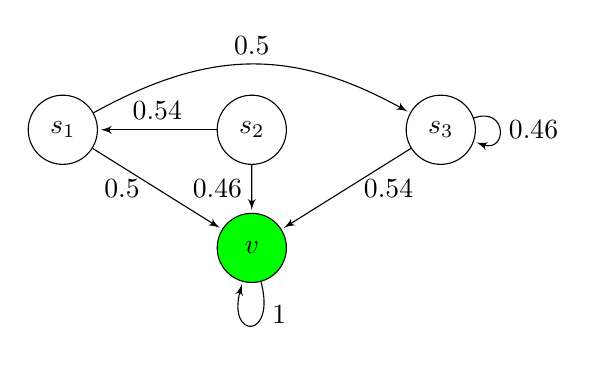
\begin{tikzpicture}[xscale=.6,>=latex',shorten >=1pt,node distance=3cm,on grid,auto]
	
	\node[state] (s) at (-6,0) {$s_1$};
	\node[state] (t) at (-2,0) {$s_2$};
	\node[state] (u) at (2,0) {$s_3$};
	\node[state, fill=green] (v) at (-2,-1.5) {$v$};
	
	\path[->] (s) edge [out=20,in=160] node [midway, above] {$0.5$} (u);
	\path[->] (s) edge node [midway, left, xshift=-0.1cm] {$0.5$} (v);
	
	\path[->] (t) edge node [midway, left] {$0.46$} (v);
	\path[->] (t) edge node [midway, above]  {$0.54$} (s);%[out=160,in=20]
	
	\path[->] (u) edge node [midway, right, xshift=0.1cm] {$0.54$} (v);
	\path[->] (u) edge [loop right] node [midway, right] {$0.46$} (u);
	
	\path[->] (v) edge [out=-70, in=-110, looseness=4] node [near start, right] {$1$} (v);
	\end{tikzpicture}
	\captionof{figure}{The LMC for which Algorithm~\ref{alg:local-distance-merge-algorithm} may perform better than Algorithm~\ref{alg:approximate-partition-refinement-merge-algorithm}.}
	\label{fig:example-local-merging-better}
\end{minipage}
\hfill
\begin{minipage}{0.45\textwidth}
	\centering	\vspace{0.1cm}
	\begin{tabular}{l}
		\\\\\\
		\hline%wd{0.5pt}
		$X_0 = \{S\}$ \\
		$X_1 = \big\{  \{s_1,s_2,s_3\} , \{v\} \big\}$\\
		$X_2 = \big\{  \{s_1, s_2\}, \{s_3\} , \{v\} \big\}$\\
		$X_3 = \big\{  \{s_1\},\{s_2\}, \{s_3\} , \{v\} \big\}$\\
		\hline
		\\\\
	\end{tabular}
	\captionof{table}{Example of running Algorithm~\ref{alg:polynomial-optimistic-partition-refinement} on the LMC in \cref{fig:example-local-merging-better}. (Suppose we iterate through $s_1$ and $s_2$ before $s_3$.)} \label{tab:example-approximate-partition-refinement}
\end{minipage}

\begin{minipage}{0.5\textwidth}
	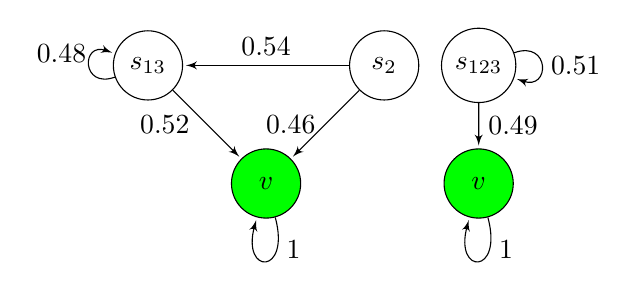
\begin{tikzpicture}[xscale=.6,>=latex',shorten >=1pt,node distance=3cm,on grid,auto]
	
	\node[state] (s13) at (1.5,0) {$s_{13}$};
	\node[state] (s2) at (6.5,0) {$s_2$};
	\node[state, fill=green] (v1) at (4,-1.5) {$v$};
	
	\path[->] (s13) edge node [midway, left, xshift=-0.1cm] {$0.52$} (v1);
	\path[->] (s13) edge [loop left] node [near end, left] {$0.48$} (s13);
	
	\path[->] (s2) edge node [midway, left] {$0.46$} (v1);
	\path[->] (s2) edge node [midway, above]  {$0.54$} (s13);
	
	\path[->] (v1) edge [out=-70, in=-110, looseness=4] node [near start, right] {$1$} (v1);
	
	\node[state] (ss) at (8.5,0) {$s_{123}$};
	\node[state, fill=green] (vv) at (8.5,-1.5) {$v$};
	
	\path[->] (ss) edge node [midway, right] {$0.49$} (vv);
	\path[->] (ss) edge [loop right] node [midway, right] {$0.51$} (ss);
	\path[->] (vv) edge [out=-70, in=-110, looseness=4] node [near start, right] {$1$} (vv);
	
	\end{tikzpicture}
	\captionof{figure}{Two Steps of Running Algorithm~\ref{alg:local-distance-merge-algorithm}.}\label{fig:example-local-merging-better2}
\end{minipage}
\hfill
\begin{minipage}{0.45\textwidth}
	\centering\vspace{0.2cm}
	\begin{tabular}{l}
		\\\\
		\hline%wd{0.5pt}
		$X_0 = \{S\}$ \\
		$X_1 = \big\{  \{s_1,s_3,s_2\} , \{v\} \big\}$\\
		$X_2 = \big\{  \{s_1, s_3\}, \{s_2\} , \{v\} \big\}$\\
		\hline
		\\
	\end{tabular}
	\captionof{table}{Example of running Algorithm~\ref{alg:polynomial-optimistic-partition-refinement} on the LMC in \cref{fig:example-local-merging-better}. (Suppose we iterate through $s_1$ and $s_3$ before $s_2$.)} \label{tab:example-approximate-partition-refinement2}
\end{minipage}


\section{Conclusion}\label{section:conclusion}

We have developed and analysed algorithms for minimising probabilistic systems via approximate bisimulation.
These algorithms are based on $\epsilon$-quotients, a novel yet natural notion of approximate quotients.
We have obtained theoretical bounds on the discrepancy between the minimised and the non-minimised systems.
In our experiments, approximate partition refinement does well in minimising labelled Markov chains with perturbed  transition probabilities,
suggesting that approximate partition refinement is a practical approach for ``recognising'' and exploiting approximate bisimulation.

Future work might consider the following questions: Does approximate minimisation allow for further forms of active learning? Can our techniques be transferred to Markov decision processes?

\bibliography{paper}

\newpage\appendix\label{section:appendix}
\onecolumn


% \tableofcontents{}

% \newpage

\section*{Supplementary Material}
\addcontentsline{toc}{section}{Supplementary Material}


Throughout this discussion, 
we will make frequently use 
of the following standard results
concerning the exponential concentration 
of random variables:

\begin{lemma}[Hoeffding's inequality for independent RVs~\citep{hoeffding1994probability}] Let $Z_1, Z_2, \ldots, Z_n$ be independent bounded random variables with $Z_i \in [a,b]$ for all $i$, then 
    \begin{align*}
        \prob\left( \frac{1}{n} \sum_{i=1}^n (Z_i - \Expo{Z_i}) \ge t \right) \le \exp{\left( -\frac{2nt^2}{(b-a)^2} \right) }
    \end{align*} 
    and 
    \begin{align*}
        \prob\left( \frac{1}{n} \sum_{i=1}^n (Z_i - \Expo{Z_i}) \le -t \right) \le \exp{\left( -\frac{2nt^2}{(b-a)^2} \right) }
    \end{align*} 
    for all $t \ge 0$. 
\end{lemma}

\begin{lemma}[Hoeffding's inequality for sampling with replacement~\citep{hoeffding1994probability}] \label{lem:hoeffding_sampling} Let $\calZ = (Z_1, Z_2, \ldots, Z_N)$ be a finite population of $N$ points with $Z_i \in [a.b]$ for all $i$. Let $X_1, X_2, \ldots X_n$ be a random sample drawn without replacement from $\calZ$. Then for all $t \ge 0$, we have 
    \begin{align*}
        \prob\left( \frac{1}{n} \sum_{i=1}^n (X_i - \mu ) \ge t \right) \le \exp{\left( -\frac{2nt^2}{(b-a)^2} \right) }
    \end{align*} 
    and 
    \begin{align*}
        \prob\left( \frac{1}{n} \sum_{i=1}^n (X_i - \mu ) \le -t \right) \le \exp{\left( -\frac{2nt^2}{(b-a)^2} \right) } \,,
    \end{align*} 
    where $\mu = \frac{1}{N} \sum_{i=1}^{N} Z_i$. 
\end{lemma}

We now discuss one condition that generalizes the exponential concentration to dependent random variables.
\begin{condition}[Bounded difference inequality] \label{cond:BDC} Let $\calZ$ be some set and $\phi: \calZ^n \to \Real$. We say that $\phi$ satisfies the bounded difference assumption if 
there exists $c_1, c_2, \ldots c_n \ge 0$ s.t. for all $i$, we have 
\begin{align*}
    \sup_{Z_1,Z_2, \ldots,Z_n, Z_i^\prime \in \calZ^{n+1} } \abs{\phi (Z_1, \ldots, Z_i, \ldots, Z_n ) - \phi (Z_1, \ldots, Z_i^\prime, \ldots, Z_n ) } \le c_i \,.
\end{align*} 
\end{condition}

\begin{lemma}[McDiarmid’s inequality~\citep{mcdiarmid1989}] \label{lem:McDiarmid} Let $Z_1, Z_2, \ldots, Z_n$ be independent random variables on set $\calZ$ and $\phi : \calZ^n \to \Real$ satisfy bounded difference inequality (\codref{cond:BDC}). Then for all $t>0$, we have 
    \begin{align*}
        \prob\left( \phi(Z_1, Z_2, \ldots, Z_n) - \Expo{\phi(Z_1, Z_2, \ldots, Z_n)} \ge t \right) \le \exp{\left( -\frac{2t^2}{\sum_{i=1}^n c_i^2} \right) } 
    \end{align*} 
    and 
    \begin{align*}
        \prob\left( \phi(Z_1, Z_2, \ldots, Z_n) - \Expo{\phi(Z_1, Z_2, \ldots, Z_n)} \le -t \right) \le \exp{\left( -\frac{2t^2}{\sum_{i=1}^n c_i^2} \right) } \,.
    \end{align*} 
\end{lemma}


\section{Proofs from \secref{sec:ERM_training}}\label{app:proof_erm}

\textbf{Additional notation {} {}} Let $m_1$ be the number of mislabeled points ($\wt S_M$) and $m_2$ be the number of correctly labeled points ($\wt S_C$). Note $m_1 + m_2 = m$. 


\subsection{Proof of \thmref{thm:error_ERM}}


\begin{proof}[Proof of \lemref{lem:fit_mislabeled}] 
    The main idea of our proof is to regard 
    the clean portion of the data 
    ($S \cup \wt S_C$) as fixed.   
    Then, there exists an (unknown) classifier $f^*$ 
    that minimizes the expected risk
    calculated on the (fixed) clean data
    and (random draws of) the mislabeled data $\wt S_M$. 
    % 
    % 
    Formally, 
    \begin{align}
    f^* \defeq \argmin_{f \in \calF} \error_{\widecheck {\calD}} (f) \,, \label{eq:modified_ERM}
    \end{align}
    where $$\widecheck \calD = \frac{n}{m+n} \calS + \frac{m_2}{m+n} \wt \calS_C  + \frac{m_1}{m+n}\calDm \,.$$ 
    Note here that $\widecheck \calD$ is a combination 
    of the \emph{empirical distribution} 
    over correctly labeled data $S \cup \wt S_C$
    and the (population) distribution 
    over mislabeled data $\calDm$.
    Recall that 
    \begin{align}
    \wh f \defeq \argmin_{f \in \calF} \error_{\calS \cup \wt S} (f) \,. \label{eq:orig_ERM}
    \end{align}
    % 
    % 
    Since, $\widehat f$ minimizes 0-1 error 
    on $S \cup \wt S$, using ERM optimality on \eqref{eq:orig_ERM},  
    we have 
    \begin{align}
        \error_{\calS \cup \wt \calS}(\widehat f) \le \error_{
            \calS \cup \wt \calS}(f^*) \,.    \label{eq:step1}
    \end{align}
    Moreover, since $f^*$ is independent of $\wt S_M$, using Hoeffding's bound,
    % \footnote{For a fully rigorous argument,
    % refer to the complete proof in App.~\ref{app:proof_erm}.} 
    we have with probability at least $1-\delta$ that
    \begin{align}
      \error_{\wt \calS_M}(f^*) \le \error_{ \calDm}(f^*) +  \sqrt{\frac{\log(1/\delta)}{2 m_1}} \,. \label{eq:step2} 
    \end{align}
    %$ 
    %for some constant $c_1\le 1/2$. 
    Finally, since $f^*$ is the optimal classifier on $\widecheck \calD$, 
    we have 
    \begin{align}
        \error_{\widecheck \calD}(f^*) \le \error_{\widecheck \calD}(\widehat f) \,. \label{eq:step3}
    \end{align}
    Now to relate \eqref{eq:step1} and \eqref{eq:step3}, we multiply \eqref{eq:step2} by $\frac{m_1}{m+n}$ and add $\frac{n}{m+n} \error_{\calS} (f)  + \frac{m_2}{m+n} \error_{\wt \calS_C} (f)$ both the sides. Hence, 
    we can rewrite \eqref{eq:step2} as follows: 
    \begin{align}
        \error_{\calS \cup \wt\calS}(f^*) \le \error_{ \widecheck \calD}(f^*) +  \frac{m_1}{m+n}\sqrt{\frac{\log(1/\delta)}{2 m_1}} \,. \label{eq:step4} 
    \end{align}
    Now we combine equations \eqref{eq:step1}, \eqref{eq:step4}, and \eqref{eq:step3}, to get 
    \begin{align}
        \error_{\calS \cup \wt \calS}(\wh f) \le \error_{\widecheck \calD}(\wh f) +  \frac{m_1}{m+n}\sqrt{\frac{\log(1/\delta)}{2 m_1}} \,, 
    \end{align}
    which implies 
    \begin{align}
        \error_{ \wt \calS_M}(\wh f) \le \error_{\calDm}(\wh f) + \sqrt{\frac{\log(1/\delta)}{2 m_1}} \,. \label{eq:lemma1_final}
    \end{align}
    Since $\wt S$ is obtained by randomly labeling an unlabeled dataset, we assume $2m_1 \approx m$ \footnote{Formally, with probability at least $1-\delta$, we have  $(m - 2m_1)\le \sqrt{m\log(1/\delta)/2}$.}. Moreover, using $\error_{\calDm} = 1 - \error_{\calD}$ we obtain the desired result.   
    % Combining the above steps and using the fact 
    % that $\error_\calD = 1- \error_{\calDm} $, 
    % we obtain the desired result.
\end{proof}

\begin{proof}[Proof of \lemref{lem:mislabeled_error}]
    Recall $\error_{\wt S} (f) = \frac{m_1}{m} \error_{\wt S_M}(f) + \frac{m_2}{m} \error_{\wt S_C}(f)$. Hence, we have 
    \begin{align}
        2\error_{\wt S}(f) - \error_{\wt S_M}(f) - \error_{\wt S_C}(f) &= \left(\frac{2m_1}{m} \error_{\wt S_M}(f) - \error_{\wt S_M}(f)\right) + \left(\frac{2m_2}{m} \error_{\wt S_C}(f) - \error_{\wt S_C}(f)\right) \\ &= \left(\frac{2m_1}{m} - 1\right) \error_{\wt S_M}(f) + \left(\frac{2m_2}{m} - 1 \right)\error_{\wt S_C} (f) \,.
    \end{align} 
    Since the dataset is labeled uniformly at random, with probability at least $1-\delta$, we have  $\left(\frac{2m_1}{m} - 1\right) \le \sqrt{\frac{\log(1/\delta)}{2m}}$. Similarly, we have with probability at least $1-\delta$, $\left(\frac{2m_2}{m} - 1\right) \le \sqrt{\frac{\log(1/\delta)}{2m}}$. Using union bound, with probability at least $1-\delta$, we have
    % \begin{align}
    %     2\error_{\wt S} - \error_{\wt S_M}(f) - \error_{\wt S_C}(f) \le \sqrt{\frac{\log(2/\delta)}{2m}} \left(\error_{\wt S_M}(f) + \error_{\wt S_C}(f) \right) \le 2\sqrt{\frac{\log(2/\delta)}{2m}} \,. \label{eq:lemma2_final}
    % \end{align}
    \begin{align}
        2\error_{\wt S} - \error_{\wt S_M}(f) - \error_{\wt S_C}(f) \le \sqrt{\frac{\log(2/\delta)}{2m}} \left(\error_{\wt S_M}(f) + \error_{\wt S_C}(f) \right) \,. \label{eq:lemma2_prefinal}
    \end{align}
    With re-arranging $\error_{\wt S_M}(f) + \error_{\wt S_C}(f)$ and using the inequality $ 1- a\le \frac{1}{1+a} $, we have  
    \begin{align}
        2\error_{\wt S} - \error_{\wt S_M}(f) - \error_{\wt S_C}(f) \le 2\error_{\wt \calS} \sqrt{\frac{\log(2/\delta)}{2m}}  \,. \label{eq:lemma2_final}
    \end{align}

    % We obtain the desired result by using 
\end{proof}

\begin{proof}[Proof of \lemref{lem:clear_error}]
% Recall 0-1 error on each point  $(x,y) \in S \cup \wt S$ is given by $\I{ f(x)\ne y}$.
In the set of correctly labeled points $S \cup \wt S_C$, we have $S$ as a random subset of $S \cup \wt S_C$. Hence, using Hoeffding's inequality for sampling without replacement (\lemref{lem:hoeffding_sampling}), we have with probability at least $1-\delta$
\begin{align}
    \error_{\wt \calS_C} (\wh f)- \error_{\calS \cup \wt \calS_C}( \wh f) \le  \sqrt{\frac{\log(1/\delta)}{2m_2}} \,.
\end{align}
Re-writing $\error_{\calS \cup \wt \calS_C}( \wh f)$ as $\frac{m_2}{m_2 + n} \error_{\wt \calS_C }(\wh f) + \frac{n}{m_2 + n} \error_{\calS }(\wh f)$, we have with probability at least $1-\delta$
\begin{align}
   \left(\frac{n}{n+m_2}\right) \left(\error_{\wt \calS_C} (\wh f)- \error_{\calS}( \wh f) \right) \le  \sqrt{\frac{\log(1/\delta)}{2m_2}} \,.
\end{align}
As before, assuming $2m_2 \approx m$, we have with probability at least $1-\delta$ 
\begin{align}
    \error_{\wt \calS_C} (\wh f)- \error_{\calS}( \wh f) \le \left(1+\frac{m_2}{n}\right)  \sqrt{\frac{\log(1/\delta)}{m}} \le \left(1 + \frac{m}{2n}\right) \sqrt{\frac{\log(1/\delta)}{m}} \,. \label{eq:lemma3_final}
\end{align} 
\end{proof}

\begin{proof}[Proof of \thmref{thm:error_ERM}] 
    Having established these core intermediate results, we can now combine above three lemmas to prove the main result. 
    In particular, we bound the population error on clean data ($\error_\calD(\wh f)$) as follows:  
    \begin{enumerate}[(i)]
        \item First, use \eqref{eq:lemma1_final}, to obtain an upper bound on the population error on clean data, i.e., with probability at least $1-\delta/4$, we have
        \begin{align}
            \error_{ \calD} (\wh f) \le 1 - \error_{ \wt \calS_M}(\wh f) + \sqrt{\frac{\log(4/\delta)}{m}} \,. 
        \end{align}
        \item  Second, use \eqref{eq:lemma2_final}, to relate the error on the mislabeled fraction with error on clean portion of randomly labeled data and error on whole randomly labeled dataset, i.e., with probability at least $1-\delta/2$, we have 
        \begin{align}
            - \error_{\wt S_M}(f) \le \error_{\wt S_C}(f) - 2\error_{\wt S}  + 2\error_{\wt S} \sqrt{\frac{\log(4/\delta)}{2m}}  \,. 
        \end{align} 
        \item Finally, use \eqref{eq:lemma3_final} to relate the error on the clean portion of randomly labeled data and error on clean training data, i.e., with probability $1-\delta/4$, we have 
        \begin{align}
            \error_{\wt \calS_C} (\wh f)\le - \error_{\calS}( \wh f) + \left(1 + \frac{m}{2n} \right) \sqrt{\frac{\log(4/\delta)}{m}} \,. 
        \end{align} 
    \end{enumerate}

    Using union bound on the above three steps, we have with probability at least $1-\delta$: 
    \begin{align}
        \error_\calD (\wh f) \le \error_{\calS}(\wh f)   + 1 - 2\error_{\wt \calS}(\wh f)   + \left(\sqrt{2} \error_{\wt S} + 2 + \frac{m}{2n}\right)  \sqrt{\frac{\log(4/\delta)}{m}} \,.
    \end{align}
    % Note that $(1/\sqrt{2} + 2.5)$ is a loose constant. In experiments, we use the ratio $\frac{m}{n}$
    %  the exact error $\error_{\wt \calS}(\wh f)$ 
    % to evaluate R.H.S.    
\end{proof}

\subsection{Proof of \propref{prop:rademacher}}

\begin{proof}[Proof of \propref{prop:rademacher}]
    For a classifier $ f: \calX \to \{-1, 1\}$, we have $1 - 2\,\indict{ f(x) \ne y} = y \cdot f(x)$. Hence, by definition of $\error$, we have 
    \begin{align}
        1 -2\error_{\wt \calS}(f) = \frac{1}{m}\sum_{i=1}^m y_i \cdot f(x_i) \le \sup_{f \in \calF} \, \frac{1}{m} \sum_{i=1}^m y_i \cdot f(x_i)  \,. \label{eq:error_rademacher}
    \end{align}
    Note that for fixed inputs $(x_1, x_2, \ldots, x_m)$ in $\wt S$, $(y_1, y_2, \ldots y_m)$ are random labels. Define $\phi_1 (y_1, y_2, \ldots, y_m) \defeq \sup_{f \in \calF} \, \frac{1}{m} \sum_{i=1}^m y_i \cdot f(x_i)$. We have the following bounded difference condition on $\phi_1$. For all i, 
    \begin{align}
        \sup_{y_1, \ldots y_m, y_i^\prime \in \{-1, 1\}^{m+1} } \abs{ \phi_1 (y_1,\ldots, y_i, \ldots, y_m) - \phi_1 (y_1,\ldots, y_i^\prime, \ldots, y_m)  } \le 1/m \,. \label{cond1_rademacher}
    \end{align} 
    
    Similarly, we define $\phi_2 (x_1, x_2, \ldots, x_m) \defeq \Expt{ y_i \sim_U \{-1, 1\}  }{ \sup_{f \in \calF} \, \frac{1}{m}  \sum_{i=1}^m y_i \cdot f(x_i)}$. We have the following bounded difference condition on $\phi_2$. 
    For all i,
    \begin{align}
        \sup_{x_1, \ldots x_m, x_i^\prime \in \calX^{m+1} } \abs{ \phi_2 (x_1,\ldots, x_i, \ldots, x_m) - \phi_1 (x_1,\ldots, x_i^\prime, \ldots, x_m)  } \le 1/m \,. \label{cond2_rademacher}
    \end{align}
    Using McDiarmid’s inequality (\lemref{lem:McDiarmid}) twice 
    with Condition \eqref{cond1_rademacher} and \eqref{cond2_rademacher}, 
    with probability at least $1-\delta$, we have
    \begin{align}
        \sup_{f \in \calF} \, \frac{1}{m} \sum_{i=1}^m y_i \cdot f(x_i)  - \Expt{x,y}{\sup_{f \in \calF} \, \frac{1}{m} \sum_{i=1}^m y_i \cdot f(x_i) } \le \sqrt{\frac{2\log(2/\delta)}{m}} \,. \label{eq:final_rademacher}
    \end{align} 
    Combining \eqref{eq:error_rademacher} and \eqref{eq:final_rademacher}, we obtain the desired result. 
\end{proof}


\subsection{Proof of \thmref{thm:error_regularized_ERM}}

Proof of \thmref{thm:error_regularized_ERM} follows similar to the proof of \thmref{thm:error_ERM}. Note that the same results in \lemref{lem:fit_mislabeled}, \lemref{lem:mislabeled_error}, and \lemref{lem:clear_error} hold in the regularized ERM case. However, the arguments in the proof of \lemref{lem:fit_mislabeled} change slightly. Hence, we state the lemma for regularized ERM and prove it here for completeness. 

\begin{lemma} \label{lem:lemma1_reg}
    Assume the same setup as \thmref{thm:error_regularized_ERM}. 
    Then for any $\delta >0$, with probability at least  $1-\delta$ 
    over the random draws of mislabeled data $\wt S_M$, we have 
    \begin{align}
        \error_\calD(\widehat f)  \le 1 -\error_{\wt \calS_M}(\widehat f) + \sqrt{\frac{\log(1/\delta)}{m}}\,. 
    \end{align} 
\end{lemma}
\begin{proof}
    The main idea of the proof remains the same, i.e. regard 
    the clean portion of the data 
    ($S \cup \wt S_C$) as fixed.   
    Then, there exists a classifier $f^*$ 
    that is optimal over draws 
    of the mislabeled data $\wt S_M$. 

    
    Formally, 
    \begin{align}
    f^* \defeq \argmin_{f \in \calF} \error_{\widecheck {\calD}} (f)  + \lambda R(f) \,, \label{eq:modified_ERM_reg}
    \end{align}
    where $$\widecheck \calD = \frac{n}{m+n} \calS + \frac{m_1}{m+n} \wt \calS_C  + \frac{m_2}{m+n}\calDm \,.$$ That is, $\widecheck \calD$ a combination of 
    the \emph{empirical distribution} 
    over correctly labeled data $S \cup \wt S_C$
    % in $S\cup \wt S$ 
    and the (population) distribution 
    over mislabeled data $\calDm$.
    Recall that 
    \begin{align}
    \wh f \defeq \argmin_{f \in \calF} \error_{\calS \cup \wt S} (f) + \lambda R(f) \,. \label{eq:orig_ERM_reg}
    \end{align}
    % 
    % 
    Since, $\widehat f$ minimizes 0-1 error 
    on $S \cup \wt S$, using ERM optimality on \eqref{eq:orig_ERM},  
    we have 
    \begin{align}
        \error_{\calS \cup \wt \calS}(\widehat f) + \lambda R(\wh f) \le \error_{
            \calS \cup \wt \calS}(f^*) + \lambda R(f^*) \,.    \label{eq:step1_reg}
    \end{align}
    Moreover, since $f^*$ is independent of $\wt S_M$, using Hoeffding's bound,
    % \footnote{For a fully rigorous argument,
    % refer to the complete proof in App.~\ref{app:proof_erm}.} 
    we have with probability at least $1-\delta$ that
    \begin{align}
      \error_{\wt \calS_M}(f^*) \le \error_{ \calDm}(f^*) +  \sqrt{\frac{\log(1/\delta)}{2 m_1}} \,. \label{eq:step2_reg} 
    \end{align}
    %$ 
    %for some constant $c_1\le 1/2$. 
    Finally, since $f^*$ is the optimal classifier on $\widecheck \calD$, 
    we have 
    \begin{align}
        \error_{\widecheck \calD}(f^*) + \lambda R(f^*) \le \error_{\widecheck \calD}(\widehat f) + \lambda R(\wh f) \,. \label{eq:step3_reg}
    \end{align}
     Now to relate \eqref{eq:step1_reg} and \eqref{eq:step3_reg}, we can re-write the \eqref{eq:step2_reg} as follows: 
    \begin{align}
        \error_{\calS \cup \wt\calS}(f^*) \le \error_{ \widecheck \calD}(f^*) +  \frac{m_1}{m+n}\sqrt{\frac{\log(1/\delta)}{2 m_1}} \,. \label{eq:step4_reg} 
    \end{align}
    After adding $\lambda R(f^*)$ on both sides in \eqref{eq:step4_reg}, we combine equations \eqref{eq:step1_reg}, \eqref{eq:step4_reg}, and \eqref{eq:step3_reg}, to get 
    \begin{align}
        \error_{\calS \cup \wt \calS}(\wh f) \le \error_{\widecheck \calD}(\wh f) +  \frac{m_1}{m+n}\sqrt{\frac{\log(1/\delta)}{2 m_1}} \,, 
    \end{align}
    which implies 
    \begin{align}
        \error_{ \wt \calS_M}(\wh f) \le \error_{\calDm}(\wh f) + \sqrt{\frac{\log(1/\delta)}{2 m_1}} \,. \label{eq:lemma_reg_final}
    \end{align}
    Similar as before, since $\wt S$ is obtained by randomly labeling an unlabeled dataset, we assume 
    $2m_1 \approx m$. Moreover, using $\error_{\calDm} = 1 - \error_{\calD}$ we obtain the desired result. 
\end{proof}
% \begin{proof}[Proof of ]
    
% \end{proof}

\subsection{Proof of \thmref{thm:multiclass_ERM}}

To prove our results in the multiclass case,
we first state and prove lemmas
parallel to those
% We first state and prove lemmas 
% parallel 
% to the three lemmas 
used in the proof of balanced binary case. 
We then combine these results 
% in the three lemmas 
to obtain the result in \thmref{thm:multiclass_ERM}. 

Before stating the result, 
we define mislabeled distribution $\calDm$ for any $\calD$.
While $\calDm$ and $\calD$ share 
the same marginal distribution over inputs $\calX$,
the conditional distribution over labels $y$ 
given an input $x\sim \calD_\calX$ is changed as follows:
For any $x$, the Probability Mass Function (PMF) over $y$ is defined as:  
$p_{\calDm} (\cdot \vert x) \defeq \frac{1 - p_{\calD}(\cdot \vert x)}{k - 1}$, where $ p_{\calD}(\cdot \vert x)$ is the PMF over $y$ for the distribution $\calD$. 

\begin{lemma} \label{lem:fit_mislabeled_multi}
    Assume the same setup as \thmref{thm:multiclass_ERM}. 
    Then for any $\delta >0$, with probability at least  $1-\delta$ 
    over the random draws of mislabeled data $\wt S_M$, we have 
    \begin{align}
        \error_\calD(\widehat f)  \le (k-1)\left(1 -\error_{\wt \calS_M}(\widehat f)\right) + (k-1)\sqrt{\frac{\log(1/\delta)}{m}}\,. \label{eq:lemma1_multi}
    \end{align}   
\end{lemma} 

\begin{proof}
   
    The main idea of the proof remains the same.
    We begin by regarding the clean portion of the data 
    ($S \cup \wt S_C$) as fixed. 
    Then, there exists a classifier $f^*$ 
    that is optimal over draws 
    of the mislabeled data $\wt S_M$. 
    
    However, in the multiclass case,
    we cannot as easily relate the population error on mislabeled data 
    to the population accuracy on clean data.   
    While for binary classification, 
    % we could upper bound $\error_{\wt \calS_M}$ 
    % with $1-\error_\calD$ 
    we could lower bound the population accuracy $1-\error_\calD$
    with the empirical error on mislabeled data $\error_{\wt \calS_M}$ 
    (in the proof of \lemref{lem:fit_mislabeled}), 
    for multiclass classification, 
    error on the mislabeled data 
    and accuracy on the clean data 
    in the population 
    are not so directly related.  
    To establish \eqref{eq:lemma1_multi},
    we break the error on the 
    (unknown) mislabeled data 
    into two parts: one term corresponds 
    to predicting the true label on mislabeled data, 
    and the other corresponds to predicting 
    neither the true label 
    nor the assigned (mis-)label.  
    Finally, we relate these errors to their
    population counterparts to establish \eqref{eq:lemma1_multi}. 
    
    Formally, 
    \begin{align}
    f^* \defeq \argmin_{f \in \calF} \error_{\widecheck {\calD}} (f)  + \lambda R(f) \,, \label{eq:modified_ERM_reg2}
    \end{align}
    where $$\widecheck \calD = \frac{n}{m+n} \calS + \frac{m_1}{m+n} \wt \calS_C  + \frac{m_2}{m+n}\calDm \,.$$ 
    That is, $\widecheck \calD$ is a combination 
    of the \emph{empirical distribution} 
    over correctly labeled data $S \cup \wt S_C$
    % in $S\cup \wt S$ 
    and the (population) distribution 
    over mislabeled data $\calDm$.
    Recall that 
    \begin{align}
    \wh f \defeq \argmin_{f \in \calF} \error_{\calS \cup \wt S} (f) + \lambda R(f) \,. \label{eq:orig_ERM_reg2}
    \end{align}
    % 
    % 
    Following the exact steps from the proof of \lemref{lem:lemma1_reg}, 
    with probability at least $1-\delta$, we have  
    \begin{align}
        \error_{ \wt \calS_M}(\wh f) \le \error_{\calDm}(\wh f) + \sqrt{\frac{\log(1/\delta)}{2 m_1}} \,. \label{eq:lemma1_final_multi_prev}
    \end{align}
    Similar to before, since $\wt S$ is obtained 
    by randomly labeling an unlabeled dataset, 
    we assume 
    $\frac{k}{k-1} m_1 \approx m$. 
    
    Now we will relate $\error_{\calDm} (\wh f)$ with $\error_{\calD}(\wh f)$. 
    Let $y^T$ denote the (unknown) true label 
    for a mislabeled point $(x, y)$ 
    (i.e., label before replacing it with a mislabel). 
    \begin{align*}    
         \Expt{(x, y) \in \sim \calDm}{\indict{ \wh f(x) \ne y }}  &= \underbrace{\Expt{(x, y) \in \sim \calDm}{\indict{ \wh f(x) \ne y \land \wh f(x) \ne y^T}}}_{\RN{1}} \\ &\qquad \qquad + \underbrace{\Expt{(x, y) \in \sim \calDm}{\indict{ \wh f(x) \ne y \land \wh f(x) = y^T}}}_{\RN{2}} \,. \numberthis \label{eq:excess_term}
    \end{align*}
    Clearly, term 2 is one minus the accuracy 
    on the clean unseen data, i.e.,
    \begin{align}
        \RN{2} = 1 - \Expt{{x,y} \sim \calD}{ \indict{ \wh f(x) \ne y}} = 1- \error_{\calD}(\wh f) \,. \label{eq:term1}    
    \end{align}
    Next, we relate term 1 with the error on the unseen clean data. 
    We show that term 1 is equal to the error on the unseen clean data 
    scaled by $\frac{k-2}{k-1}$,
    where $k$ is the number of labels.
    Using the definition of mislabeled distribution $\calDm$,  
    we have 
    \begin{align}
        \RN{1} = \frac{1}{k-1} \left( \Expt{(x, y) \in \sim \calD}{ \sum_{i \in \calY \land i\ne y}  \indict{ \wh f(x) \ne i \land \wh f(x) \ne y}} \right) = \frac{k-2}{k-1} \error_{\calD}(\wh f) \,.\label{eq:term2}
    \end{align}    

    Combining the result in \eqref{eq:term1}, \eqref{eq:term2} and \eqref{eq:excess_term}, we have 
    \begin{align}
        \error_{\calDm}(\wh f) = 1- \frac{1}{k-1} \error_{\calD}(\wh f) \,.\label{eq:combine_terms}
    \end{align}
    Finally, combining the result in \eqref{eq:combine_terms} 
    with equation \eqref{eq:lemma1_final_multi_prev}, 
    we have with probability $1-\delta$, 
    \begin{align}
      \error_{\calD}(\wh f) \le  (k-1) \left( 1- \error_{ \wt \calS_M}(\wh f) \right)  + (k-1) \sqrt{\frac{k \log(1/\delta)}{ 2(k-1)m}} \,. \label{eq:lemma1_final_multi}
    \end{align}
\end{proof}

\begin{lemma} \label{lem:mislabeled_error_multi}
    Assume the same setup as \thmref{thm:multiclass_ERM}. 
    Then for any $\delta >0$, 
    with probability at least $1-\delta$ 
    over the random draws of $\wt S$, we have  
    % \begin{align}
        $$\abs{k\error_{\wt \calS}(\widehat f) - \error_{\wt \calS_C}(\widehat f) -  (k-1)\error_{\wt \calS_M}(\widehat f) } \le  2k\sqrt{\frac{\log(4/\delta)}{2m}}\,. $$ % \label{eq:lemma2}
    % \end{align}   
    %  for some constant $c_3 \le 1.0\,$.
\end{lemma} 


\begin{proof}
    Recall $\error_{\wt S} (f) = \frac{m_1}{m} \error_{\wt S_M}(f) + \frac{m_2}{m} \error_{\wt S_C}(f)$. Hence, we have 
    \begin{align*}
        k\error_{\wt S}(f) - (k-1)\error_{\wt S_M}(f) - \error_{\wt S_C}(f) &= (k-1)\left(\frac{k m_1}{(k-1) m} \error_{\wt S_M}(f) - \error_{\wt S_M}(f)\right) \\ & \qquad \qquad + \left(\frac{km_2}{m} \error_{\wt S_C}(f) - \error_{\wt S_C}(f)\right) \\ &= k \left[ \left(\frac{m_1}{m} - \frac{k-1}{k}\right) \error_{\wt S_M}(f) + \left(\frac{m_2}{m} - \frac{1}{k} \right) \error_{\wt S_C} (f) \right] \,.
    \end{align*} 
    Since the dataset is randomly labeled, 
    we have with probability at least $1-\delta$, 
    $\left(\frac{m_1}{m} - \frac{k-1}{k}\right) \le \sqrt{\frac{\log(1/\delta)}{2m}}$. 
    Similarly, we have with probability at least $1-\delta$, 
    $\left(\frac{m_2}{m} - \frac{1}{k}\right) \le \sqrt{\frac{\log(1/\delta)}{2m}}$. 
    Using union bound, we have with probability at least $1-\delta$
    % \begin{align}
    %     2\error_{\wt S} - \error_{\wt S_M}(f) - \error_{\wt S_C}(f) \le \sqrt{\frac{\log(2/\delta)}{2m}} \left(\error_{\wt S_M}(f) + \error_{\wt S_C}(f) \right) \le 2\sqrt{\frac{\log(2/\delta)}{2m}} \,. \label{eq:lemma2_final}
    % \end{align}
    \begin{align}
        k\error_{\wt S}(f) - (k-1)\error_{\wt S_M}(f) - \error_{\wt S_C}(f)  \le k \sqrt{\frac{\log(2/\delta)}{2m}} \left(\error_{\wt S_M}(f) + \error_{\wt S_C}(f) \right) \,. \label{eq:lemma2_final_multi}
    \end{align}

    % We obtain the desired result by using 
\end{proof}

\begin{lemma} \label{lem:clear_error_multi}
    Assume the same setup as \thmref{thm:multiclass_ERM}. 
    Then for any $\delta >0$, with probability at least $1-\delta$ 
    over the random draws of $\wt S_C$ and $S$, we have 
    % \begin{align}
        $$\abs{\error_{\wt \calS_C}(\widehat f) - \error_{\calS}(\widehat f) } \le 1.5 \sqrt{\frac{k\log(2/\delta)}{2m}}\,.$$ %\label{eq:lemma3}
    % \end{align}   
    % for some constant $c_2 \le 1.2\,$.
\end{lemma} 
\begin{proof}
    % Recall 0-1 error on each point  $(x,y) \in S \cup \wt S$ is given by $\I{ f(x)\ne y}$.
    In the set of correctly labeled points $S \cup \wt S_C$,
    we have $S$ as a random subset of $S \cup \wt S_C$. 
    Hence, using Hoeffding's inequality 
    for sampling without replacement 
    (\lemref{lem:hoeffding_sampling}), 
    we have with probability at least $1-\delta$
    \begin{align}
        \error_{\wt \calS_c} (\wh f)- \error_{\calS \cup \wt \calS_C}( \wh f) \le  \sqrt{\frac{\log(1/\delta)}{2m_2}} \,.
    \end{align}
    Re-writing $\error_{\calS \cup \wt \calS_C}( \wh f)$ 
    as $\frac{m_2}{m_2 + n} \error_{\wt \calS_C }(\wh f) + \frac{n}{m_2 + n} \error_{\calS }(\wh f)$, 
    we have with probability at least $1-\delta$
    \begin{align}
       \left(\frac{n}{n+m_2}\right) \left(\error_{\wt \calS_c} (\wh f)- \error_{\calS}( \wh f) \right) \le  \sqrt{\frac{\log(1/\delta)}{2m_2}} \,.
    \end{align}
    As before, assuming $km_2 \approx m$, 
    we have with probability at least $1-\delta$ 
    \begin{align}
        \error_{\wt \calS_c} (\wh f)- \error_{\calS}( \wh f) \le \left(1+\frac{m_2}{n}\right)  \sqrt{\frac{k\log(1/\delta)}{2m}} \le \left( 1 + \frac{1}{k}\right) \sqrt{\frac{k\log(1/\delta)}{2m}} \,. \label{eq:lemma3_final_multi}
    \end{align} 
\end{proof}

\begin{proof}[Proof of \thmref{thm:multiclass_ERM}] 
    Having established these core intermediate results, 
    we can now combine above three lemmas. 
    In particular, we bound the population error 
    on clean data ($\error_\calD(\wh f)$) as follows:  
    \begin{enumerate}[(i)]
        \item First, use \eqref{eq:lemma1_final_multi}, 
        to obtain an upper bound on the population error on clean data, 
        i.e., with probability at least $1-\delta/4$, we have
        \begin{align}
            \error_{ \calD} (\wh f) \le (k-1)\left(1 - \error_{ \wt \calS_M}(\wh f) \right) + (k-1) \sqrt{\frac{k\log(4/\delta)}{2(k-1)m}} \,. 
        \end{align}
        \item  Second, use \eqref{eq:lemma2_final_multi}
        to relate the error on the mislabeled fraction 
        with error on clean portion of randomly labeled data 
        and error on whole randomly labeled dataset, 
        i.e., with probability at least $1-\delta/2$, we have 
        \begin{align}
            - (k-1)\error_{\wt S_M}(f) \le \error_{\wt S_C}(f) - k\error_{\wt S}  + k\sqrt{\frac{\log(4/\delta)}{2m}}  \,. 
        \end{align} 
        \item Finally, use \eqref{eq:lemma3_final_multi} 
        to relate the error on the clean portion of randomly labeled data 
        and error on clean training data, 
        i.e., with probability $1-\delta/4$, we have 
        \begin{align}
            \error_{\wt \calS_C} (\wh f)\le - \error_{\calS}( \wh f) + \left(1 + \frac{m}{kn} \right) \sqrt{\frac{k\log(4/\delta)}{2m}} \,. 
        \end{align} 
    \end{enumerate}

    Using union bound on the above three steps, 
    we have with probability at least $1-\delta$: 
    \begin{align}
        \error_\calD (\wh f) \le \error_{\calS}(\wh f) + (k-1) - k\error_{\wt \calS}(\wh f)   + (\sqrt{k(k-1)} + k + \sqrt{k} + \frac{m}{n\sqrt{k}})  \sqrt{\frac{\log(4/\delta)}{2m}} \,.\label{eq:multiclass_ERM_final}
    \end{align}
    Simplifying the term in RHS of \eqref{eq:multiclass_ERM_final}, 
    we get the desired result. 
    % Note that since $\frac{m}{n\sqrt{k}}$ 
    % is much smaller than the sum of the other terms
    % the other terms in summation, 
    % we ignore $\frac{m}{n\sqrt{k}}$  
    % Z: ??? --- great
    % that 
    % them
    in the final bound. 
    % we ignore that in the final bound. 
    % Note that $(1/\sqrt{2} + 2.5)$ is a loose constant. In experiments, we use the ratio $\frac{m}{n}$
    %  the exact error $\error_{\wt \calS}(\wh f)$ 
    % to evaluate R.H.S.    
\end{proof}

\newpage
\section{Proofs from \secref{sec:linear_models}}\label{app:proof_gd}
We suppose that the parameters of the linear function 
are obtained via gradient descent on 
the following $L_2$ regularized problem: 
\begin{align}
    % n in denominator is avoided deliberately
    \calL_S(w; \lambda) \defeq \sum_{i=1}^n{(w^Tx_i - y_i)^2} + \lambda \norm{w}{2}^2 \,, \label{eq:l2_MSE_app}   
\end{align}
where $\lambda\ge0$ is a regularization parameter. 
We assume access to a clean dataset 
$S = \{(x_i, y_i)\}_{i=1}^n \sim \calD^n$ 
and randomly labeled dataset 
$\wt S = \{(x_i, y_i)\}_{i=n+1}^{n+m} \sim \wt \calD^m$. 
Let $\bX = [x_1, x_2, \cdots, x_{m+n}]$ 
and $\by = [y_1, y_2, \cdots, y_{m+n}]$. 
Fix a positive learning rate $\eta$ such that 
$\eta \le 1/\left(\norm{\bX^T\bX}{\text{op}} + \lambda^2\right)$ 
and an initialization $w_0 = 0$. 
% \todos{Assumption made for simplicty}. 
Consider the following gradient descent iterates 
to minimize objective \eqref{eq:l2_MSE_app} on $S \cup \wt S$:
\begin{align}
w_t = w_{t-1} - \eta \grad_w \calL_{S \cup \wt S} (w_{t-1}; \lambda) \quad \forall t=1,2,\ldots \label{eq:GD_iterates_app}
\end{align} 
Then we have $\{ w_t\}$ converge to the limiting solution 
$\wh w = \left( \bX^T\bX+\lambda \boldsymbol{I}\right)^{-1}\bX^T\by$. Define $\widehat f (x) \defeq f(x ; \wh w) $.  

% \subsection{\textcolor{red}{Errata}}

% We wish to correct the following error in the body:
% \codref{cond:error_stability} is not enough 
% to guarantee the result in \thmref{thm:linear}. 
% We now present a slightly stronger condition 
% called \emph{hypothesis stability} 
% under which we obtain a result 
% similar to \thmref{thm:linear}. 

% This error doesn't change the main arguments of the proof,
% where we show that the empirical train error 
% is less than or equal to the leave-one-out error.
% We need a stronger condition to relate leave-one-out error 
% with the population error of the original classifier. 
% Specifically, while \codref{cond:error_stability} 
% relates the average population error of leave-one-out classifiers 
% with the population error of the original classifier, 
% we need the new condition to show the concentration 
% of the empirical leave-one-out error 
% and average population error of leave-one-out classifiers. 
% main takeaway 

% Note that the new condition, 
% while being stronger than the previous one, 
% still doesn't imply generalization \citep{bousquet2002stability,elisseeff2003leave,abou2019exponential}. 
% Overall, the main results in \secref{sec:ERM_training} 
% and takeaways of the paper remain unaffected by the error.  

% We now present the new condition 
% and a corrected statement of \thmref{thm:linear}. 
% Recall, for a given training set $S \sim \calD^n $, 
% we use $S_{(i)}$ to denote the training set $S$ 
% with the $i^{\text{th}}$ point removed.

% \begin{condition}[Hypothesis Stability] 
%     \label{cond:hypothesis_stability}
%     We have $\beta$ hypothesis stability 
%     if our training algorithm $\calA$ satisfies the following: 
%     \begin{align*}
%     % ${\sum_{i=1}^n \frac{\error_{\calD}( f(\calA, S_{(i)}))}{n} - \error_\calD(f(\calA, S))} \le \beta\,$.
%     \forall i \in \{1,2,\ldots, n\}, \quad  \Expt{\calS, (x,y) \in \calD}{ \abs{\error\left( f(x) ,y  \right) - \error\left( f_{(i)}(x), y \right) }} \le \frac{\beta}{n} \,,
%     \end{align*}
%     where $f_{(i)} \defeq f(\calA, S_{(i)})$ and $ f \defeq f(\calA, S)$.
% \end{condition}

% \begin{theorem}[Correct statement of \thmref{thm:linear}] \label{thm:new_linear}
%     Assume that this gradient descent algorithm satisfies \codref{cond:hypothesis_stability}
%     with $\beta=\calO(1)$.  
%     Then for any $\delta >0$, with probability at least $1-\delta$ 
%     over the random draws of datasets $\wt S$ and $S$, we have:
%     \begin{align}
%         \error_\calD(\widehat f) \le \error_\calS(\widehat f) + 1 - 2 \error_{\wt\calS}(\widehat f) + \left(\frac{1}{\sqrt{2}} + 1.5 \right) \sqrt{\frac{\log(4/\delta)}{m}} + \sqrt{\frac{4}{\delta}\left(\frac{1}{m} +\frac{3\beta}{m+n} \right)}  \,. \label{eq:gd_error}
%     \end{align} 
%     % for some constant $c\le 3.2$.
% \end{theorem}

\subsection{Proof of \thmref{thm:linear}}
We use a standard result from linear algebra, 
namely the Shermann-Morrison formula 
\citep{sherman1950adjustment} for matrix inversion:  

\begin{lemma}[\citet{sherman1950adjustment}] \label{lem:sherman}
    Suppose $\bA \in \Real^{n \times n}$ 
    is an invertible square matrix 
    and $u,v \in \Real^n$ are column vectors. 
    Then $\bA + uv^T$ is invertible iff $1 + v^T \bA u \ne 0$ 
    and in particular
    \begin{align}
        (\bA + u v^T)^{-1} = \bA^{-1}  - \frac{\bA^{-1} uv^T \bA^{-1} }{ 1 + v^T \bA^{-1} u} \,.
    \end{align}   
\end{lemma}
\newcommand\byy[1]{\by_{\left(#1\right)}}
\newcommand\bXX[1]{\bX_{\left(#1\right)}}
\newcommand\ff[1]{\wh f_{\left(#1\right)}}

For a given training set $S \cup \wt S_C$, 
define leave-one-out error 
on mislabeled points in the training data 
as $$\error_{\text{LOO}(\wt S_M) } = \frac{\sum_{(x_i, y_i) \in \wt S_M} \error( f_{(i)}( x_i), y_i)}{ \abs{\wt S_M }} \,, $$
where $f_{(i)} \defeq f(\calA, (S \cup \wt S)_{(i)})$. 
To relate empirical leave-one-out error and population error 
with hypothesis stability condition, 
we use the following lemma:   

\begin{lemma}[\citet{bousquet2002stability}] \label{lem:stability_error}
    For the leave-one-out error, we have
    \begin{align}
        \Expo{ \left( \error_{\calDm}(\wh f) -\error_{\text{LOO}(\wt S_M) } \right)^2 } \le \frac{1}{2m_1}+  \frac{3\beta}{n + m}\,.
    \end{align}   
    % where $ f \defeq f(\calA, S \cup \wt S) $.
\end{lemma}

Proof of the above lemma is similar 
to the proof of Lemma 9 in \citet{bousquet2002stability} 
and can be found in \appref{app:proof_lem_error}. 
% 
% Before presenting the result, we introduce some notation. 
Before presenting the proof of \thmref{thm:linear}, 
we introduce some more notation. 
Let $\bX_{(i)}$ denote the matrix of covariates 
with the $i^{\text{th}}$ point removed. 
Similarly, let $\by_{(i)}$ be the array of responses 
with the $i^{\text{th}}$ point removed. 
Define the corresponding regularized GD solution 
as $\wh w_{(i)} = \left( \bXX{i}^T\bXX{i}+\lambda \boldsymbol{I}\right)^{-1}\bXX{i}^T\byy{i}$. 
Define $\ff{i}(x) \defeq f(x ; \wh w_{(i)}) $.

\begin{proof}[Proof of \thmref{thm:linear}]
    Because squared loss minimization does not imply 0-1 error minimization, 
    we cannot use arguments from \lemref{lem:fit_mislabeled}. 
    This is the main technical difficulty. 
    To compare the 0-1 error at a train point with an unseen point, 
    we use the closed-form expression for $\widehat{w}$ 
    and Shermann-Morrison formula 
    to upper bound training error 
    with leave-one-out cross validation error. 
    
    The proof is divided into three parts: 
    In part one, we show that 0-1 error 
    on mislabeled points in the training set 
    is lower than the error obtained 
    by leave-one-out error at those points. 
    In part two, we relate this leave-one-out error 
    with the population error on mislabeled distribution
    using \codref{cond:hypothesis_stability}.
    While the empirical leave-one-out error is an unbiased estimator 
    of the average population error of leave-one-out classifiers, 
    we need hypothesis stability 
    to control the variance 
    of empirical leave-one-out error. 
    Finally, in part three, we show 
    that the error on the mislabeled training points 
    can be estimated with just the randomly labeled 
    and clean training data (as in proof of \thmref{thm:error_ERM}).  

    \textbf{Part 1 {} {}} First we relate training error with leave-one-out error.        
    For any training point $(x_i, y_i)$ in $\wt S \cup S$, we have 
    \begin{align}
        \error(\wh f(x_i), y_i ) &= \indict{ y_i \cdot x_i^T \wh w < 0 } = \indict{ y_i \cdot x_i^T \left( \bX^T\bX+\lambda \boldsymbol{I}\right)^{-1}\bX^T\by < 0 } \\
        &= \indict{ y_i \cdot x_i^T \underbrace{\left( \bXX{i}^T\bXX{i} + x_i ^T x_i +\lambda \boldsymbol{I}\right)^{-1}}_{\RN{1}} (\bXX{i}^T\byy{i} + y_i \cdot x_i) < 0 } \,.
    \end{align}
    Letting $\bA = \left(\bXX{i}^T\bXX{i} +\lambda \boldsymbol{I}\right)$ 
    and using \lemref{lem:sherman} on term 1, we have 
    \begin{align}
        \error(\wh f(x_i), y_i ) &= \indict{ y_i \cdot x_i^T \left[\bA^{-1} -  \frac{\bA^{-1} x_i x_i^T \bA^{-1}}{ 1 + x_i ^T \bA^{-1} x_i } \right] (\bXX{i}^T\byy{i} + y_i \cdot x_i) < 0 } \\
        &= \indict{ y_i \cdot\left[ \frac{ x_i^T \bA^{-1} ( 1 + x_i ^T \bA^{-1} x_i ) -  x_i^T \bA^{-1} x_i x_i^T \bA^{-1}}{ 1 + x_i ^T \bA ^{-1}x_i } \right] (\bXX{i}^T\byy{i} + y_i \cdot x_i) < 0 } \\
        &= \indict{ y_i \cdot\left[ \frac{ x_i^T \bA^{-1}}{ 1 + x_i ^T \bA ^{-1}x_i } \right] (\bXX{i}^T\byy{i} + y_i \cdot x_i) < 0 } \,.
    \end{align}

    Since $1 + x_i^T \bA^{-1} x_i > 0$, we have 
    \begin{align}
        \error(\wh f(x_i), y_i ) &= \indict{ y_i \cdot x_i^T \bA^{-1} (\bXX{i}^T\byy{i} + y_i \cdot x_i) < 0 } \\
        &= \indict{ x_i^T \bA^{-1} x_i +  y_i \cdot x_i^T \bA^{-1} (\bXX{i}^T\byy{i}) < 0 } \\
        &\le \indict{ y_i \cdot x_i^T \bA^{-1} (\bXX{i}^T\byy{i}) < 0 } = \error(\ff{i}(x_i), y_i ) \,.\label{eq:LOO_error}
    \end{align}

    Using \eqref{eq:LOO_error}, we have 
    \begin{align}
        \error_{\wt \calS_M } (\wh f) \le \error_{\text{LOO} (\wt S_M)} \defeq \frac{\sum_{(x_i, y_i) \in \wt S_M} \error(\ff{i}(x_i), y_i ) }{\abs{\wt \calS_M}}\label{eq:LOO_error_final} \,.
    \end{align}
    \textbf{Part 2 {}{}} We now relate RHS in \eqref{eq:LOO_error_final} 
    with the population error on mislabeled distribution. 
    To do this, we leverage \codref{cond:hypothesis_stability} 
    and \lemref{lem:stability_error}. 
    In particular, we have 

    \begin{align}
        \Expt{\calS \cup \wt \calS_M }{ \left(\error_{\calDm}(\wh f) - \error_{\text{LOO} (\wt S_M)}\right)^2 } \le \frac{1}{2m_1} + \frac{3\beta}{m+n} \,.
    \end{align}

    Using Chebyshev's inequality, with probability at least $1-\delta$, we have 
    \begin{align}
        \error_{\text{LOO} (\wt S_M)} \le  \error_{\calDm}(\wh f)   + \sqrt{\frac{1}{\delta}\left(\frac{1}{2m_1} +\frac{3\beta}{m+n} \right)} \,. \label{eq:final_mislabeled_linear}
    \end{align}
    

    \textbf{Part 3 {}{}} Combining \eqref{eq:final_mislabeled_linear} and \eqref{eq:LOO_error_final}, we have 

    \begin{align}
        \error_{\wt \calS_M } (\wh f) \le \error_{\calDm}(\wh f)   + \sqrt{\frac{1}{\delta}\left(\frac{1}{2m_1} +\frac{3\beta}{m+n} \right)} \,. \label{eq:linear_parallel_lem1}
    \end{align}

    Compare \eqref{eq:linear_parallel_lem1} with \eqref{eq:lemma1_final} 
    in the proof of \lemref{lem:fit_mislabeled}. 
    We obtain a similar relationship 
    between $\error_{\wt \calS_M }$ and $\error_{\calDm}$ 
    but with a polynomial concentration 
    instead of exponential concentration. 
    In addition, since we just use concentration arguments 
    to relate mislabeled error to the errors
    on the clean and unlabeled portions 
    of the randomly labeled data, 
    we can directly use the results 
    in \lemref{lem:mislabeled_error} and \lemref{lem:clear_error}. 
    Therefore, combining results in \lemref{lem:mislabeled_error}, \lemref{lem:clear_error}, and \eqref{eq:linear_parallel_lem1} with union bound, 
    we have with probability at least $1-\delta$
    \begin{align}
        \error_\calD(\widehat f) \le \error_\calS(\widehat f) + 1 - 2 \error_{\wt\calS}(\widehat f) + \left(\sqrt{2}\error_{\wt\calS}(\widehat f) + 1 + \frac{m}{2n} \right) \sqrt{\frac{\log(4/\delta)}{m}} + \sqrt{\frac{4}{\delta}\left(\frac{1}{m} +\frac{3\beta}{m+n} \right)}  \,.
    \end{align}
    

       
\end{proof}

\subsection{Extension to multiclass classification} \label{app:multiclass_linear}
For multiclass problems with squared loss minimization, as standard practice, we consider one-hot encoding for the underlying label, i.e., a class label $c \in [k]$ is treated as $(0, \cdot, 0,1,0, \cdot, 0) \in \Real^k$ (with $c$-th coordinate being 1).  As before, we suppose that the parameters of the linear function 
are obtained via gradient descent on the following $L_2$ regularized problem: 
\begin{align}
    % n in denominator is avoided deliberately
    \calL_S(w; \lambda) \defeq \sum_{i=1}^n\norm{w^Tx_i - y_i}{2}^2 + \lambda \sum_{j=1}^k \norm{w_j}{2}^2 \,, \label{eq:l2_multiclass_MSE_app}   
\end{align}
where $\lambda\ge0$ is a regularization parameter. 
We assume access to a clean dataset 
$S = \{(x_i, y_i)\}_{i=1}^n \sim \calD^n$ 
and randomly labeled dataset 
$\wt S = \{(x_i, y_i)\}_{i=n+1}^{n+m} \sim \wt \calD^m$. 
Let $\bX = [x_1, x_2, \cdots, x_{m+n}]$ 
and $\by = [e_{y_1}, e_{y_2}, \cdots, e_{y_{m+n}}]$. 
Fix a positive learning rate $\eta$ such that 
$\eta \le 1/\left(\norm{\bX^T\bX}{\text{op}} + \lambda^2\right)$ 
and an initialization $w_0 = 0$. 
% \todos{Assumption made for simplicty}. 
Consider the following gradient descent iterates 
to minimize objective \eqref{eq:l2_MSE_app} on $S \cup \wt S$:
\begin{align}
{w_j}^t = {w_j}^{t-1} - \eta \grad_{w_j} \calL_{S \cup \wt S} (w^{t-1}; \lambda) \quad \forall t=1,2,\ldots \text{ and } j=1,2,\ldots,k  \,. \label{eq:GD_multi_iterates_app}
\end{align} 
Then we have $\{ {w_j}^t\}$ for all $j =1,2,\cdots, k$ converge to the limiting solution 
$\wh w_j = \left( \bX^T\bX+\lambda \boldsymbol{I}\right)^{-1}\bX^T\by_j$. Define $\widehat f (x) \defeq f(x ; \wh w) $.  

\begin{theorem}\label{thm:multi_linear}
    Assume that this gradient descent algorithm satisfies \codref{cond:hypothesis_stability}
    with $\beta=\calO(1)$.  
    Then for a multiclass classification problem wth $k$ classes, for any $\delta >0$, with probability at least $1-\delta$, we have:
    \begin{align*}
        \error_\calD(\widehat f) \le \error_\calS(\widehat f) &+ (k-1)\left(1 - \frac{k}{k-1} \error_{\wt\calS}(\widehat f) \right) \\ &+ \left(k + \sqrt{k} + \frac{m}{n\sqrt{k}} \right) \sqrt{\frac{\log(4/\delta)}{2m}} + \sqrt{k(k-1)} \sqrt{\frac{4}{\delta}\left(\frac{1}{m} +\frac{3\beta}{m+n} \right)}  \,. \numberthis \label{eq:gd_multi_error}
    \end{align*} 
    % for some constant $c\le 3.2$.
\end{theorem}
\begin{proof}
    The proof of this theorem is divided into two parts. In the first part, we relate the error on the mislabeled samples with the population error on the mislabeled data. Similar to the proof of \thmref{thm:linear}, we use Shermann-Morrison formula to upper bound training error with leave-one-out error on each $\wh w^j$. Second part of the proof follows entirely from the proof of \thmref{thm:multiclass_ERM}. In essence, the first part derives an equivalent of \eqref{eq:lemma1_final_multi_prev} for GD training with squared loss and then the second part follows from the proof  of \thmref{thm:multiclass_ERM}. 
    
    \textbf{Part-1:} Consider a training point $(x_i,y_i)$ in $\wt S \cup S $. For simplicity, we use $c_i$ to denote the class of $i$-th point and use $y_i$ as the corresponding one-hot embedding. Recall error in multiclass point is given by $\error(\wh f(x_i), y_i ) = \indict{ c_i \not \in \argmax x_i^T \wh w }$. Thus, there exists a $j \ne c_i \in [k]$, such that we have
     \begin{align}
        \error(\wh f(x_i), y_i ) &= \indict{ c_i \not \in \argmax x_i^T \wh w } = \indict{ x_i^T \wh w_{c_i} < x_i^T \wh w_{j}  } \\ &= \indict{ x_i^T \left( \bX^T\bX+\lambda \boldsymbol{I}\right)^{-1}\bX^T\by_{c_i} < x_i^T \left( \bX^T\bX+\lambda \boldsymbol{I}\right)^{-1}\bX^T\by_{j} } \\
        &= \indict{ x_i^T \underbrace{\left( \bXX{i}^T\bXX{i} + x_i ^T x_i +\lambda \boldsymbol{I}\right)^{-1}}_{\RN{1}} \left(\bXX{i}^T{\by_{c_i}}_{(i)} + x_i - \bXX{i}^T{\by_{j}}_{(i)}\right) < 0 } \,.
    \end{align}
    Letting $\bA = \left(\bXX{i}^T\bXX{i} +\lambda \boldsymbol{I}\right)$ 
    and using \lemref{lem:sherman} on term 1, we have 
    \begin{align}
        \error(\wh f(x_i), y_i ) &= \indict{ x_i^T \left[\bA^{-1} -  \frac{\bA^{-1} x_i x_i^T \bA^{-1}}{ 1 + x_i ^T \bA^{-1} x_i } \right]  \left(\bXX{i}^T{\by_{c_i}}_{(i)} + x_i - \bXX{i}^T{\by_{j}}_{(i)}\right) < 0 } \\
        &= \indict{ \left[ \frac{ x_i^T \bA^{-1} ( 1 + x_i ^T \bA^{-1} x_i ) -  x_i^T \bA^{-1} x_i x_i^T \bA^{-1}}{ 1 + x_i ^T \bA ^{-1}x_i } \right]  \left(\bXX{i}^T{\by_{c_i}}_{(i)} + x_i - \bXX{i}^T{\by_{j}}_{(i)}\right) < 0 } \\
        &= \indict{ \left[ \frac{ x_i^T \bA^{-1}}{ 1 + x_i ^T \bA ^{-1}x_i } \right]  \left(\bXX{i}^T{\by_{c_i}}_{(i)} + x_i - \bXX{i}^T{\by_{j}}_{(i)}\right) < 0} \,.
    \end{align}
    Since $1 + x_i^T \bA^{-1} x_i > 0$, we have 
    \begin{align}
        \error(\wh f(x_i), y_i ) &= \indict{ x_i^T \bA^{-1}  \left(\bXX{i}^T{\by_{c_i}}_{(i)} + x_i - \bXX{i}^T{\by_{j}}_{(i)}\right) < 0 } \\
        &= \indict{ x_i^T \bA^{-1} x_i +  x_i^T \bA^{-1}  \bXX{i}^T{\by_{c_i}}_{(i)}  - x_i^T\bA^{-1}  \bXX{i}^T{\by_{j}}_{(i)} < 0 } \\
        &\le \indict{  x_i^T \bA^{-1}  \bXX{i}^T{\by_{c_i}}_{(i)}  - x_i^T\bA^{-1}  \bXX{i}^T{\by_{j}}_{(i)} < 0  } = \error(\ff{i}(x_i), y_i ) \,.\label{eq:LOO_error_multi}
    \end{align}
    Using \eqref{eq:LOO_error_multi}, we have 
    \begin{align}
        \error_{\wt \calS_M } (\wh f) \le \error_{\text{LOO} (\wt S_M)} \defeq \frac{\sum_{(x_i, y_i) \in \wt S_M} \error(\ff{i}(x_i), y_i ) }{\abs{\wt \calS_M}}\label{eq:LOO_error_multi_final} \,.
    \end{align}
    
    We now relate RHS in \eqref{eq:LOO_error_final} 
    with the population error on mislabeled distribution. 
    Similar as before, to do this, we leverage \codref{cond:hypothesis_stability} 
    and \lemref{lem:stability_error}. Using  \eqref{eq:final_mislabeled_linear} and \eqref{eq:LOO_error_multi_final}, we have 
    \begin{align}
        \error_{\wt \calS_M } (\wh f) \le \error_{\calDm}(\wh f)   + \sqrt{\frac{1}{\delta}\left(\frac{1}{2m_1} +\frac{3\beta}{m+n} \right)} \,. \label{eq:linear_multi_parallel_lem1}
    \end{align}
    
    We have now derived a parallel to \eqref{eq:lemma1_final_multi_prev}. Using the same arguments in the proof of \lemref{lem:fit_mislabeled_multi}, we have 
    \begin{align}
      \error_{\calD}(\wh f) \le  (k-1) \left( 1- \error_{ \wt \calS_M}(\wh f) \right)  + (k-1)\sqrt{\frac{k}{\delta(k-1)}\left(\frac{1}{2m_1} +\frac{3\beta}{m+n} \right)}  \,. \label{eq:lemma1_linear_final_multi}
    \end{align}
    
    \textbf{Part-2:} We now combine the results in \lemref{lem:mislabeled_error_multi} and \lemref{lem:clear_error_multi} to obtain the final inequality in terms of quantities that can be computed from just the randomly labeled and clean data. Similar to the binary case, we obtained a polynomial concentration instead of exponential concentration. Combining \eqref{eq:lemma1_linear_final_multi} with \lemref{lem:mislabeled_error_multi} and \lemref{lem:clear_error_multi}, we have with probability at least $1-\delta$
    \begin{align*}
        \error_\calD(\widehat f) \le \error_\calS(\widehat f) &+ (k-1)\left(1 - \frac{k}{k-1} \error_{\wt\calS}(\widehat f) \right) \\ &+ \left(k + \sqrt{k} + \frac{m}{n\sqrt{k}} \right) \sqrt{\frac{\log(4/\delta)}{2m}} + \sqrt{k(k-1)} \sqrt{\frac{4}{\delta}\left(\frac{1}{m} +\frac{3\beta}{m+n} \right)}  \,. \numberthis \label{eq:gd_multi_error_proof}
    \end{align*} 
\end{proof}

\subsection{Discussion on \codref{cond:hypothesis_stability}} \label{app:discuss_cond1}
The quantity in LHS of \codref{cond:hypothesis_stability} 
measures how much the function learned by the algorithm 
(in terms of error on unseen point) will change 
when one point in the training set is removed. 
% Discussion on exponential concentration and stronger condition. 
% Notice that hypothesis stability implies error stability, i.e., \codref{cond:error_stability} \citep{bousquet2002stability}.  
% In summary, while error stability allowed us 
% to relate the average population error 
% of the leave-one-out classifiers 
% with the population error of the original classifier, 
We need hypothesis stability condition 
to control the variance of the empirical leave-one-out error to show concentration of average leave-one-error with the population error. 

Additionally, we note that while the dominating term in the RHS of \thmref{thm:linear} matches with the dominating term in ERM bound in \thmref{thm:error_ERM}, there is a polynomial concentration term 
(dependence on $1/\delta$ instead of $\log(\sqrt{1/\delta})$) 
in \thmref{thm:linear}. 
Since with hypothesis stability, 
we just bound the variance, 
the polynomial concentration is due 
to the use of Chebyshev's inequality 
instead of an exponential tail inequality
(as in \lemref{lem:fit_mislabeled}).
Recent works have highlighted that 
a slightly stronger condition than hypothesis stability 
can be used to obtain an exponential concentration 
for leave-one-out error \citep{abou2019exponential},
but we leave this for future work for now. 
% We leave 
% However, the constants 

% we also want to highlight  

\subsection{Formal statement and proof of \propref{prop:early_stop}} \label{app:formal_early_stop}

Before formally presenting the result, 
we will introduce some notation.  
By $\calL_{S}(w)$, we denote 
the objective in \eqref{eq:l2_MSE_app} with $\lambda=0$. 
Assume Singular Value Decomposition (SVD) of $\bX$
as $\sqrt{n} \bU \bS^{1/2} \bV^T$. 
Hence $\bX^T \bX = \bV \bS \bV^T$.
Consider the GD iterates defined in \eqref{eq:GD_iterates_app}. 
% 
We now derive closed form expression 
for the $t^\text{th}$ iterate of gradient descent:  
% 
\begin{align}
    w_t = w_{t-1} + \eta \cdot \bX^T (\by - \bX w_{t-1}) = (\bI - \eta \bV \bS \bV^T )w_{k-1} + \eta \bX^T \by \,.
\end{align}
Rotating by $\bV^T$, we get 
\begin{align}
    \wt w_t = (\bI - \eta\bS )\wt w_{k-1} + \eta \wt \by \label{eq:GD_recur},
\end{align}
where $\wt w_t = \bV^T w_t $ and $\wt \by = \bV^T \bX^T \by$. 
Assuming the initial point $w_0 = 0$ 
and applying the recursion in \eqref{eq:GD_recur}, we get
\begin{align}
    \wt w_t = \bS ^{-1} ( \bI - (\bI - \eta \bS)^k ) \wt \by \,, 
\end{align} 
Projecting solution back to the original space, we have 
\begin{align}
     w_t = \bV \bS ^{-1} ( \bI - (\bI - \eta \bS)^k ) \bV^T \bX^T \by \,. 
\end{align} 
% We will work with this GD solution at any iterate $t$ in the next proposition. 
Define $f_t(x) \defeq f(x;w_t)$ 
as the solution at the $t^{\text{th}}$ iterate. 
Let $\wt w_{\lambda} = \argmin_{w} \calL_\calS (w;\lambda) = (\bX^T \bX + \lambda \bI)^{-1} \bX^T \by = \bV (\bS + \lambda \bI )^{-1} \bV^T \bX^T \by $. 
% ) \,,$ for all $t=1,2,\ldots\,.$ 
and define $\wt f_\lambda(x) \defeq f(x;\wt w_\lambda)$ as the regularized solution. 
Assume $\kappa$ be the condition number 
of the population covariance matrix 
and let $s_\text{min}$ be the minimum positive 
singular value of the empirical covariance matrix. 
Our proof idea is inspired from recent work 
on relating gradient flow solution 
and regularized solution 
for regression problems \citep{ali2018continuous}. 
We will use the following lemma in the proof: 
\begin{lemma} \label{lem:ineq_soln}
    For all $x \in [0,1]$ and for all $ k \in \mathbb{N}$, 
    we have (a) $ \frac{kx}{1+kx} \le 1- (1-x)^k$ 
    and (b) $ 1- (1-x)^k \le 2 \cdot \frac{kx}{kx+1} $.
    %  where $g(c)$ is a constant dependent on $c$. For $c = 1$, $g(c) = 2.0$.   
\end{lemma}
\begin{proof}
    % [Proof of \lemref{lem:ineq_soln}]
    % Part (a) is easy. 
    Using $ (1-x)^k \le \frac{1}{1+kx}$, we have part (a). 
    For part (b), we numerically maximize 
    $\frac{ (1+kx ) (1 - (1-x)^k) }{kx}$ 
    for all $k\ge 1$ and for all $x \in [0, 1]$.  
\end{proof}

% 
% Next, 

\begin{prop}[Formal statement of \propref{prop:early_stop}] \label{prop:formal_early_stop}
Let $\lambda = \frac{1}{t\eta}$. 
For a training point $x$, we have 
\begin{align*}
    \Expt{x \sim \calS}{(f_t(x) - \wt f_\lambda(x))^2} &\le c(t,\eta) \cdot \Expt{x \sim \calS}{f_t(x)^2} \,, %\label{eq:early_stop}
\end{align*}
where $c(t, \eta) \defeq \min( 0.25, \frac{1}{s_\text{min}^2 t^2 \eta^2})$. 
Similarly for a test point, we have 
\begin{align*}
    \Expt{x \sim \calD_\calX}{(f_t(x) - \wt f_\lambda(x))^2} &\le \kappa \cdot c(t,\eta) \cdot \Expt{x \sim \calD_\calX}{f_t(x)^2} \,. %\label{eq:early_stop}
\end{align*}
\end{prop} 

\begin{proof}
    %%%%%%%%%%%%% 
    We want to analyze the expected squared difference output 
    of regularized linear regression 
    with regularization constant $\lambda = \frac{1}{\eta t}$ 
    and the gradient descent solution at the $t^\text{th}$ iterate. 
    We separately expand the algebraic expression 
    for squared difference at a training point and a test point. 
    % We start by considering the difference  
    Then the main step is to show that 
    $\left[ \bS ^{-1} ( \bI - (\bI - \eta \bS)^k )  - (\bS + \lambda \bI )^{-1}\right] \preceq c(\eta, t) \cdot \bS ^{-1} ( \bI - (\bI - \eta \bS)^k ) $.

    %%%%%%%%%%%%%
    
   \textbf{Part 1 {} {}} 
    First, we will analyze the squared difference 
    of the output at a training point 
    (for simplicity, we refer to $S \cup \wt S$ as $S$), i.e., 
    \begin{align}
        \Expt{ x \sim \calS }{\left(f_t(x) - \wt f_\lambda (x)\right)^2} &= \norm{\bX w_t - \bX \wt w_\lambda}{2}^2\\ &=   \norm{\bX \bV \bS ^{-1} ( \bI - (\bI - \eta \bS)^t ) \bV^T \bX^T \by - \bX \bV (\bS + \lambda \bI )^{-1} \bV^T \bX^T \by }{2}^2 \\
        &= \norm{\bX \bV \left(\bS ^{-1} ( \bI - (\bI - \eta \bS)^t ) - (\bS + \lambda \bI )^{-1} \right) \bV^T \bX^T \by  }{2} \\
        &=  \by^T \bV \bX \left( \underbrace{\bS ^{-1} ( \bI - (\bI - \eta \bS)^t ) - (\bS + \lambda \bI )^{-1}}_{\RN{1}} \right)^2 \bS \bV^T \bX^T \by \label{eq:train_GD_rel} \,.
        %  (\bX \bV \bS ^{-1} ( \bI - (\bI - \eta \bS)^k ) \bV^T \bX^T \by)^T \bX \bV \bS ^{-1} ( \bI - (\bI - \eta \bS)^k ) \bV^T \bX^T \by
    \end{align}
    We now separately consider term 1. 
    Substituting $\lambda = \frac{1}{t \eta}$, 
    we get
    \begin{align}
        \bS ^{-1} ( \bI - (\bI - \eta \bS)^t ) - (\bS + \lambda \bI )^{-1} &= \bS^{-1} \left( ( \bI - (\bI - \eta \bS)^t ) - (\bI + \bS^{-1} \lambda )^{-1}\right) \\
        &= \underbrace{\bS^{-1} \left( ( \bI - (\bI - \eta \bS)^t ) - (\bI + ( \bS t \eta)^{-1}  )^{-1}\right)}_{\bA} \,.
    \end{align}

    We now separately bound the diagonal entries in matrix $\bA$. 
    With $s_i$, we denote $i^{\text{th}}$ diagonal entry of $\bS$.
    Note that since $ \eta\le 1/\norm{S}{\text{op}}$, 
    for all $i$, $\eta s_i  \le 1$.  
    Consider $i^{\text{th}}$ diagonal term (which is non-zero) 
    of the diagonal matrix $\bA$, we have 
    \begin{align}
        \bA_{ii} = \frac{1}{s_i} \left(  1 - (1 - s_i \eta)^t - \frac{t \eta s_i}{1 + t \eta s_i } \right) &=  \frac{1 - (1 - s_i \eta)^t}{s_i} \left( \underbrace{ 1 - \frac{t \eta s_i}{(1 + t \eta s_i)(1 - (1 - s_i \eta)^t)}}_{\RN{2}} \right) \\ 
         &\le \frac{1}{2}\left[ \frac{1 - (1 - s_i \eta)^t}{ s_i} \right] \tag*{(Using \lemref{lem:ineq_soln} (b))} \,.
    \end{align} 
    Additionally, we can also show the following upper bound on term 2: 
    \begin{align}
         1 - \frac{t \eta s_i}{(1 + t \eta s_i)(1 - (1 - s_i \eta)^t)} &= \frac{(1 + t \eta s_i)(1 - (1 - s_i \eta)^t) - t \eta s_i }{(1 + t \eta s_i)(1 - (1 - s_i \eta)^t)} \\
         & \le  \frac{ 1 -  (1 - s_i \eta)^t - t \eta s_i (1 - s_i \eta)^t}{(1 + t \eta s_i)(1 - (1 - s_i \eta)^t)} \\
         & \le \frac{1}{t\eta s_i} \,. \tag{Using \lemref{lem:ineq_soln} (a)}
        %  &\le \frac{1}{2}\left[ \frac{1 - (1 - s_i \eta)^t}{ s_i} \right] \tag*{(Using \lemref{lem:ineq_soln})} \,.
    \end{align} 

    Combining both the upper bounds 
    on each diagonal entry $\bA_{ii}$, we have 
    \begin{align}
    \bA \preceq c_1(\eta, t) \cdot \bS^{-1} ( \bI - (\bI - \eta \bS)^t ) \,, \label{eq:upperbound_diagonal}
    \end{align}
    where $c_1(\eta, t ) = \min(0.5, \frac{1}{t s_i \eta })$. Plugging this into \eqref{eq:train_GD_rel}, we have 
    \begin{align}
        \Expt{ x \sim \calS }{\left(f_t(x) - \wt f_\lambda (x)\right)^2} &\le c(\eta, t) \cdot \by^T \bV \bX  \left( \bS^{-1} ( \bI - (\bI - \eta \bS)^t ) \right)^2 \bS \bV^T \bX^T \by \\
        &=   c(\eta, t) \cdot \by^T \bV \bX  \left( \bS^{-1} ( \bI - (\bI - \eta \bS)^t ) \right) \bS \left( \bS^{-1} ( \bI - (\bI - \eta \bS)^t ) \right) \bV^T \bX^T \by \\
        & =  c(\eta, t) \cdot \norm{\bX w_t}{2}^2 \\
        &= c(\eta, t) \cdot  \Expt{ x \sim \calS }{\left(f_t(x) \right)^2} \,,
    \end{align}
    where $c(\eta, t ) = \min(0.25, \frac{1}{t^2 s^2_i \eta^2 })$.

    \textbf{Part 2 {} {}} With $\bSigma$, 
    we denote the underlying true covariance matrix. 
    We now consider the squared difference of output at an unseen point: 
    \begin{align}
        \Expt{ x \sim \calD_{\calX} }{\left(f_t(x) - \wt f_\lambda (x)\right)^2} &= \Expt{x \sim \calD_{\calX}}{\norm{x^T w_t - x^T \wt w_\lambda}{2}} \\
        &=   \norm{x^T \bV \bS ^{-1} ( \bI - (\bI - \eta \bS)^t ) \bV^T \bX^T \by - x^T \bV (\bS + \lambda \bI )^{-1} \bV^T \bX^T \by }{2} \\
        &= \norm{x^T \bV \left(\bS ^{-1} ( \bI - (\bI - \eta \bS)^t ) - (\bS + \lambda \bI )^{-1} \right) \bV^T \bX^T \by  }{2} \\
        &= \by^T \bV \bX \left( \bS ^{-1} ( \bI - (\bI - \eta \bS)^t ) - (\bS + \lambda \bI )^{-1} \right) \bV^T \bSigma \bV \\ &\qquad \qquad \qquad \qquad \qquad \left( (\bI - (\bI - \eta \bS)^t ) - (\bS + \lambda \bI )^{-1} \right) \bV^T \bX^T \by \\
        &\le \sigma_{\text{max}} \cdot \by^T \bV \bX \left( \underbrace{\bS ^{-1} ( \bI - (\bI - \eta \bS)^t ) - (\bS + \lambda \bI )^{-1}}_{\RN{1}} \right)^2 \bV^T \bX^T \by \,, \label{eq:test_GD_rel}
        %  (\bX \bV \bS ^{-1} ( \bI - (\bI - \eta \bS)^k ) \bV^T \bX^T \by)^T \bX \bV \bS ^{-1} ( \bI - (\bI - \eta \bS)^k ) \bV^T \bX^T \by
    \end{align}
    where $\sigma_{\text{max}}$ is the maximum eigenvalue 
    of the underlying covariance matrix $\bSigma$. 
    Using the upper bound on term 1 in \eqref{eq:upperbound_diagonal}, 
    we have 
    \begin{align}
        \Expt{ x \sim \calD_{\calX} }{\left(f_t(x) - \wt f_\lambda (x)\right)^2} &\le \sigma_{\text{max}} \cdot c(\eta, t) \cdot \by^T \bV \bX  \left( \bS^{-1} ( \bI - (\bI - \eta \bS)^t ) \right)^2 \bV^T \bX^T \by \\
        &=   \kappa \cdot c(\eta, t) \cdot \sigma_{\text{min}}\cdot \norm{\bV \left( \bS^{-1} ( \bI - (\bI - \eta \bS)^t ) \right) \bV^T \bX^T \by}{2}^2 \\
        &\le \kappa \cdot c(\eta, t) \cdot \left[ \bV \left( \bS^{-1} ( \bI - (\bI - \eta \bS)^t ) \right) \bV^T \bX^T \right]^T \bSigma \\
        &\qquad \qquad \qquad \qquad \qquad \left[ \bV \left( \bS^{-1} ( \bI - (\bI - \eta \bS)^t ) \right) \bV^T \bX^T \right] \by \\
        & = \kappa \cdot c(\eta, t) \cdot \Expt{x \sim \calD_{\calX}}{\norm{x^T w_t}{2}} \,.
    \end{align}
% 
% 
    % Since $ \eta\le 1/\norm{S}{\text{op}}$, invoking \lemref{lem:ineq_soln} to upper bound term 1 with
\end{proof}

\subsection{Extension to deep learning} \label{appsubsec:ext_DL}
Under \asmpref{appsubsec:justifying_assumption1}, we present the formal result parallel to \thmref{thm:multiclass_ERM}. 
\begin{theorem} \label{thm:multiclass_ERM_algoA}
    Consider a multiclass classification problem 
    with $k$ classes. Under \asmpref{asmp:deep_models}, 
    for any $\delta >0$, with probability at least $1-\delta$,
    we have
    \vspace{-10pt}
    \begin{align*}
        \error_\calD(\widehat f)  \le \error_\calS(\widehat f) + (k-1) \left(1 - \tfrac{k}{k-1} \error_{\wt\calS}(\widehat f)\right) + c\sqrt{\frac{\log(\frac{4}{\delta})}{2m}} \,,\numberthis \label{eq:multiclass_ERM_deep}
    % \vspace{-20pt}
    \end{align*}
    for some constant $c \le ((c+1) k+\sqrt{k} + \frac{m}{n\sqrt{k}})$.
\end{theorem}

The proof follows exactly as in step (i) to (iii) in \thmref{thm:multiclass_ERM}.  

\subsection{Justifying~\asmpref{asmp:deep_models}} \label{appsubsec:justifying_assumption1}

Motivated by the analysis on linear models, we now discuss alternate (and weaker) conditions that imply \asmpref{asmp:deep_models}. 
We need hypothesis stability (\codref{cond:hypothesis_stability}) and the following assumption relating training error and leave-one-error: 

\begin{assumption} \label{asmp:loo_error}
Let $\wh f$ be a model obtained by training with algorithm $\calA$ on a mixture of clean $S$ and randomly labeled data $\wt S$. Then we assume we have 
\begin{align*}
    \error_{\wt \calS_M} (\wh f) \le  \error_{\text{LOO} (\wt S_M)} \,, 
\end{align*}
for all $(x_i, y_i) \in  \wt S_M$ where $\wh f_{(i)} \defeq f(\calA, S \cup {{}\wt S_M}_{(i)})$ and  $\error_{\text{LOO} (\wt S_M)} \defeq  \frac{\sum_{(x_i, y_i) \in \wt S_M} \error(\ff{i}(x_i), y_i ) }{\abs{\wt \calS_M}}$.  
\end{assumption}

% we assume this to extend our result (parallel to \thmref{thm:multi_linear}) for deep models. 
Intuitively, this assumption states that the error on a (mislabeled) datum $(x,y)$ included in the training set is less than the error on that datum $(x,y)$ obtained by a model trained on the training set $S - \{(x,y)\}$. We proved this for linear models trained with GD in the proof of \thmref{thm:multi_linear}. 
% 
\codref{cond:hypothesis_stability} with $\beta = \calO(1)$ and \asmpref{asmp:loo_error} together with \lemref{lem:stability_error} implies \asmpref{asmp:deep_models} with a polynomial residual term (instead of logarithmic in $1/\delta$): 
\begin{align}
     \error_{\calS_M} (\wh f) \le  \error_{\calDm}(\wh f)   + \sqrt{\frac{1}{\delta}\left(\frac{1}{m} +\frac{3\beta}{m+n} \right)} \,.
\end{align}
% Note that this  

\newpage 
\section{Additional experiments and details}\label{app:exp}
\newcommand\tab[1][1cm]{\hspace*{#1}}

\subsection{Datasets} \label{sec:app_dataset}

\textbf{Toy Dataset {} {}} Assume fixed constants $\mu$ and $\sigma$. For a given label $y$, we simulate features $x$ in our toy classification setup as follows: 
\begin{align*}
    x \defeq \texttt{concat} \left[ x_1, x_2\right] \quad \text{where} \quad  x_1 \sim  \calN( y \cdot \mu, \sigma^2 I_{d \times d}) \ \  \text{and} \ \  x_1 \sim  \calN( 0, \sigma^2 I_{d \times d}) \,.
\end{align*}  
% where $y$ is the true label and $x$ is the corresponding feature vector. 
In experiements throughout the paper, we fix dimention $d=100$, $\mu = 1.0 $, and $\sigma = \sqrt{d}$. Intuitively, $x_1$ carries the information about the underlying label and $x_2$ is additional noise independent of the underlying label. 

\textbf{CV datasets {} {}} We use MNIST~\citep{lecun1998mnist} and CIFAR10~\cite{krizhevsky2009learning}. 
% For binary tasks, 
We produce a binary variant from the multiclass classification problem by mapping classes $\{0,1,2,3,4\}$ to label $1$ and $\{ 5,6,7,8,9\}$ to label $-1$. For CIFAR dataset, we also use the standard data augementation of random crop and horizontal flip. PyTorch code is as follows: 

\texttt{(transforms.RandomCrop(32, padding=4),\\
\tab transforms.RandomHorizontalFlip())}

\textbf{NLP dataset {} {}} We use IMDb Sentiment analysis~\citep{maas2011learning} corpus.  

\subsection{Architecture Details} 

All experiments were run on NVIDIA GeForce RTX 2080 Ti GPUs. We used PyTorch~\citep{NEURIPS2019a9015} and Keras with Tensorflow~\citep{abadi2016tensorflow} backend for experiments. 
% , ELMo embeddings~\citep{Peters:2018}, and Hugging Face Transformers~\citep{wolf-etal-2020-transformers}. 

\textbf{Linear model {} {}} For the toy dataset, we simulate a linear model with scalar output and the same number of parameters as the number of dimensions.   

\textbf{Wide nets {} {}} To simulate the NTK regime, we experiment with $2-$layered wide nets. The PyTorch code for 2-layer wide MLP is as follows: 


\texttt{ nn.Sequential( \\
\tab     nn.Flatten(),\\
\tab    nn.Linear(input\_dims, 200000, bias=True),\\
\tab    nn.ReLU(),\\
\tab    nn.Linear(200000, 1, bias=True)\\
\tab     )}


We experiment both (i) with the second layer fixed at random initialization; (ii)  and updating both layers' weights.     

\textbf{Deep nets for CV tasks {} {}} We consider a 4-layered MLP. The PyTorch code for 4-layer MLP is as follows: 

\texttt{ nn.Sequential(nn.Flatten(), \\
\tab        nn.Linear(input\_dim, 5000, bias=True),\\
\tab        nn.ReLU(),\\
\tab        nn.Linear(5000, 5000, bias=True),\\
\tab        nn.ReLU(),\\
\tab        nn.Linear(5000, 5000, bias=True),\\
\tab        nn.ReLU(),\\
% \tab        nn.Linear(5000, 5000, bias=True),\\
% \tab        nn.ReLU(),\\
\tab        nn.Linear(1024, num\_label, bias=True)\\
\tab        )}

For MNIST, we use $1000$ nodes instead of $5000$ nodes in the hidden layer. 
% 
We also experiment with convolutional nets. In particular, we use ResNet18 \citep{he2016deep}. Implementation adapted from:  \url{https://github.com/kuangliu/pytorch-cifar.git}. 

\textbf{Deep nets for NLP {} {}} We use a simple LSTM model with embeddings intialized with ELMo embeddings~\citep{Peters:2018}. Code adapted from: \url{https://github.com/kamujun/elmo_experiments/blob/master/elmo_experiment/notebooks/elmo_text_classification_on_imdb.ipynb} 

We also evaluate our bounds with a BERT model. In particular, we fine-tune an off-the-shelf uncased BERT model~\citep{devlin2018bert}. Code adapted from Hugging Face Transformers~\citep{wolf-etal-2020-transformers}: \url{https://huggingface.co/transformers/v3.1.0/custom_datasets.html}. 


\subsection{Additonal experiments}

\textbf{Results with SGD on underparameterized linear models {} {}} 

\begin{figure*}[h]
    \centering 
    % \vspace{-15pt}
    % \includegraphics[width=0.9\linewidth]{example-image-a}
    \includegraphics[width=0.3\linewidth]{figures/lowdim-Gaussian-SGD.pdf}
    % \includegraphics[width=0.9\linewidth]{figures/{CIFAR10_rn=0.1_lr=0.2_wd=0.005}.png}
    \vspace{-5pt}
    \caption{ 
    % Predicted lower bound 
    % on different
    We plot the accuracy and corresponding bound 
    (RHS in \eqref{eq:erm}) at $\delta = 0.1$
    for toy binary classification task. 
    Results aggregated over $3$ seeds. 
    % i.e., $1-\error$ where $\error$ is the term in the RHS of \eqref{eq:erm}
    Accuracy vs fraction of unlabeled data (w.r.t clean data) 
    in the toy setup with a linear model trained with SGD. Results parallel to \figref{fig:error_binary}(a) with SGD.  }
    \label{fig:error_binary_linear}
    \vspace{-5pt}
\end{figure*}

\textbf{Results with wide nets on binary MNIST {} {}}

\begin{figure*}[h]
    \centering 
    % \vspace{-15pt}
    % \includegraphics[width=0.9\linewidth]{example-image-a}
    \subfigure[GD with MSE loss]{\includegraphics[width=0.3\linewidth]{figures/MNIST-GD_MSE.pdf}} \hfil
    \subfigure[SGD with CE loss]{\includegraphics[width=0.3\linewidth]{figures/MNIST-SGD_CE.pdf}}
    \subfigure[SGD with MSE loss]{\includegraphics[width=0.3\linewidth]{figures/MNIST-SGD_MSE-first-layer.pdf}}
    % \includegraphics[width=0.9\linewidth]{figures/{CIFAR10_rn=0.1_lr=0.2_wd=0.005}.png}
    \vspace{-5pt}
    \caption{ 
    % Predicted lower bound 
    % on different
    We plot the accuracy and corresponding bound 
    (RHS in \eqref{eq:erm}) at $\delta = 0.1$ 
    for binary MNIST classification. 
    Results aggregated over $3$ seeds. 
    % i.e., $1-\error$ where $\error$ is the term in the RHS of \eqref{eq:erm}
    Accuracy vs fraction of unlabeled data 
    for a 2-layer wide network on binary MNIST with both the layers training in (a,b) and only first layer training in (c). 
    Results parallel to \figref{fig:error_binary}(b) .  }
    \label{fig:error_binary_MNIST}
    \vspace{-5pt}
\end{figure*}

% \begin{figure*}[h]
%     \centering 
%     % \vspace{-15pt}
%     % \includegraphics[width=0.9\linewidth]{example-image-a}
%     \subfigure[GD with MSE loss]{\includegraphics[width=0.3\linewidth]{figures/MNIST.pdf}} \hfil
    
%     \subfigure[SGD with CE loss]{\includegraphics[width=0.3\linewidth]{figures/MNIST.pdf}}
%     % \includegraphics[width=0.9\linewidth]{figures/{CIFAR10_rn=0.1_lr=0.2_wd=0.005}.png}
%     \vspace{-5pt}
%     \caption{ 
%     % Predicted lower bound 
%     % on different
%     We plot the accuracy and corresponding bound 
%     (RHS in \eqref{eq:erm}) at $\delta = 0.1$
%     for binary MNIST classification. 
%     Results aggregated over $3$ seeds. 
%     % i.e., $1-\error$ where $\error$ is the term in the RHS of \eqref{eq:erm}
%     Accuracy vs fraction of unlabeled data 
%     for a 2-layer wide network on binary MNIST with just the first layer training. 
%     Results parallel to \figref{fig:error_binary}(b) with only the first layer training.  }
%     \label{fig:error_binary_MNIST}
%     \vspace{-5pt}
% \end{figure*}

\textbf{Results on CIFAR 10 and MNIST {} {}} 
% 
We plot epoch wise error curve for results in \tabref{table:multiclass}(\figref{fig:error_epoch_CIFAR10} and \figref{fig:error_epoch_MNIST}). We observe the same trend as in \figref{fig:error_CIFAR10}. Additionally, we plot an \emph{oracle bound} obtained by tracking the error on mislabeled data which nevertheless were predicted as true label. To obtain an exact emprical value of the oracle bound, we need underlying true labels for the randomly labeled data. 
% Note that our bound in \thmref{thm:multiclass_ERM}, lower bounds the accuracy as predicted by the oracle bound. 
While with just access to extra unlabeled data we cannot calculate oracle bound, we note that the oracle bound is very tight and never violated in practice underscoring an importamt aspect of generalization in multiclass problems. This highlight that even a stronger conjecture may hold in multiclass classification, i.e., error on mislabeled data (where nevertheless true label was predicted) lower bounds the population error on the distribution of mislabeled data and hence, the error on (a specific) mislabeled portion predicts the population accuracy on clean data. 
% 
On the other hand, the dominating term of in \thmref{thm:multiclass_ERM} is loose when compared with the oracle bound. The main reason, we believe is the pessimistic upper bound in \eqref{eq:lemma1_final_multi_prev} in the proof of \lemref{lem:fit_mislabeled_multi}. We leave an investigation on this gap for future. 
% of fit 

% However, oracle bound highlights two . One,  



\begin{figure}[h]
    \centering 
    % \vspace{-15pt}
    % \includegraphics[width=0.9\linewidth]{example-image-a}
    \subfigure[MLP]{\includegraphics[width=0.3\linewidth]{figures/CIFAR10-FNN.pdf}} \hfil
    \subfigure[ResNet]{\includegraphics[width=0.3\linewidth]{figures/CIFAR10-Resnet.pdf}}
    % \includegraphics[width=0.9\linewidth]{figures/{CIFAR10_rn=0.1_lr=0.2_wd=0.005}.png}
    % \vspace{-10pt}
    \caption{ Per epoch curves for CIFAR10 corresponding results in \tabref{table:multiclass}. As before, we just plot the dominating term in the RHS of \eqref{eq:multiclass_ERM} as predicted bound. Additionally, we also plot the predicted lower bound by the error on mislabeled data which nevertheless were predicted as true label. We refer to this as ``Oracle bound''. See text for more details. 
    % 
    % except for the stopping point. 
    % The bound predicted by RATT (RHS in \eqref{eq:multiclass_ERM}) is vacuous. 
    }\label{fig:error_epoch_CIFAR10}
    % \vspace{-15pt}
\end{figure}


\begin{figure}[h]
    \centering 
    % \vspace{-15pt}
    % \includegraphics[width=0.9\linewidth]{example-image-a}
    \subfigure[MLP]{\includegraphics[width=0.3\linewidth]{figures/MNIST-FNN.pdf}} \hfil
    \subfigure[ResNet]{\includegraphics[width=0.3\linewidth]{figures/MNIST-Resnet.pdf}}
    % \includegraphics[width=0.9\linewidth]{figures/{CIFAR10_rn=0.1_lr=0.2_wd=0.005}.png}
    % \vspace{-10pt}
    \caption{ Per epoch curves for MNIST corresponding results in \tabref{table:multiclass}. As before, we just plot the dominating term in the RHS of \eqref{eq:multiclass_ERM} as predicted bound. Additionally, we also plot the predicted lower bound by the error on mislabeled data which nevertheless were predicted as true label. We refer to this as ``Oracle bound''. See text for more details. 
    % 
    % except for the stopping point. 
    % The bound predicted by RATT (RHS in \eqref{eq:multiclass_ERM}) is vacuous. 
    }\label{fig:error_epoch_MNIST}
    % \vspace{-15pt}
\end{figure}

\textbf{Results on CIFAR 100 {} {}} 
% 
On CIFAR100, our bound in \eqref{eq:multiclass_ERM} yields vacous bounds. However, the oracle bound as explained above yields tight guarantees in the initial phase of the learning (i.e., when learning rate is less than $0.1$) (\figref{fig:error_CIFAR100}).  

\begin{figure}[h]
    \centering 
    % \vspace{-15pt}
    % \includegraphics[width=0.9\linewidth]{example-image-a}
    \includegraphics[width=0.3\linewidth]{figures/CIFAR100-Resnet.pdf}
    % \includegraphics[width=0.9\linewidth]{figures/{CIFAR10_rn=0.1_lr=0.2_wd=0.005}.png}
    % \vspace{-10pt}
    \caption{ Predicted lower bound by the error on mislabeled data which nevertheless were predicted as true label with ResNet18 on CIFAR100. We refer to this as ``Oracle bound''. See text for more details. 
    % 
    % except for the stopping point. 
    The bound predicted by RATT (RHS in \eqref{eq:multiclass_ERM}) is vacuous. 
    }\label{fig:error_CIFAR100}
    % \vspace{-15pt}
\end{figure}


% \paragraph{Experiments on CIFAR100} 


% \subsection{Model Selection using RATT}


\subsection{Hyperparameter Details}


\textbf{\figref{fig:error_CIFAR10} {} {}} We use clean training dataset of size $40,000$. We fix the amount of unlabeled data at $20\%$ of the clean size, i.e. we include additional $8,000$ points with randomly assigned labels. We use test set of $10,000$ points. For both MLP and ResNet, we use SGD with an initial learning rate of $0.1$ and momentum $0.9$. We fix the weight decay parameter at $5\times 10^{-4}$. After $100$ epochs, we decay the learning rate to $0.01$. We use SGD batch size of $100$. 

\textbf{\figref{fig:error_binary} (a) {} {}} We obtain a toy dataset according to the process described in \secref{sec:app_dataset}. We fix $d=100$ and create a dataset of $50,000$ points with balanced classes. Moreover, we sample additional covariates with the same procedure to create randomly labeled dataset. For both SGD and GD training, we use a fixed learning rate $0.1$.    

\textbf{\figref{fig:error_binary} (b) {} {}} Similar to binary CIFAR, we use clean training dataset of size $40,000$ and fix the amount of unlabeled data at $20\%$ of the clean dataset size. To train wide nets, we use a fixed learning of $0.001$ with GD and SGD. We decide the weight decay parameter and the early stopping point that maximizes our generalization bound (i.e. without peeking at unseen data ).  We use SGD batch size of $100$. 

\textbf{\figref{fig:error_binary} (c) {} {}} With IMDb dataset, we use a clean dataset of size $20,000$ and as before, fix the amount of unlabeled data at $20\%$ of the clean data. To train ELMo model, we use Adam optimizer with a fixed learning rate $0.01$ and weight decay $10^{-6}$ to minimize cross entropy loss. We train with batch size $32$ for 3 epochs. To fine-tune BERT model, we use Adam optimizer with learning rate $5\times 10^{-5}$ to minimize cross entropy loss. We train with a batch size of $16$ for 1 epoch.    

\textbf{\tabref{table:multiclass} {} {}} For multiclass datasets, we train both MLP and ResNet with the same hyperparameters as described before. We sample a clean training dataset of size $40,000$ and fix the amount of unlabeled data at $20\%$ of the clean size. We use SGD with an initial learning rate of $0.1$ and momentum $0.9$. We fix the weight decay parameter at $5\times 10^{-4}$. After $30$ epochs for ResNet and after $50$ epochs for MLP, we decay the learning rate to $0.01$.  We use SGD with batch size $100$. 
For \figref{fig:error_CIFAR100}, we use the same hyperparameters as 
CIFAR10 training, except we now decay learning rate after $100$ epochs. 


In all experiments, to identify the best possible accuracy on just the clean data, we use the exact same set of hyperparamters except the stopping point. We choose a stopping point that maximizes test performance. 

\subsection{Summary of experiments }

\begin{center}
    \begin{table}[H] 
        \centering
        \begin{tabular}{|c|c|c|c|} 
        \hline
        Classification type & Model category & Model & Dataset  \\ [0.5ex] 
        \hline
        \hline
        \multirow{10}{*}{Binary} & Low dimensional & Linear model & Toy Gaussain dataset  \\
                        \cline{2-4}
                         & Overparameterized 
                        %  & Linear model & Toy Gaussain dataset \\
                        %  \cline{3-4}
                        %  & & 2-layer wide net& Toy Gaussain dataset \\
                        %  \cline{3-4}
                         & \multirow{2}{*}{2-layer wide net} & \multirow{2}{*}{Binary MNIST} \\
                         & linear nets & &  
                         \\
                         \cline{2-4}                 
                         & \multirow{6}{*}{Deep nets} & \multirow{2}{*}{MLP} & Binary MNIST \\
                         \cline{4-4}
                         & &  & Binary CIFAR \\
                         \cline{3-4}
                         &  & \multirow{2}{*}{ResNet} & Binary MNIST \\
                         \cline{4-4}
                         & &  & Binary CIFAR \\
                         \cline{3-4}
                         &  & ELMo-LSTM model & IMDb Sentiment Analysis \\
                         \cline{3-4}
                         & & BERT pre-trained model & IMDb Sentiment Analysis \\
        \hline
        \multirow{5}{*}{Multiclass} & \multirow{5}{*}{Deep nets} & \multirow{2}{*}{MLP} & MNIST \\
                        \cline{4-4} 
                        & & & CIFAR10 \\                   
                        \cline{3-4}
                         &   & \multirow{3}{*}{ResNet} & MNIST \\
                         \cline{4-4}
                         &   & & CIFAR10 \\
                         \cline{4-4}
                         &   & & CIFAR100 \\
        \hline
        \end{tabular}
        % \caption{Summary of experiments performed} \label{table:experiments}
    \end{table}    
    % \footnotetext[6]{We use both MSE loss and cross-entropy loss.}
    % \footnotetext[6]{We try 2 variants: one with a fixed first layer and the other with both layers trainable.}
\end{center}

\newpage
\section{Proof of \lemref{lem:stability_error}} \label{app:proof_lem_error}

\begin{proof}[Proof of \lemref{lem:stability_error}]
    Recall, we have a training set $S \cup \wt S_C$. We defined leave-one-out error on mislabeled points as $$\error_{\text{LOO}(\wt S_M) } = \frac{\sum_{(x_i, y_i) \in \wt S_M} \error( f_{(i)}( x_i), y_i)}{ \abs{\wt S_M }} \,, $$
    where $f_{(i)} \defeq f(\calA, (S \cup \wt S)_{(i)})$. Define $S^\prime \defeq S \cup \wt S$. Assume $(x,y)$ and $(x^\prime,y^\prime)$ as i.i.d. samples from ${\calDm}$. 
    Using Lemma 25 in \citet{bousquet2002stability}, we have
    \begin{align*}
        \Expo{ \left( \error_{\calDm}(\wh f) -\error_{\text{LOO}(\wt S_M) } \right)^2 } \le & \Expt{ S^\prime, (x,y), (x^\prime,y^\prime) }{ \error(\wh f(x), y ) \error(\wh f(x^\prime), y^\prime )} - 2 \Expt{ S^\prime, (x,y) }{ \error(\wh f(x), y ) \error(f_{(i)}(x_i), y_i )} \\
        & + \frac{m_1-1}{m_1}\Expt{ S^\prime }{  \error(f_{(i)}(x_i), y_i )  \error(f_{(j)}(x_j), y_j )} + \frac{1}{m_1} \Expt{ S^\prime }{  \error(f_{(i)}(x_i), y_i ) } \,. \numberthis \label{eq:main_reln}
    \end{align*}
    We can rewrite the equation above as : 
    \begin{align*}
        \Expo{ \left( \error_{\calDm}(\wh f) -\error_{\text{LOO}(\wt S_M) } \right)^2 } \le &  \, \underbrace{\Expt{ S^\prime, (x,y), (x^\prime,y^\prime) }{ \error(\wh f(x), y ) \error(\wh f(x^\prime), y^\prime ) - \error(\wh f(x), y ) \error(f_{(i)}(x_i), y_i )}}_{\RN{1}} \\
        & + \underbrace{\Expt{ S^\prime }{  \error(f_{(i)}(x_i), y_i )  \error(f_{(j)}(x_j), y_j ) -  \error(\wh f(x), y ) \error(f_{(i)}(x_i), y_i )}}_{\RN{2}} \\ &+ \underbrace{\frac{1}{m_1} \Expt{ S^\prime }{  \error(f_{(i)}(x_i), y_i ) - \error(f_{(i)}(x_i), y_i )  \error(f_{(j)}(x_j), y_j ) }}_{\RN{3}} \,. \numberthis \label{eq:main_reln2}
    \end{align*}
    
    We will now bound term $\RN{3}$.  Using Cauchy-Schwarz's inequality, we have
    
    \begin{align}
        \Expt{ S^\prime }{  \error(f_{(i)}(x_i), y_i ) - \error(f_{(i)}(x_i), y_i )  \error(f_{(j)}(x_j), y_j ) }^2 &\le  \Expt{ S^\prime }{  \error(f_{(i)}(x_i), y_i ) }^2 \Expt{S^\prime}{1 -   \error(f_{(j)}(x_j), y_j ) }^2 \\
        &\le \frac{1}{4} \,.\label{eq:term1_lem12}
    \end{align}
    
    Note that since $(x_i,y_i)$, $(x_j ,y_j )$, $(x,y)$, and $(x^\prime, y^\prime)$ are all from same distribution $\calDm$, we directly incorporate the bounds on term $\RN{1}$ and $\RN{2}$ from the proof of Lemma 9 in \citet{bousquet2002stability}. Combining that with \eqref{eq:term1_lem12} and our definition of hypothesis stability in \codref{cond:hypothesis_stability}, we have the required claim. 
    
    
    % We now re-write term $\RN{1}$ as
    % \begin{align*}
    %         &\Expt{S^\prime, (x,y), (x^\prime,y^\prime) }{ \error(\wh f(x), y ) \error(\wh f(x^\prime), y^\prime ) - \error(\wh f(x), y ) \error(f_{(i)}(x_i), y_i )} \\ & \qquad = \Expt{ S^\prime, (x,y), (x^\prime,y^\prime) }{ \error(\wh f(x), y ) \error(\wh f  (x^\prime), y^\prime ) - \error(\wh f ^\prime(x), y ) \error(f_{(i)}(x^\prime), y^\prime )} \tag{Exchanging $(x_i, y_i)$ with $(x^\prime, y^\prime)$ in the second term} \\
    %         & \qquad = \Expt{ S^\prime, (x,y), (x^\prime,y^\prime) }{  \left(\error(\wh f(x), y )-  \error(f_{(i)}(x), y ) \right) \error(\wh f  (x^\prime), y^\prime )  } \\
    %         & \qquad  + \Expt{ S^\prime, (x,y), (x^\prime,y^\prime) }{  \left(\error(f_{(i)}(x), y ) -\error(\wh f ^\prime(x), y ) \right) \error(\wh f  (x^\prime), y^\prime )}  \\
    %         & \qquad +\Expt{ S^\prime, (x,y), (x^\prime,y^\prime) }{  \left( \error(\wh f  (x^\prime), y^\prime ) -  \error(f_{(i)}(x^\prime), y^\prime ) \right) \error(\wh f ^\prime(x), y ) }  \,, \numberthis \label{eq:term1_final}
    % \end{align*}
    % where $\wh f^\prime$ is the classifier obtained by training on $ S^\prime_{(i)} \cup \{ (x^\prime, y^\prime) \} $. Similarly we can re-write term $\RN{2}$ as 
    % \begin{align*}
    %     & \Expt{ S^\prime }{  \error(f_{(i)}(x_i), y_i )  \error(f_{(j)}(x_j), y_j ) -  \error(\wh f(x), y ) \error(f_{(i)}(x_i), y_i )} \\
    %     &\quad  = \Expt{ S^\prime, (x,y), (x^\prime,y^\prime)}{  \error(f^{\prime\prime}_{(i)}(x), y )  \error(f_{(j)}^{\prime}(x^\prime), y^\prime ) -  \error(\wh f(x), y ) \error(f_{(i)}(x_i), y_i )} \tag{Exchanging $(x_i, y_i)$ with $(x, y)$ and $(x_j, y_j)$ with $(x^\prime, y^\prime)$ in the first term}\\
    %     &\quad = \Expt{ S^\prime, (x,y), (x^\prime,y^\prime)}{  \error(f^{\prime\prime}_{(j)}(x), y )  \error(f_{(i)}^{\prime}(x^\prime), y^\prime ) -  \error(\wh f^\prime (x), y ) \error(f^\prime_{(j)}(x^\prime), y^\prime )} \tag{Exchanging $(x_i, y_i)$ and $(x_j, y_j)$ and then replacing $(x_j, y_j)$ with $(x^\prime, y^\prime)$ in the second term} \\
    %     & \quad = \Expt{ S^\prime, (x,y), (x^\prime,y^\prime) }{  \left( \error(f_{(i)}^{\prime}(x^\prime), y^\prime )   -  \error(\wh f^{\prime\prime}  (x^\prime), y^\prime ) \right)  \error(f^{\prime\prime}_{(j)}(x), y )   } \\
    %     & \quad  + \Expt{ S^\prime, (x,y), (x^\prime,y^\prime) }{  \left( \error(f^{\prime\prime}_{(j)}(x), y )  -\error(\wh f ^\prime(x), y ) \right) \error(\wh f^{\prime\prime}  (x^\prime), y^\prime )  }  \\
    %     & \quad+ \Expt{ S^\prime, (x,y), (x^\prime,y^\prime) }{  \left( \error(\wh f^{\prime\prime}  (x^\prime), y^\prime )  -  \error(f^\prime_{(j)}(x^\prime), y^\prime ) \right)  \error(\wh f^\prime (x), y ) }   \\
    %     & \quad = \Expt{ S^\prime, (x,y), (x^\prime,y^\prime) }{  \left( \error(f_{(i)}^{\prime}(x^\prime), y^\prime )   -  \error(\wh f (x^\prime), y^\prime ) \right)  \error(f_{(i)}(x_j), y_j )   } \\
    %     & \quad  + \Expt{ S^\prime, (x,y), (x^\prime,y^\prime) }{  \left( \error(f^{\prime\prime}_{(j)}(x), y )  -\error(\wh f (x), y ) \right) \error(\wh f^{\prime\prime}  (x_j), y_j )  }  \\
    %     & \quad+ \Expt{ S^\prime, (x,y), (x^\prime,y^\prime) }{  \left( \error(\wh f^{\prime\prime}  (x^\prime), y^\prime )  -  \error(f^\prime_{(j)}(x^\prime), y^\prime ) \right)  \error(\wh f^\prime (x^\prime), y^\prime ) }  \,, \numberthis \label{eq:term2_final}
    % \end{align*}
    % where $f^{\prime\prime}_{(j)}$ is trained on $S^\prime_{(j,i)} \cup {(x,y)}$, $f^{\prime}_{(i)}$ is trained on $S^\prime_{(j,i)} \cup {(x^\prime,y^\prime)}$, and $\wh f^{\prime\prime} $ is trained on $S^\prime_{(j)} \cup {(x,y)}$. Note in the last line we replaced $(x,y)$ by $(x_j, y_j)$ in the first term, replaced $(x^\prime,y^\prime)$ by $(x_j, y_j)$ in the second term and exchanged $(x_i,y_i)$ with $(x_j,y_j)$ and also $(x,y)$ and $(x^\prime, y^\prime)$
    
    
\end{proof}


% 
% 16th Century Version Control 
% 

% \onecolumn

% \section*{Supplementary Material}
% We will be using the following standard results
% on exponential concentration of random variables 
% all throughout the discussion:

% \begin{lemma}[Hoeffding's inequality for independent RVs~\citep{hoeffding1994probability}] Let $Z_1, Z_2, \ldots, Z_n$ be independent bounded random variables with $Z_i \in [a,b]$ for all $i$, then 
%     \begin{align*}
%         \prob\left( \frac{1}{n} \sum_{i=1}^n (Z_i - \Expo{Z_i}) \ge t \right) \le \exp{\left( -\frac{2nt^2}{(b-a)^2} \right) }
%     \end{align*} 
%     and 
%     \begin{align*}
%         \prob\left( \frac{1}{n} \sum_{i=1}^n (Z_i - \Expo{Z_i}) \le -t \right) \le \exp{\left( -\frac{2nt^2}{(b-a)^2} \right) }
%     \end{align*} 
%     for all $t \ge 0$. 
% \end{lemma}

% \begin{lemma}[Hoeffding's inequality for sampling with replacement~\citep{hoeffding1994probability}] \label{lem:hoeffding_sampling} Let $\calZ = (Z_1, Z_2, \ldots, Z_N)$ be a finite population of $N$ points with $Z_i \in [a.b]$ for all $i$. Let $X_1, X_2, \ldots X_n$ be a random sample drawn without replacement from $\calZ$. Then for all $t \ge 0$, we have 
%     \begin{align*}
%         \prob\left( \frac{1}{n} \sum_{i=1}^n (X_i - \mu ) \ge t \right) \le \exp{\left( -\frac{2nt^2}{(b-a)^2} \right) }
%     \end{align*} 
%     and 
%     \begin{align*}
%         \prob\left( \frac{1}{n} \sum_{i=1}^n (X_i - \mu ) \le -t \right) \le \exp{\left( -\frac{2nt^2}{(b-a)^2} \right) } \,,
%     \end{align*} 
%     where $\mu = \frac{1}{N} \sum_{i=1}^{N} Z_i$. 
% \end{lemma}

% We now discuss one condition that generalizes the exponential concentration to dependent random variables.
% \begin{condition}[Bounded difference inequality] \label{cond:BDC} Let $\calZ$ be some set and $\phi: \calZ^n \to \Real$. We say that $\phi$ satisfies the bounded difference assumption if 
% there exists $c_1, c_2, \ldots c_n \ge 0$ s.t. for all $i$, we have 
% \begin{align*}
%     \sup_{Z_1,Z_2, \ldots,Z_n, Z_i^\prime in \calZ^{n+1} } \abs{\phi (Z_1, \ldots, Z_i, \ldots, Z_n ) - \phi (Z_1, \ldots, Z_i^\prime, \ldots, Z_n ) } \le c_i \,.
% \end{align*} 
% \end{condition}

% \begin{lemma}[McDiarmid’s inequality~\citep{mcdiarmid1989}] \label{lem:McDiarmid} Let $Z_1, Z_2, \ldots, Z_n$ be independent random variables on set $\calZ$ and $\phi : \calZ^n \to \Real$ satisfy bounded difference assumption (\codref{cond:BDC}). Then for all $t>0$, we have 
%     \begin{align*}
%         \prob\left( \phi(Z_1, Z_2, \ldots, Z_n) - \Expo{\phi(Z_1, Z_2, \ldots, Z_n)} \ge t \right) \le \exp{\left( -\frac{2t^2}{\sum_{i=1}^n c_i^2} \right) } 
%     \end{align*} 
%     and 
%     \begin{align*}
%         \prob\left( \phi(Z_1, Z_2, \ldots, Z_n) - \Expo{\phi(Z_1, Z_2, \ldots, Z_n)} \le -t \right) \le \exp{\left( -\frac{2t^2}{\sum_{i=1}^n c_i^2} \right) } \,
%     \end{align*} 
% \end{lemma}


% \section{Proofs from \secref{sec:ERM_training}}\label{app:proof_erm}

% \textbf{Additional notation {} {}} Let $m_1$ be the number of mislabeled points ($\wt S_M$) and $m_2$ be the number of correctly labeled points ($\wt S_C$). Note $m_1 + m_2 = m$. 


% \subsection{Proof of \thmref{thm:error_ERM}}


% \begin{proof}[Proof of \lemref{lem:fit_mislabeled}] 
%     The main idea of our proof is to regard 
%     the clean portion of the data 
%     ($S \cup \wt S_C$) as fixed.   
%     Then, there exists a classifier $f^*$ 
%     that is optimal over draws 
%     of the mislabeled data $\wt S_M$. 
% % 
%     % 
%     Formally, 
%     \begin{align}
%     f^* \defeq \argmin_{f \in \calF} \error_{\widecheck {\calD}} (f) \,, \label{eq:modified_ERM}
%     \end{align}
%     where $$\widecheck \calD = \frac{n}{m+n} \calS + \frac{m_1}{m+n} \wt \calS_C  + \frac{m_2}{m+n}\calDm \,.$$ That is, $\widecheck \calD$ a combination of 
%     the \emph{empirical distribution} 
%     over correctly labeled data $S \cup \wt S_C$
%     % in $S\cup \wt S$ 
%     and the (population) distribution 
%     over mislabeled data $\calDm$.
%     Recall that 
%     \begin{align}
%     \wh f \defeq \argmin_{f \in \calF} \error_{\calS \cup \wt S} (f) \,. \label{eq:orig_ERM}
%     \end{align}
%     % 
%     % 
%     Since, $\widehat f$ minimizes 0-1 error 
%     on $S \cup \wt S$, using ERM optimality on \eqref{eq:orig_ERM},  
%     we have 
%     \begin{align}
%         \error_{\calS \cup \wt \calS}(\widehat f) \le \error_{
%             \calS \cup \wt \calS}(f^*) \,.    \label{eq:step1}
%     \end{align}
%     Moreover, since $f^*$ is independent of $\wt S_M$, using Hoeffding's bound,
%     % \footnote{For a fully rigorous argument,
%     % refer to the complete proof in App.~\ref{app:proof_erm}.} 
%     we have with probability at least $1-\delta$ that
%     \begin{align}
%       \error_{\wt \calS_M}(f^*) \le \error_{ \calDm}(f^*) +  \sqrt{\frac{\log(1/\delta)}{2 m_1}} \,. \label{eq:step2} 
%     \end{align}
%     %$ 
%     %for some constant $c_1\le 1/2$. 
%     Finally, since $f^*$ is the optimal classifier on $\widecheck \calD$, 
%     we have 
%     \begin{align}
%         \error_{\widecheck \calD}(f^*) \le \error_{\widecheck \calD}(\widehat f) \label{eq:step3}
%     \end{align}
%      Now to relate \eqref{eq:step1} and \eqref{eq:step3}, we can re-write the \eqref{eq:step2} as follows: 
%     \begin{align}
%         \error_{\calS \cup \wt\calS}(f^*) \le \error_{ \widecheck \calD}(f^*) +  \frac{m_1}{m+n}\sqrt{\frac{\log(1/\delta)}{2 m_1}} \,. \label{eq:step4} 
%     \end{align}
%     Now we combine equations \eqref{eq:step1}, \eqref{eq:step4}, and \eqref{eq:step3}, to get 
%     \begin{align}
%         \error_{\calS \cup \wt \calS}(\wh f) \le \error_{\widecheck \calD}(\wh f) +  \frac{m_1}{m+n}\sqrt{\frac{\log(1/\delta)}{2 m_1}} \,, 
%     \end{align}
%     which implies 
%     \begin{align}
%         \error_{ \wt \calS_M}(\wh f) \le \error_{\calDm}(\wh f) + \sqrt{\frac{\log(1/\delta)}{2 m_1}} \,. \label{eq:lemma1_final}
%     \end{align}
%     Since $\wt S$ is obtained by randomly labeling an unlabeled dataset, we assume $2m_1 \approx m$ \footnote{Formally, with probability at least $1-\delta$, we have  $(m - 2m_1)\le \sqrt{m\log(1/\delta)/2}$ }. Moreover, using $\error_{\calDm} = 1 - \error_{\calD}$ we obtain the desired result.   
%     % Combining the above steps and using the fact 
%     % that $\error_\calD = 1- \error_{\calDm} $, 
%     % we obtain the desired result.
% \end{proof}

% \begin{proof}[Proof of \lemref{lem:mislabeled_error}]
%     Recall $\error_{\wt S} (f) = \frac{m_1}{m} \error_{\wt S_M}(f) + \frac{m_2}{m} \error_{\wt S_C}(f)$. Hence, we have 
%     \begin{align}
%         2\error_{\wt S}(f) - \error_{\wt S_M}(f) - \error_{\wt S_C}(f) &= \left(\frac{2m_1}{m} \error_{\wt S_M}(f) - \error_{\wt S_M}(f)\right) + \left(\frac{2m_2}{m} \error_{\wt S_C}(f) - \error_{\wt S_C}(f)\right) \\ &= \left(\frac{2m_1}{m} - 1\right) \error_{\wt S_M}(f) + \left(\frac{2m_2}{m} - 1 \right)\error_{\wt S_C} (f) \,.
%     \end{align} 
%     Since the dataset is randomly labeled, with probability at least $1-\delta$, we have  $\left(\frac{2m_1}{m} - 1\right) \le \sqrt{\frac{\log(1/\delta)}{2m}}$. Similarly, we have with probability at least $1-\delta$, $\left(\frac{2m_2}{m} - 1\right) \le \sqrt{\frac{\log(1/\delta)}{2m}}$. Using union bound, we have with probability at least $1-\delta$
%     % \begin{align}
%     %     2\error_{\wt S} - \error_{\wt S_M}(f) - \error_{\wt S_C}(f) \le \sqrt{\frac{\log(2/\delta)}{2m}} \left(\error_{\wt S_M}(f) + \error_{\wt S_C}(f) \right) \le 2\sqrt{\frac{\log(2/\delta)}{2m}} \,. \label{eq:lemma2_final}
%     % \end{align}
%     \begin{align}
%         2\error_{\wt S} - \error_{\wt S_M}(f) - \error_{\wt S_C}(f) \le \sqrt{\frac{\log(2/\delta)}{2m}} \left(\error_{\wt S_M}(f) + \error_{\wt S_C}(f) \right) \,. \label{eq:lemma2_prefinal}
%     \end{align}
%     With re-arranging $\error_{\wt S_M}(f) + \error_{\wt S_C}(f)$ and using the inequality $ 1- a\le \frac{1}{1+a} $, we have  
%     \begin{align}
%         2\error_{\wt S} - \error_{\wt S_M}(f) - \error_{\wt S_C}(f) \le 2\error_{\wt \calS} \sqrt{\frac{\log(2/\delta)}{2m}}  \,. \label{eq:lemma2_final}
%     \end{align}

%     % We obtain the desired result by using 
% \end{proof}

% \begin{proof}[Proof of \lemref{lem:clear_error}]
% % Recall 0-1 error on each point  $(x,y) \in S \cup \wt S$ is given by $\I{ f(x)\ne y}$.
% In the set of correctly labeled points $S \cup \wt S_C$, we have $S$ as a random subset of $S \cup \wt S_C$. Hence, using Hoeffding's inequality for sampling without replacement (\lemref{lem:hoeffding_sampling}), we have with probability at least $1-\delta$
% \begin{align}
%     \error_{\wt \calS_c} (\wh f)- \error_{\calS \cup \wt \calS_C}( \wh f) \le  \sqrt{\frac{\log(1/\delta)}{2m_2}} \,.
% \end{align}
% Re-writing $\error_{\calS \cup \wt \calS_C}( \wh f)$ as $\frac{m_2}{m_2 + n} \error_{\wt \calS_C }(\wh f) + \frac{n}{m_2 + n} \error_{\calS }(\wh f)$, we have with probability at least $1-\delta$
% \begin{align}
%   \left(\frac{n}{n+m_2}\right) \left(\error_{\wt \calS_c} (\wh f)- \error_{\calS}( \wh f) \right) \le  \sqrt{\frac{\log(1/\delta)}{2m_2}} \,.
% \end{align}
% As before, assuming $2m_2 \approx m$, we have with probability at least $1-\delta$ 
% \begin{align}
%     \error_{\wt \calS_c} (\wh f)- \error_{\calS}( \wh f) \le \left(1+\frac{m_2}{n}\right)  \sqrt{\frac{\log(1/\delta)}{m}} \le 1.5 \sqrt{\frac{\log(1/\delta)}{m}} \,. \label{eq:lemma3_final}
% \end{align} 
% \end{proof}

% \begin{proof}[Proof of \thmref{thm:error_ERM}] 
%     Having established these core intermediate results, we can now combine above three lemmas to prove the main result. 
%     In particular, we bound the population error on clean data ($\error_\calD(\wh f)$) as follows:  
%     \begin{enumerate}[(i)]
%         \item First, use \eqref{eq:lemma1_final}, to obtain an upper bound on the population error on clean data, i.e., with probability at least $1-\delta/4$, we have
%         \begin{align}
%             \error_{ \calD} (\wh f) \le 1 - \error_{ \wt \calS_M}(\wh f) + \sqrt{\frac{\log(4/\delta)}{m}} \,. 
%         \end{align}
%         \item  Second, use \eqref{eq:lemma2_final}, to relate the error on the mislabeled fraction with error on clean portion of randomly labeled data and error on whole randomly labeled dataset, i.e., with probability at least $1-\delta/2$, we have 
%         \begin{align}
%             - \error_{\wt S_M}(f) \le \error_{\wt S_C}(f) - 2\error_{\wt S}  + \sqrt{\frac{\log(4/\delta)}{2m}}  \,. 
%         \end{align} 
%         \item Finally, use \eqref{eq:lemma3_final} to relate the error on the clean portion of randomly labeled data and error on clean training data, i.e., with probability $1-\delta/4$, we have 
%         \begin{align}
%             \error_{\wt \calS_C} (\wh f)\le - \error_{\calS}( \wh f) + \left(1 + \frac{m}{2n} \right) \sqrt{\frac{\log(4/\delta)}{m}} \,. 
%         \end{align} 
%     \end{enumerate}

%     Using union bound on the above three steps, we have with probability at least $1-\delta$: 
%     \begin{align}
%         \error_\calD (\wh f) \le \error_{\calS}(\wh f)   + 1 - 2\error_{\wt \calS}(\wh f)   + (1/\sqrt{2} + 2.5)  \sqrt{\frac{\log(4/\delta)}{m}} \,.
%     \end{align}
%     Note that $(1/\sqrt{2} + 2.5)$ is a loose constant. In experiments, we use the ratio $\frac{m}{n}$
%     %  the exact error $\error_{\wt \calS}(\wh f)$ 
%     to evaluate R.H.S.    
% \end{proof}

% \subsection{Proof of \propref{prop:rademacher}}

% \begin{proof}[Proof of \propref{prop:rademacher}]
%     For a classifier $ f: \calX \to \{-1, 1\}$, we have $1 - 2\,\indict{ f(x) \ne y} = y \cdot f(x)$. Hence, by definition of $\error$, we have 
%     \begin{align}
%         1 -2\error_{\wt \calS}(f) = \frac{1}{m}\sum_{i=1}^m y_i \cdot f(x_i) \le \sup_{f \in \calF} \, \frac{1}{m} \sum_{i=1}^m y_i \cdot f(x_i)  \,. \label{eq:error_rademacher}
%     \end{align}
%     Note that for fixed inputs $(x_1, x_2, \ldots, x_m)$ in $\wt S$, $(y_1, y_2, \ldots y_m)$ are random labels. Define $\phi_1 (y_1, y_2, \ldots, y_m) \defeq \sup_{f \in \calF} \, \frac{1}{m} \sum_{i=1}^m y_i \cdot f(x_i)$. We have the following bounded difference condition on $\phi_1$. For all i, 
%     \begin{align}
%         \sup_{y_1, \ldots y_m, y_i^\prime \in \{-1, 1\}^{m+1} } \abs{ \phi_1 (y_1,\ldots, y_i, \ldots, y_m) - \phi_1 (y_1,\ldots, y_i^\prime, \ldots, y_m)  } \le 1/m \,. \label{cond1_rademacher}
%     \end{align} 
    
%     Similarly define $\phi_2 (x_1, x_2, \ldots, x_m) \defeq \Expt{ y_i \sim_U \{-1, 1\}  }{ \sup_{f \in \calF} \, \frac{1}{m}  \sum_{i=1}^m y_i \cdot f(x_i)}$. We have the following bounded difference condition on $\phi_2$. For all i,
%     \begin{align}
%         \sup_{x_1, \ldots x_m, x_i^\prime \in \calX^{m+1} } \abs{ \phi_2 (x_1,\ldots, x_i, \ldots, x_m) - \phi_1 (x_1,\ldots, x_i^\prime, \ldots, x_m)  } \le 1/m \,. \label{cond2_rademacher}
%     \end{align}
%     Using McDiarmid’s inequality (\lemref{lem:McDiarmid}) twice with Condition \eqref{cond1_rademacher} and \eqref{cond2_rademacher}, with probability at least $1-\delta$, we have
%     \begin{align}
%         \sup_{f \in \calF} \, \frac{1}{m} \sum_{i=1}^m y_i \cdot f(x_i)  - \Expt{x,y}{\sup_{f \in \calF} \, \frac{1}{m} \sum_{i=1}^m y_i \cdot f(x_i) } \le \sqrt{\frac{2\log(2/\delta)}{m}} \label{eq:final_rademacher}
%     \end{align} 
%     Combining \eqref{eq:error_rademacher} and \eqref{eq:final_rademacher}, we obtain the desired result. 
% \end{proof}


% \subsection{Proof of \thmref{thm:error_regularized_ERM}}

% Proof of \thmref{thm:error_regularized_ERM} follows similar to the proof of \thmref{thm:error_ERM}. Note that the same results in \lemref{lem:fit_mislabeled}, \lemref{lem:mislabeled_error}, and \lemref{lem:clear_error} hold in the regularized ERM case. However, the arguments in the proof of \lemref{lem:fit_mislabeled} changes slightly. Hence, we state and prove a lemma parallel to \lemref{lem:fit_mislabeled} for completeness. 

% \begin{lemma} \label{lem:lemma1_reg}
%     Assume the same setup as \thmref{thm:error_regularized_ERM}. 
%     Then for any $\delta >0$, with probability at least  $1-\delta$ 
%     over the random draws of mislabeled data $\wt S_M$, we have 
%     \begin{align}
%         \error_\calD(\widehat f)  \le 1 -\error_{\wt \calS_M}(\widehat f) + \sqrt{\frac{\log(1/\delta)}{m}}\,. 
%     \end{align} 
% \end{lemma}
% \begin{proof}
%     The main idea of the proof remains the same, i.e. regard 
%     the clean portion of the data 
%     ($S \cup \wt S_C$) as fixed.   
%     Then, there exists a classifier $f^*$ 
%     that is optimal over draws 
%     of the mislabeled data $\wt S_M$. 

    
%     Formally, 
%     \begin{align}
%     f^* \defeq \argmin_{f \in \calF} \error_{\widecheck {\calD}} (f)  + \lambda R(f) \,, \label{eq:modified_ERM_reg}
%     \end{align}
%     where $$\widecheck \calD = \frac{n}{m+n} \calS + \frac{m_1}{m+n} \wt \calS_C  + \frac{m_2}{m+n}\calDm \,.$$ That is, $\widecheck \calD$ a combination of 
%     the \emph{empirical distribution} 
%     over correctly labeled data $S \cup \wt S_C$
%     % in $S\cup \wt S$ 
%     and the (population) distribution 
%     over mislabeled data $\calDm$.
%     Recall that 
%     \begin{align}
%     \wh f \defeq \argmin_{f \in \calF} \error_{\calS \cup \wt S} (f) + \lambda R(f) \,. \label{eq:orig_ERM_reg}
%     \end{align}
%     % 
%     % 
%     Since, $\widehat f$ minimizes 0-1 error 
%     on $S \cup \wt S$, using ERM optimality on \eqref{eq:orig_ERM},  
%     we have 
%     \begin{align}
%         \error_{\calS \cup \wt \calS}(\widehat f) + \lambda R(\wh f) \le \error_{
%             \calS \cup \wt \calS}(f^*) + \lambda R(f^*) \,.    \label{eq:step1_reg}
%     \end{align}
%     Moreover, since $f^*$ is independent of $\wt S_M$, using Hoeffding's bound,
%     % \footnote{For a fully rigorous argument,
%     % refer to the complete proof in App.~\ref{app:proof_erm}.} 
%     we have with probability at least $1-\delta$ that
%     \begin{align}
%       \error_{\wt \calS_M}(f^*) \le \error_{ \calDm}(f^*) +  \sqrt{\frac{\log(1/\delta)}{2 m_1}} \,. \label{eq:step2_reg} 
%     \end{align}
%     %$ 
%     %for some constant $c_1\le 1/2$. 
%     Finally, since $f^*$ is the optimal classifier on $\widecheck \calD$, 
%     we have 
%     \begin{align}
%         \error_{\widecheck \calD}(f^*) + \lambda R(f^*) \le \error_{\widecheck \calD}(\widehat f) + \lambda R(\wh f) \label{eq:step3_reg}
%     \end{align}
%      Now to relate \eqref{eq:step1_reg} and \eqref{eq:step3_reg}, we can re-write the \eqref{eq:step2_reg} as follows: 
%     \begin{align}
%         \error_{\calS \cup \wt\calS}(f^*) \le \error_{ \widecheck \calD}(f^*) +  \frac{m_1}{m+n}\sqrt{\frac{\log(1/\delta)}{2 m_1}} \,. \label{eq:step4_reg} 
%     \end{align}
%     After adding $\lambda R(f^*)$ on both sides in \eqref{eq:step4_reg}, we combine equations \eqref{eq:step1_reg}, \eqref{eq:step4_reg}, and \eqref{eq:step3_reg}, to get 
%     \begin{align}
%         \error_{\calS \cup \wt \calS}(\wh f) \le \error_{\widecheck \calD}(\wh f) +  \frac{m_1}{m+n}\sqrt{\frac{\log(1/\delta)}{2 m_1}} \,, 
%     \end{align}
%     which implies 
%     \begin{align}
%         \error_{ \wt \calS_M}(\wh f) \le \error_{\calDm}(\wh f) + \sqrt{\frac{\log(1/\delta)}{2 m_1}} \,. \label{eq:lemma_reg_final}
%     \end{align}
%     Similar as before, since $\wt S$ is obtained by randomly labeling an unlabeled dataset, we assume 
%     $2m_1 \approx m$. Moreover, using $\error_{\calDm} = 1 - \error_{\calD}$ we obtain the desired result. 
% \end{proof}
% % \begin{proof}[Proof of ]
    
% % \end{proof}

% \subsection{Proof of \thmref{thm:multiclass_ERM}}

% We first state and prove lemmas parallel to three lemmas used in the proof of balanced binary case. Then we combine the results in the three lemmas to obtain the result in \thmref{thm:multiclass_ERM}. 

% Before stating the result, we define mislabeled distribution $\calDm$ for any $\calD$. While $\calDm$ and $\calD$ share 
% the same marginal distribution over $\calX$, 
% the distribution over labels $y$ 
% given an input $x\sim \calD_\calX$ is changed.
% In particular, for any $x$, the pdf over $y$ is changed to:  
% $p_{\calDm} (\cdot \vert x) \defeq \frac{1 - p_{\calD}(\cdot \vert x)}{k - 1}$.

% \begin{lemma} \label{lem:fit_mislabeled_multi}
%     Assume the same setup as \thmref{thm:multiclass_ERM}. 
%     Then for any $\delta >0$, with probability at least  $1-\delta$ 
%     over the random draws of mislabeled data $\wt S_M$, we have 
%     \begin{align}
%         \error_\calD(\widehat f)  \le (k-1)\left(1 -\error_{\wt \calS_M}(\widehat f)\right) + (k-1)\sqrt{\frac{\log(1/\delta)}{m}}\,. \label{eq:lemma1_multi}
%     \end{align}   
% \end{lemma} 

% \begin{proof}
%     The main idea of the proof remains the same, i.e. regard 
%     the clean portion of the data 
%     ($S \cup \wt S_C$) as fixed. 
%     Then, there exists a classifier $f^*$ 
%     that is optimal over draws 
%     of the mislabeled data $\wt S_M$. 
    
%     However, we need to be careful while relating population error on mislabeled data with population accuracy on clean data.   
%     While for binary classification,  we could upper bound $\error_{\wt \calS_M}$ 
%     with $1-\error_\calD$  (in the proof of \lemref{lem:fit_mislabeled}), 
%     for multiclass classification, 
%     error on the mislabeled data 
%     and accuracy on the clean data 
%     in the population 
%     are not so directly related.  
%     To establish \eqref{eq:lemma1_multi},
%     we break the error on the 
%     (unknown) mislabeled data 
%     into two parts: one term corresponds 
%     to predicting the true label on mislabeled data, 
%     and the other corresponds to predicting 
%     neither the true label 
%     nor the assigned (mis-)label.  
%     Finally, we relate these errors to their
%     population counterparts to establish \eqref{eq:lemma1_multi}. 
    
%     Formally, 
%     \begin{align}
%     f^* \defeq \argmin_{f \in \calF} \error_{\widecheck {\calD}} (f)  + \lambda R(f) \,, \label{eq:modified_ERM_reg2}
%     \end{align}
%     where $$\widecheck \calD = \frac{n}{m+n} \calS + \frac{m_1}{m+n} \wt \calS_C  + \frac{m_2}{m+n}\calDm \,.$$ That is, $\widecheck \calD$ a combination of 
%     the \emph{empirical distribution} 
%     over correctly labeled data $S \cup \wt S_C$
%     % in $S\cup \wt S$ 
%     and the (population) distribution 
%     over mislabeled data $\calDm$.
%     Recall that 
%     \begin{align}
%     \wh f \defeq \argmin_{f \in \calF} \error_{\calS \cup \wt S} (f) + \lambda R(f) \,. \label{eq:orig_ERM_reg2}
%     \end{align}
%     % 
%     % 
%     Following the exact steps from the proof of \lemref{lem:lemma1_reg}, with probability at least $1-\delta$, we have  
%     \begin{align}
%         \error_{ \wt \calS_M}(\wh f) \le \error_{\calDm}(\wh f) + \sqrt{\frac{\log(1/\delta)}{2 m_1}} \,. \label{eq:lemma1_final_multi_prev}
%     \end{align}
%     Similar to before, since $\wt S$ is obtained by randomly labeling an unlabeled dataset, we assume 
%     $\frac{k}{k-1} m_1 \approx m$. 
    
%     Now we will relate $\error_\calDm (\wh f)$ with $\error_{\calD}(\wh f)$. Let $y^T$ denote the (unknown) true label for a mislabeled point $(x, y)$ (i.e., label before replacing it with a mislabel). 
%     \begin{align}    
%          \Expt{(x, y) \in \sim \calDm}{\indict{ \wh f(x) \ne y }}  &= \underbrace{\Expt{(x, y) \in \sim \calDm}{\indict{ \wh f(x) \ne y \land \wh f(x) \ne y^T}}}_{\RN{1}} + \underbrace{\Expt{(x, y) \in \sim \calDm}{\indict{ \wh f(x) \ne y \land \wh f(x) = y^T}}}_{\RN{2}} \,. \label{eq:excess_term}
%     \end{align}
%     Clearly, term 2 is one minus the accuracy on the clean unseen data, i.e. 
%     \begin{align}
%         \RN{2} = 1 - \Expt{{x,y} \sim \calD}{ \indict{ \wh f(x) \ne y}} = 1- \error_{\calD}(\wh f) \,. \label{eq:term1}    
%     \end{align}
%     Next, we  relate term 1 with the error on the unseen clean data. We show that term 1 is equal to the error on the unseen clean data scaled by $\frac{k-2}{k-1}$ where $k$ is the number of labels. Using the definition of mislabeled distribution $\calDm$,  we have 
%     \begin{align}
%         \RN{1} = \frac{1}{k-1} \left( \Expt{(x, y) \in \sim \calD}{ \sum_{i \in \calY \land i\ne y}  \indict{ \wh f(x) \ne i \land \wh f(x) \ne y}} \right) = \frac{k-2}{k-1} \error_{\calD}(\wh f) \,.\label{eq:term2}
%     \end{align}    

%     Combining the result in \eqref{eq:term1}, \eqref{eq:term2} and \eqref{eq:excess_term}, we have 
%     \begin{align}
%         \error_{\calDm}(\wh f) = 1- \frac{1}{k-1} \error_{\calD}(\wh f) \,.\label{eq:combine_terms}
%     \end{align}
%     Finally, combining the result in \eqref{eq:combine_terms} with equation \eqref{eq:lemma1_final_multi_prev}, we have with probability $1-\delta$, 
%     \begin{align}
%       \error_{\calD}(\wh f) \le  (k-1) \left( 1- \error_{ \wt \calS_M}(\wh f) \right)  + (k-1) \sqrt{\frac{k \log(1/\delta)}{ 2(k-1)m}} \,. \label{eq:lemma1_final_multi}
%     \end{align}
% \end{proof}

% \begin{lemma} \label{lem:mislabeled_error_multi}
%     Assume the same setup as \thmref{thm:multiclass_ERM}.  Then for any $\delta >0$, with probability at least $1-\delta$ over the random draws of $\wt S$, we have  
%     % \begin{align}
%         $$\abs{k\error_{\wt \calS}(\widehat f) - \error_{\wt \calS_C}(\widehat f) -  (k-1)\error_{\wt \calS_M}(\widehat f) } \le  2k\sqrt{\frac{\log(4/\delta)}{2m}}\,. $$ % \label{eq:lemma2}
%     % \end{align}   
%     %  for some constant $c_3 \le 1.0\,$.
% \end{lemma} 


% \begin{proof}
%     Recall $\error_{\wt S} (f) = \frac{m_1}{m} \error_{\wt S_M}(f) + \frac{m_2}{m} \error_{\wt S_C}(f)$. Hence, we have 
%     \begin{align}
%         k\error_{\wt S}(f) - (k-1)\error_{\wt S_M}(f) - \error_{\wt S_C}(f) &= (k-1)\left(\frac{k m_1}{(k-1) m} \error_{\wt S_M}(f) - \error_{\wt S_M}(f)\right) + \left(\frac{km_2}{m} \error_{\wt S_C}(f) - \error_{\wt S_C}(f)\right) \\ &= k \left[ \left(\frac{m_1}{m} - \frac{k-1}{k}\right) \error_{\wt S_M}(f) + \left(\frac{m_2}{m} - \frac{1}{k} \right) \error_{\wt S_C} (f) \right] \,.
%     \end{align} 
%     Since the dataset is randomly labeled, we have with probability at least $1-\delta$, $\left(\frac{m_1}{m} - \frac{k-1}{k}\right) \le \sqrt{\frac{\log(1/\delta)}{2m}}$. Similarly, we have with probability at least $1-\delta$, $\left(\frac{m_2}{m} - \frac{1}{k}\right) \le \sqrt{\frac{\log(1/\delta)}{2m}}$. Using union bound, we have with probability at least $1-\delta$
%     % \begin{align}
%     %     2\error_{\wt S} - \error_{\wt S_M}(f) - \error_{\wt S_C}(f) \le \sqrt{\frac{\log(2/\delta)}{2m}} \left(\error_{\wt S_M}(f) + \error_{\wt S_C}(f) \right) \le 2\sqrt{\frac{\log(2/\delta)}{2m}} \,. \label{eq:lemma2_final}
%     % \end{align}
%     \begin{align}
%         k\error_{\wt S}(f) - (k-1)\error_{\wt S_M}(f) - \error_{\wt S_C}(f)  \le k \sqrt{\frac{\log(2/\delta)}{2m}} \left(\error_{\wt S_M}(f) + \error_{\wt S_C}(f) \right) \,. \label{eq:lemma2_final_multi}
%     \end{align}

%     % We obtain the desired result by using 
% \end{proof}

% \begin{lemma} \label{lem:clear_error_multi}
%     Assume the same setup as \thmref{thm:multiclass_ERM}. 
%     Then for any $\delta >0$, with probability at least $1-\delta$ 
%     over the random draws of $\wt S_C$ and $S$, we have 
%     % \begin{align}
%         $$\abs{\error_{\wt \calS_C}(\widehat f) - \error_{\calS}(\widehat f) } \le 1.5 \sqrt{\frac{k\log(2/\delta)}{2m}}\,.$$ %\label{eq:lemma3}
%     % \end{align}   
%     % for some constant $c_2 \le 1.2\,$.
% \end{lemma} 
% \begin{proof}
%     % Recall 0-1 error on each point  $(x,y) \in S \cup \wt S$ is given by $\I{ f(x)\ne y}$.
%     In the set of correctly labeled points $S \cup \wt S_C$, we have $S$ as a random subset of $S \cup \wt S_C$. Hence, using Hoeffding's inequality for sampling without replacement (\lemref{lem:hoeffding_sampling}), we have with probability at least $1-\delta$
%     \begin{align}
%         \error_{\wt \calS_c} (\wh f)- \error_{\calS \cup \wt \calS_C}( \wh f) \le  \sqrt{\frac{\log(1/\delta)}{2m_2}} \,.
%     \end{align}
%     Re-writing $\error_{\calS \cup \wt \calS_C}( \wh f)$ as $\frac{m_2}{m_2 + n} \error_{\wt \calS_C }(\wh f) + \frac{n}{m_2 + n} \error_{\calS }(\wh f)$, we have with probability at least $1-\delta$
%     \begin{align}
%       \left(\frac{n}{n+m_2}\right) \left(\error_{\wt \calS_c} (\wh f)- \error_{\calS}( \wh f) \right) \le  \sqrt{\frac{\log(1/\delta)}{2m_2}} \,.
%     \end{align}
%     As before, assuming $km_2 \approx m$, we have with probability at least $1-\delta$ 
%     \begin{align}
%         \error_{\wt \calS_c} (\wh f)- \error_{\calS}( \wh f) \le \left(1+\frac{m_2}{n}\right)  \sqrt{\frac{k\log(1/\delta)}{2m}} \le \left( 1 + \frac{1}{k}\right) \sqrt{\frac{k\log(1/\delta)}{2m}} \,. \label{eq:lemma3_final_multi}
%     \end{align} 
% \end{proof}

% \begin{proof}[Proof of \thmref{thm:multiclass_ERM}] 
%     Having established these core intermediate results, we can now combine above three lemmas. 
%     In particular, we bound the population error on clean data ($\error_\calD(\wh f)$) as follows:  
%     \begin{enumerate}[(i)]
%         \item First, use \eqref{eq:lemma1_final_multi}, to obtain an upper bound on the population error on clean data, i.e., with probability at least $1-\delta/4$, we have
%         \begin{align}
%             \error_{ \calD} (\wh f) \le (k-1)\left(1 - \error_{ \wt \calS_M}(\wh f) \right) + (k-1) \sqrt{\frac{k\log(4/\delta)}{2(k-1)m}} \,. 
%         \end{align}
%         \item  Second, use \eqref{eq:lemma2_final_multi}, to relate the error on the mislabeled fraction with error on clean portion of randomly labeled data and error on whole randomly labeled dataset, i.e., with probability at least $1-\delta/2$, we have 
%         \begin{align}
%             - (k-1)\error_{\wt S_M}(f) \le \error_{\wt S_C}(f) - k\error_{\wt S}  + k\sqrt{\frac{\log(4/\delta)}{2m}}  \,. 
%         \end{align} 
%         \item Finally, use \eqref{eq:lemma3_final_multi} to relate the error on the clean portion of randomly labeled data and error on clean training data, i.e., with probability $1-\delta/4$, we have 
%         \begin{align}
%             \error_{\wt \calS_C} (\wh f)\le - \error_{\calS}( \wh f) + \left(1 + \frac{m}{kn} \right) \sqrt{\frac{k\log(4/\delta)}{2m}} \,. 
%         \end{align} 
%     \end{enumerate}

%     Using union bound on the above three steps, we have with probability at least $1-\delta$: 
%     \begin{align}
%         \error_\calD (\wh f) \le \error_{\calS}(\wh f) + (k-1) - k\error_{\wt \calS}(\wh f)   + (\sqrt{k(k-1)} + k + \sqrt{k} + \frac{m}{n\sqrt{k}})  \sqrt{\frac{\log(4/\delta)}{2m}} \,.
%     \end{align}
%     % Note that $\frac{m}{n\sqrt{k}}$ is much smaller than the other terms in addition. Hence, we ignore this in the final bound. 
%     % Note that $(1/\sqrt{2} + 2.5)$ is a loose constant. In experiments, we use the ratio $\frac{m}{n}$
%     %  the exact error $\error_{\wt \calS}(\wh f)$ 
%     % to evaluate R.H.S.    
% \end{proof}

% \newpage
% \section{Proofs from \secref{sec:linear_models}}\label{app:proof_gd}

% We suppose that the parameters of the linear function 
% are obtained via gradient descent on 
% the following $L_2$ regularized problem: 
% \begin{align}
%     % n in denominator is avoided deliberately
%     \calL_S(w; \lambda) \defeq \sum_{i=1}^n{(w^Tx_i - y_i)^2} + \lambda \norm{w}{2}^2 \,, \label{eq:l2_MSE_app}   
% \end{align}
% where $\lambda\ge0$ is a regularization parameter. 
% We assume access to a clean dataset 
% $S = \{(x_i, y_i)\}_{i=1}^n \sim \calD^n$ 
% and randomly labeled dataset 
% $\wt S = \{(x_i, y_i)\}_{i=n+1}^{n+m} \sim \wt \calD^m$. 
% Let $\bX = [x_1, x_2, \cdots, x_{m+n}]$ 
% and $\by = [y_1, y_2, \cdots, y_{m+n}]$. 
% Fix a positive learning rate $\eta$ such that 
% $\eta \le 1/\left(\norm{\bX^T\bX}{\text{op}} + \lambda^2\right)$ 
% and an initialization $w_0 = 0$. 
% % \todos{Assumption made for simplicty}. 
% Consider the following gradient descent iterates 
% to minimize objective \eqref{eq:l2_MSE_app} on $S \cup \wt S$:
% \begin{align}
% w_t = w_{t-1} - \eta \grad_w \calL_{S \cup \wt S} (w_{t-1}; \lambda) \quad \forall t=1,2,\ldots \label{eq:GD_iterates_app}
% \end{align} 
% Then we have $\{ w_t\}$ converge to the limiting solution 
% $\wh w = \left( \bX^T\bX+\lambda \boldsymbol{I}\right)^{-1}\bX^T\by$. Define $\widehat f (x) \defeq f(x ; \wh w) $.  

% \subsection{\textcolor{red}{Errata}}

% We wish to correct the following error in the body: \codref{cond:error_stability} is not enough to guarantee the result in \thmref{thm:linear}. We now present a slightly stronger condition called \emph{hypothesis stability} under which we obtain a result similar to \thmref{thm:linear}. 

% This error doesn't change the main arguments of the proof where we show that the empirical train error is less than or equal to the leave-one-out error. We need a stronger condition to relate leave-one-out error with the population error of the original classifier. Specifically, while \codref{cond:error_stability} relates the average population error of leave-one-out classifiers with the population error of the original classifier, we need the new condition to show the concentration of the empirical leave-one-out error and  average population error of leave-one-out classifiers. 
% % main takeaway 

% Note that the new condition, while being stronger than the previous one, still doesn't imply generalization~\cite{bousquet2002stability,elisseeff2003leave,abou2019exponential}. Overall, the main results in \secref{sec:ERM_training} and takeaways of the paper remain unaffected by the error.  

% We now present the new condition and a corrected statement of \thmref{thm:linear}. Recall, for a given training set $S \sim \calD^n $, 
% we use $S_{(i)}$ to denote the training set $S$ 
% with the $i^{\text{th}}$ point removed.

% \begin{condition}[Hypothesis Stability] 
%     \label{cond:hypothesis_stability}
%     We have $\beta$ hypothesis stability 
%     if our training algorithm $\calA$ satisfies the following: 
%     \begin{align*}
%     % ${\sum_{i=1}^n \frac{\error_{\calD}( f(\calA, S_{(i)}))}{n} - \error_\calD(f(\calA, S))} \le \beta\,$.
%     \forall i \in \{1,2,\ldots, n\}, \quad  \Expt{\calS, (x,y) \in \calD}{ \abs{\error\left( f(x) ,y  \right) - \error\left( f_{(i)}(x), y \right) }} \le \frac{\beta}{n} \,,
%     \end{align*}
%     where $f_{(i)} \defeq f(\calA, S_{(i)})$ and $ f \defeq f(\calA, S)$.
% \end{condition}

% \begin{theorem}[Correct statement of \thmref{thm:linear}] \label{thm:new_linear}
%     Assume that this gradient descent algorithm satisfies \codref{cond:hypothesis_stability}
%     with $\beta=\calO(1)$.  
%     Then for any $\delta >0$, with probability at least $1-\delta$ 
%     over the random draws of datasets $\wt S$ and $S$, we have:
%     \begin{align}
%         \error_\calD(\widehat f) \le \error_\calS(\widehat f) + 1 - 2 \error_{\wt\calS}(\widehat f) + \left(\frac{1}{\sqrt{2}} + 1.5 \right) \sqrt{\frac{\log(4/\delta)}{m}} + \sqrt{\frac{4}{\delta}\left(\frac{1}{m} +\frac{3\beta}{m+n} \right)}  \,. \label{eq:gd_error}
%     \end{align} 
%     % for some constant $c\le 3.2$.
% \end{theorem}

% \subsection{Proof of \thmref{thm:new_linear}}
% We use a standard result from linear algebra, namely Shermann-Morrison formula~\citep{sherman1950adjustment} for matrix inversion:  

% \begin{lemma}[\citet{sherman1950adjustment}] \label{lem:sherman}
%     Suppose $\bA \in \Real^{n \times n}$ is an invertible square matrix and $u,v \in \Real^n$ are column vectors. Then $\bA + uv^T$ is invertible iff $1 + v^T \bA u \ne 0$ and in particular
%     \begin{align}
%         (\bA + u v^T)^{-1} = \bA^{-1}  - \frac{\bA^{-1} uv^T \bA^{-1} }{ 1 + v^T \bA^{-1} u} \,.
%     \end{align}   
% \end{lemma}
% \newcommand\byy[1]{\by_{\left(#1\right)}}
% \newcommand\bXX[1]{\bX_{\left(#1\right)}}
% \newcommand\ff[1]{\wh f_{\left(#1\right)}}

% For a given training set $S \cup \wt S_C$, define leave-one-out error on mislabeled points in the training data as $$\error_{\text{LOO}(\wt S_M) } = \frac{\sum_{(x_i, y_i) \in \wt S_M} \error( f_{(i)}( x_i), y_i)}{ \abs{\wt S_M }} \,, $$
% where $f_{(i)} \defeq f(\calA, (S \cup \wt S)_{(i)})$. To relate empirical leave-one-out error and population error with hypothesis stability condition, we use the following lemma:   

% \begin{lemma}[\citet{bousquet2002stability}] \label{lem:stability_error}
%     For the leave-one-out error, we have
%     \begin{align}
%         \Expo{ \left( \error_{\calDm}(\wh f) -\error_{\text{LOO}(\wt S_M) } \right)^2 } \le \frac{1}{2m_1}+  \frac{3\beta}{n + m}\,.
%     \end{align}   
%     % where $ f \defeq f(\calA, S \cup \wt S) $.
% \end{lemma}

% Proof of the above lemma is similar to the proof of  Lemma 9 in \citet{bousquet2002stability} and can be found in \appref{app:proof_lem_error}. 
% % 
% % Before presenting the result, we introduce some notation. 
% Before presenting the proof of \thmref{thm:new_linear}, we introduce some more notation. Let $\bX_{(i)}$ denote the matrix of covariates with $i^{\text{th}}$ point removed. Similarly let $\by_{(i)}$ be the array of responses with $i^{\text{th}}$ point removed. Define the corresponding regularized GD solution as $\wh w_{(i)} = \left( \bXX{i}^T\bXX{i}+\lambda \boldsymbol{I}\right)^{-1}\bXX{i}^T\byy{i}$. Define $\ff{i}(x) \defeq f(x ; \wh w_{(i)}) $.

% \begin{proof}[Proof of \thmref{thm:new_linear}]
%     Because squared loss minimization does not imply 0-1 error minimization, we cannot use arguments from \lemref{lem:fit_mislabeled}. This is the main technical difficulty. To compare the 0-1 error at a train point with an unseen point, 
%     we use the closed-form expression for $\widehat{w}$ and Shermann-Morrison formula to upper bound training error with leave-one-out cross validation error. 
    
%     The proof is divided into three parts: In part one, we show that 0-1 error on mislabeled points in the training set is lower than the error obtained by leave-one-out error at those points. In part two, we relate this leave-one-out error with the population error on mislabeled distribution using \codref{cond:hypothesis_stability}. While the empirical leave-one-out error is unbiased estimator of the average population error of leave-one-out classifiers, we need hypothesis stability to control the variance of empirical leave-one-out error. Finally in part three, we show that the error on the mislabeled training points can be estimated with just the randomly labeled and  clean training data (as in proof of \thmref{thm:error_ERM}).  

%     \textbf{Part 1 {} {}} First we relate training error with leave-one-out error.        
%     For any 
%     training point $(x_i, y_i)$ in $\wt S \cup S$, we have 
%     \begin{align}
%         \error(\wh f(x_i), y_i ) &= \indict{ y_i \cdot x_i^T \wh w < 0 } = \indict{ y_i \cdot x_i^T \left( \bX^T\bX+\lambda \boldsymbol{I}\right)^{-1}\bX^T\by < 0 } \\
%         &= \indict{ y_i \cdot x_i^T \underbrace{\left( \bXX{i}^T\bXX{i} + x_i ^T x_i +\lambda \boldsymbol{I}\right)^{-1}}_{\RN{1}} (\bXX{i}^T\byy{i} + y \cdot x_i) < 0 }
%     \end{align}
%     Letting $\bA = \left(\bXX{i}^T\bXX{i} +\lambda \boldsymbol{I}\right)$ and using \lemref{lem:sherman} on term 1, we have 
%     \begin{align}
%         \error(\wh f(x_i), y_i ) &= \indict{ y_i \cdot x_i^T \left[\bA^{-1} -  \frac{\bA^{-1} x_i x_i^T \bA^{-1}}{ 1 + x_i ^T \bA^{-1} x_i } \right] (\bXX{i}^T\byy{i} + y \cdot x_i) < 0 } \\
%         &= \indict{ y_i \cdot\left[ \frac{ x_i^T \bA^{-1} ( 1 + x_i ^T \bA^{-1} x_i ) -  x_i^T \bA^{-1} x_i x_i^T \bA^{-1}}{ 1 + x_i ^T \bA ^{-1}x_i } \right] (\bXX{i}^T\byy{i} + y \cdot x_i) < 0 } \\
%         &= \indict{ y_i \cdot\left[ \frac{ x_i^T \bA^{-1}}{ 1 + x_i ^T \bA ^{-1}x_i } \right] (\bXX{i}^T\byy{i} + y \cdot x_i) < 0 } \,.
%     \end{align}

%     Since $1 + x_i^T \bA^{-1} x_i > 0$, we have 
%     \begin{align}
%         \error(\wh f(x_i), y_i ) &= \indict{ y_i \cdot x_i^T \bA^{-1} (\bXX{i}^T\byy{i} + y \cdot x_i) < 0 } \\
%         &= \indict{ x_i^T \bA^{-1} x_i +  y_i \cdot x_i^T \bA^{-1} (\bXX{i}^T\byy{i}) < 0 } \\
%         &\le \indict{ y_i \cdot x_i^T \bA^{-1} (\bXX{i}^T\byy{i}) < 0 } = \error(\ff{i}(x_i), y_i ) \,.\label{eq:LOO_error}
%     \end{align}

%     Using \eqref{eq:LOO_error}, we have 
%     \begin{align}
%         \error_{\wt \calS_M } (\wh f) \le \error_{\text{LOO} (S_M)} \defeq \frac{\sum_{(x_i, y_i) \in \wt S_M} \error(\ff{i}(x_i), y_i ) }{\abs{\wt \calS_M}}\label{eq:LOO_error_final}
%     \end{align}
%     \textbf{Part 2 {}{}} We now relate RHS in \eqref{eq:LOO_error_final} with the population error on mislabeled distribution. To do this, we leverage \codref{cond:hypothesis_stability} and \lemref{lem:stability_error}. In particular, we have 

%     \begin{align}
%         \Expt{\calS \cup \wt \calS_M }{ \left(\error_{\calDm}(\wh f) - \error_{\text{LOO} (S_M)}\right)^2 } \le \frac{1}{2m_1} + \frac{3\beta}{m+n} \,.
%     \end{align}

%     Using Chebyshev's inequality, with probability at least $1-\delta$, we have 
%     \begin{align}
%         \error_{\text{LOO} (S_M)} \le  \error_{\calDm}(\wh f)   + \sqrt{\frac{1}{\delta}\left(\frac{1}{2m_1} +\frac{3\beta}{m+n} \right)} \,. \label{eq:final_mislabeled_linear}
%     \end{align}
    

%     \textbf{Part 3 {}{}} Combining \eqref{eq:final_mislabeled_linear} and \eqref{eq:LOO_error_final}, we have 

%     \begin{align}
%         \error_{\wt \calS_M } (\wh f) \le \error_{\calDm}(\wh f)   + \sqrt{\frac{1}{\delta}\left(\frac{1}{2m_1} +\frac{3\beta}{m+n} \right)} \,. \label{eq:linear_parallel_lem1}
%     \end{align}

%     Compare \eqref{eq:linear_parallel_lem1}, with \eqref{eq:lemma1_final} in the proof of \lemref{lem:fit_mislabeled}. We obtain a similar relationship between $\error_{\wt \calS_M }$ and $\error_{\calDm}$ but with a polynomial concentration instead of exponential concentration. 
%     In addition, since we just use concentration arguments to relate mislabeled error with the error on clean portion and unlabeled portion, we can directly use the results in \lemref{lem:mislabeled_error} and \lemref{lem:clear_error}. Therefore, combining results in \lemref{lem:mislabeled_error}, \lemref{lem:clear_error}, and \eqref{eq:linear_parallel_lem1} with union bound, we have with probability at least $1-\delta$

%     \begin{align}
%         \error_\calD(\widehat f) \le \error_\calS(\widehat f) + 1 - 2 \error_{\wt\calS}(\widehat f) + \left(\frac{1}{\sqrt{2}} + 1.5 \right) \sqrt{\frac{\log(4/\delta)}{m}} + \sqrt{\frac{4}{\delta}\left(\frac{1}{m} +\frac{3\beta}{m+n} \right)}  \,.
%     \end{align}
    

       
% \end{proof}

% \subsection{Discussion on \codref{cond:hypothesis_stability}}

% The quantity in LHS of \codref{cond:hypothesis_stability} measures how much the function learned by the algorithm (in terms of error on unseen point) will change when one point in the training set is removed. 
% % Discussion on exponential concentration and stronger condition. 
% Notice that hypothesis stability implies error stability, i.e., \codref{cond:error_stability} ~\cite{bousquet2002stability}.  In summary, while error stability allowed us to relate the average population error of the leave-one-out classifiers with the population error of the original classifier, we need hypothesis stability condition to control the variance of the empirical leave-one-out error. 

% Additionally, we note that while the dominating term in the RHS of \thmref{thm:new_linear} matches with the dominating term in ERM bound in \thmref{thm:error_ERM}, there is a polynomial concentration term (dependence on $1/\delta$ instead of $\log(\sqrt{1/\delta})$) in  \thmref{thm:new_linear}. 
% Since with hypothesis stability, we just bound the variance,  the polynomial concentration is due to the use of Chebyshev's inequality instead of an exponential tail inequality (as in \lemref{lem:fit_mislabeled}).
% Recent works have highlighted that slightly stronger condition than hypothesis stability can be used to obtained an exponential concentration for leave-one-out error~\citep{abou2019exponential}, but we leave this for future work for now. 
% % We leave 
% % However, the constants 

% % we also want to highlight  

% \subsection{Formal statement and proof of  of \propref{prop:early_stop}}

% Before formally presenting the result, we will introduce some notation.  By $\calL_{S}(w)$, we denote 
% the objective in \eqref{eq:l2_MSE_app} with $\lambda=0$. 
% Assume Singular Value Decomposition (SVD) of $\bX$  as $\sqrt{n} \bU \bS^{1/2} \bV^T$. Hence $\bX^T \bX = \bV \bS \bV^T$.
% Consider the GD iterates defined in \eqref{eq:GD_iterates_app}. 
% % 
% We now derive closed form expression for the $t^\text{th}$ iterate of gradient descent:  
% % 
% \begin{align}
%     w_t = w_{t-1} + \eta \cdot \bX^T (\by - \bX w_{t-1}) = (\bI - \eta \bV \bS \bV^T )w_{k-1} + \eta \bX^T \by \,.
% \end{align}
% Rotating by $\bV^T$, we get 
% \begin{align}
%     \wt w_t = (\bI - \eta\bS )\wt w_{k-1} + \eta \wt \by \,, \label{eq:GD_recur}
% \end{align}
% where $\wt w_t = \bV^T w_t $ and $\wt \by = \bV^T \bX^T \by$. Assuming the initial point $w_0 = 0$ and applying the recursion in \eqref{eq:GD_recur}, we get
% \begin{align}
%     \wt w_t = \bS ^{-1} ( \bI - (\bI - \eta \bS)^k ) \wt \by \,, 
% \end{align} 
% Projecting solution back to the original space, we have 
% \begin{align}
%      w_t = \bV \bS ^{-1} ( \bI - (\bI - \eta \bS)^k ) \bV^T \bX^T \by \,, 
% \end{align} 
% % We will work with this GD solution at any iterate $t$ in the next proposition. 
% Define $f_t(x) \defeq f(x;w_t)$ as the solution at the $t^{\text{th}}$ iterate. 
% Let $\wt w_{\lambda} = \argmin_{w} \calL_\calS (w;\lambda) = (\bX^T \bX + \lambda \bI)^{-1} \bX^T \by = \bV (\bS + \lambda \bI )^{-1} \bV^T \bX^T \by $. 
% % ) \,,$ for all $t=1,2,\ldots\,.$ 
% and define $\wt f_\lambda(x) \defeq f(x;\wt w_\lambda)$ as the regularized solution. 
% Assume $\kappa$ be the condition number of the population covariance matrix 
% and 
% let $s_\text{min}$ be the minimum positive singular value of the empirical covariance matrix. Our proof idea is inspired from recent work on relating gradient flow solution and regularized solution for regression problems \citep{ali2018continuous}. We will use the following lemma in the proof: 
% \begin{lemma} \label{lem:ineq_soln}
%     For all $x \in [0,1]$ and for all $ k \in \mathbb{N}$, we have (a) $ \frac{kx}{1+kx} \le 1- (1-x)^k$ and (b) $ 1- (1-x)^k \le 2 \cdot \frac{kx}{kx+1} $.
%     %  where $g(c)$ is a constant dependent on $c$. For $c = 1$, $g(c) = 2.0$.   
% \end{lemma}
% \begin{proof}
%     % [Proof of \lemref{lem:ineq_soln}]
%     % Part (a) is easy. 
%     Using $ (1-x)^k \le \frac{1}{1+kx}$, we have part (a). For part (b), we numerically maximize $\frac{ (1+kx ) (1 - (1-x)^k) }{kx}$ for all $k\ge 1$ and for all $x \in [0, 1]$.  
% \end{proof}

% % 
% % Next, 

% \begin{prop}[Formal statement of \propref{prop:early_stop}] \label{prop:formal_early_stop}
% Let $\lambda = \frac{1}{t\eta}$. For a training point $x$, we have 
% \begin{align*}
%     \Expt{x \sim \calS}{(f_t(x) - \wt f_\lambda(x))^2} &\le c(t,\eta) \cdot \Expt{x \sim \calS}{f_t(x)^2} \,, %\label{eq:early_stop}
% \end{align*}
% where $c(t, \eta) \defeq \min( 0.25, \frac{1}{s_\text{min}^2 t^2 \eta^2})$. Similarly for a test point, we have 
% \begin{align*}
%     \Expt{x \sim \calD_\calX}{(f_t(x) - \wt f_\lambda(x))^2} &\le \kappa \cdot c(t,\eta) \cdot \Expt{x \sim \calD_\calX}{f_t(x)^2} \,. %\label{eq:early_stop}
% \end{align*}
% \end{prop} 

% \begin{proof}
%     %%%%%%%%%%%%% 
%     We want to analyze the expected squared difference output of regularized linear regression with regularization constant $\lambda = \frac{1}{\eta t}$ and gradient descent solution at $t^\text{th}$ iterate. We separately expand the algebraic expression for squared difference at a training point and a test point. 
%     % We start by considering the difference  
%     Then the main step is to show that  $\left[ \bS ^{-1} ( \bI - (\bI - \eta \bS)^k )  - (\bS + \lambda \bI )^{-1}\right] \preceq c(\eta, t) \cdot \bS ^{-1} ( \bI - (\bI - \eta \bS)^k ) $.

%     %%%%%%%%%%%%%
    
%   \textbf{Part 1 {} {}} 
%     First, we will analyze the squared difference of output at a training point (for simplicity, we refer to $S \cup \wt S$ as $S$), i.e. 
%     \begin{align}
%         \Expt{ x \sim \calS }{\left(f_t(x) - \wt f_\lambda (x)\right)^2} &= \norm{\bX w_t - \bX \wt w_\lambda}{2}^2 =   \norm{\bX \bV \bS ^{-1} ( \bI - (\bI - \eta \bS)^t ) \bV^T \bX^T \by - \bX \bV (\bS + \lambda \bI )^{-1} \bV^T \bX^T \by }{2}^2 \\
%         &= \norm{\bX \bV \left(\bS ^{-1} ( \bI - (\bI - \eta \bS)^t ) - (\bS + \lambda \bI )^{-1} \right) \bV^T \bX^T \by  }{2} \\
%         &=  \by^T \bV \bX \left( \underbrace{\bS ^{-1} ( \bI - (\bI - \eta \bS)^t ) - (\bS + \lambda \bI )^{-1}}_{\RN{1}} \right)^2 \bS \bV^T \bX^T \by \label{eq:train_GD_rel}
%         %  (\bX \bV \bS ^{-1} ( \bI - (\bI - \eta \bS)^k ) \bV^T \bX^T \by)^T \bX \bV \bS ^{-1} ( \bI - (\bI - \eta \bS)^k ) \bV^T \bX^T \by
%     \end{align}
%     We now separately consider term 1. Substituting $\lambda = \frac{1}{t \eta}$, we get
%     \begin{align}
%         \bS ^{-1} ( \bI - (\bI - \eta \bS)^t ) - (\bS + \lambda \bI )^{-1} &= \bS^{-1} \left( ( \bI - (\bI - \eta \bS)^t ) - (\bI + \bS^{-1} \lambda )^{-1}\right) \\
%         &= \underbrace{\bS^{-1} \left( ( \bI - (\bI - \eta \bS)^t ) - (\bI + ( \bS t \eta)^{-1}  )^{-1}\right)}_{\bA}
%     \end{align}

%     We now separately bound the diagonal entries in matrix $\bA$. 
%     With $s_i$, we denote $i^{\text{th}}$ diagonal entry of $\bS$. Note that since $ \eta\le 1/\norm{S}{\text{op}}$, for all $i$, $\eta s_i  \le 1$.  Consider $i^{\text{th}}$ diagonal term (which is non-zero) of the diagonal matrix $\bA$, we have 
%     \begin{align}
%         \bA_{ii} = \frac{1}{s_i} \left(  1 - (1 - s_i \eta)^t - \frac{t \eta s_i}{1 + t \eta s_i } \right) &=  \frac{1 - (1 - s_i \eta)^t}{s_i} \left( \underbrace{ 1 - \frac{t \eta s_i}{(1 + t \eta s_i)(1 - (1 - s_i \eta)^t)}}_{\RN{2}} \right) \\ 
%          &\le \frac{1}{2}\left[ \frac{1 - (1 - s_i \eta)^t}{ s_i} \right] \tag*{(Using \lemref{lem:ineq_soln} (b))} \,.
%     \end{align} 
%     Additionally, we can also show the following upper bound on term 2: 
%     \begin{align}
%          1 - \frac{t \eta s_i}{(1 + t \eta s_i)(1 - (1 - s_i \eta)^t)} &= \frac{(1 + t \eta s_i)(1 - (1 - s_i \eta)^t) - t \eta s_i }{(1 + t \eta s_i)(1 - (1 - s_i \eta)^t)} \\
%          & \le  \frac{ 1 -  (1 - s_i \eta)^t - t \eta s_i (1 - s_i \eta)^t}{(1 + t \eta s_i)(1 - (1 - s_i \eta)^t)} \\
%          & \le \frac{1}{t\eta s_i} \,. \tag{Using \lemref{lem:ineq_soln} (a)}
%         %  &\le \frac{1}{2}\left[ \frac{1 - (1 - s_i \eta)^t}{ s_i} \right] \tag*{(Using \lemref{lem:ineq_soln})} \,.
%     \end{align} 

%     Combining both the upper bounds on each diagonal entry $\bA_{ii}$, we have 
%     \begin{align}
%     \bA \preceq c_1(\eta, t) \cdot \bS^{-1} ( \bI - (\bI - \eta \bS)^t ) \,, \label{eq:upperbound_diagonal}
%     \end{align}
%     where $c_1(\eta, t ) = \min(0.5, \frac{1}{t s_i \eta })$. Plugging this into \eqref{eq:train_GD_rel}, we have 
%     \begin{align}
%         \Expt{ x \sim \calS }{\left(f_t(x) - \wt f_\lambda (x)\right)^2} &\le c(\eta, t) \cdot \by^T \bV \bX  \left( \bS^{-1} ( \bI - (\bI - \eta \bS)^t ) \right)^2 \bS \bV^T \bX^T \by \\
%         &=   c(\eta, t) \cdot \by^T \bV \bX  \left( \bS^{-1} ( \bI - (\bI - \eta \bS)^t ) \right) \bS \left( \bS^{-1} ( \bI - (\bI - \eta \bS)^t ) \right) \bV^T \bX^T \by \\
%         & =  c(\eta, t) \cdot \norm{\bX w_t}{2}^2 \\
%         &= c(\eta, t) \cdot  \Expt{ x \sim \calS }{\left(f_t(x) \right)^2} \,,
%     \end{align}
%     where $c(\eta, t ) = \min(0.25, \frac{1}{t^2 s^2_i \eta^2 })$.

%     \textbf{Part 2 {} {}} With $\bSigma$, we denote the underlying true covariance matrix. We now consider the squared difference of output at an unseen point: 
%     \begin{align}
%         \Expt{ x \sim \calD_{\calX} }{\left(f_t(x) - \wt f_\lambda (x)\right)^2} &= \Expt{x \sim \calD_{\calX}}{\norm{x^T w_t - x^T \wt w_\lambda}{2}} \\
%         &=   \norm{x^T \bV \bS ^{-1} ( \bI - (\bI - \eta \bS)^t ) \bV^T \bX^T \by - x^T \bV (\bS + \lambda \bI )^{-1} \bV^T \bX^T \by }{2} \\
%         &= \norm{x^T \bV \left(\bS ^{-1} ( \bI - (\bI - \eta \bS)^t ) - (\bS + \lambda \bI )^{-1} \right) \bV^T \bX^T \by  }{2} \\
%         &= \by^T \bV \bX \left( \bS ^{-1} ( \bI - (\bI - \eta \bS)^t ) - (\bS + \lambda \bI )^{-1} \right) \bV^T \bSigma \bV \\ &\qquad \qquad \qquad \qquad \qquad \left( (\bI - (\bI - \eta \bS)^t ) - (\bS + \lambda \bI )^{-1} \right) \bV^T \bX^T \by \\
%         &\le \sigma_{\text{max}} \cdot \by^T \bV \bX \left( \underbrace{\bS ^{-1} ( \bI - (\bI - \eta \bS)^t ) - (\bS + \lambda \bI )^{-1}}_{\RN{1}} \right)^2 \bV^T \bX^T \by \,, \label{eq:test_GD_rel}
%         %  (\bX \bV \bS ^{-1} ( \bI - (\bI - \eta \bS)^k ) \bV^T \bX^T \by)^T \bX \bV \bS ^{-1} ( \bI - (\bI - \eta \bS)^k ) \bV^T \bX^T \by
%     \end{align}
%     where $\sigma_{\text{max}}$ is the maximum eigenvalue of the underlying covariance matrix $\bSigma$. Using the upper bound on term 1 in \eqref{eq:upperbound_diagonal}, we have 
%     \begin{align}
%         \Expt{ x \sim \calD_{\calX} }{\left(f_t(x) - \wt f_\lambda (x)\right)^2} &\le \sigma_{\text{max}} \cdot c(\eta, t) \cdot \by^T \bV \bX  \left( \bS^{-1} ( \bI - (\bI - \eta \bS)^t ) \right)^2 \bV^T \bX^T \by \\
%         &=   \kappa \cdot c(\eta, t) \cdot \sigma_{\text{min}}\cdot \norm{\bV \left( \bS^{-1} ( \bI - (\bI - \eta \bS)^t ) \right) \bV^T \bX^T \by}{2}^2 \\
%         &\le \kappa \cdot c(\eta, t) \cdot \left[ \bV \left( \bS^{-1} ( \bI - (\bI - \eta \bS)^t ) \right) \bV^T \bX^T \right]^T \bSigma \\
%         &\qquad \qquad \qquad \qquad \qquad \left[ \bV \left( \bS^{-1} ( \bI - (\bI - \eta \bS)^t ) \right) \bV^T \bX^T \right] \by \\
%         & = \kappa \cdot c(\eta, t) \cdot \Expt{x \sim \calD_{\calX}}{\norm{x^T w_t}{2}} \,.
%     \end{align}
% % 
% % 
%     % Since $ \eta\le 1/\norm{S}{\text{op}}$, invoking \lemref{lem:ineq_soln} to upper bound term 1 with
% \end{proof}


% \newpage
% \section{Additional experiments and details}\label{app:exp}
% \newcommand\tab[1][1cm]{\hspace*{#1}}

% \subsection{Datasets} \label{sec:app_dataset}

% \textbf{Toy Dataset {} {}} Assume fixed constants $\mu$ and $\sigma$. For a given label $y$, we simulate features $x$ in our toy classification setup as follows: 
% \begin{align*}
%     x \defeq \texttt{concat} \left[ x_1, x_2\right] \quad \text{where} \quad  x_1 \sim  \calN( y \cdot \mu, \sigma^2 I_{d \times d}) \ \  \text{and} \ \  x_1 \sim  \calN( 0, \sigma^2 I_{d \times d}) \,.
% \end{align*}  
% % where $y$ is the true label and $x$ is the corresponding feature vector. 
% In experiements throughout the paper, we fix dimention $d=100$, $\mu = 1.0 $, and $\sigma = \sqrt{d}$. Intuitively, $x_1$ carries the information about the underlying label and $x_2$ is additional noise independent of the underlying label. 

% \textbf{CV datasets {} {}} We use MNIST~\citep{lecun1998mnist} and CIFAR10~\cite{krizhevsky2009learning}. 
% % For binary tasks, 
% We produce a binary variant from the multiclass classification problem by mapping classes $\{0,1,2,3,4\}$ to label $1$ and $\{ 5,6,7,8,9\}$ to label $-1$. For CIFAR dataset, we also use the standard data augementation of random crop and horizontal flip. PyTorch code is as follows: 

% \texttt{(transforms.RandomCrop(32, padding=4),\\
% \tab transforms.RandomHorizontalFlip())}

% \textbf{NLP dataset {} {}} We use IMDb Sentiment analysis~\citep{maas2011learning} corpus.  

% \subsection{Architecture Details} 

% All experiments were run on NVIDIA GeForce RTX 2080 Ti GPUs. We used PyTorch~\citep{NEURIPS2019a9015} and Keras with Tensorflow~\citep{abadi2016tensorflow} backend for experiments. 
% % , ELMo embeddings~\citep{Peters:2018}, and Hugging Face Transformers~\citep{wolf-etal-2020-transformers}. 

% \textbf{Linear model {} {}} For the toy dataset, we simulate a linear model with scalar output and the same number of parameters as the number of dimensions.   

% \textbf{Wide nets {} {}} To simulate the NTK regime, we experiment with $2-$layered wide nets. The PyTorch code for 2-layer wide MLP is as follows: 


% \texttt{ nn.Sequential( \\
% \tab     nn.Flatten(),\\
% \tab    nn.Linear(input\_dims, 200000, bias=True),\\
% \tab    nn.ReLU(),\\
% \tab    nn.Linear(200000, 1, bias=True)\\
% \tab     )}


% We experiment both (i) with the first layer fixed at random initialization; (ii)  and updating both layers' weights.     

% \textbf{Deep nets for CV tasks {} {}} We consider a 4-layered MLP. The PyTorch code for 4-layer MLP is as follows: 

% \texttt{ nn.Sequential(nn.Flatten(), \\
% \tab        nn.Linear(input\_dim, 5000, bias=True),\\
% \tab        nn.ReLU(),\\
% \tab        nn.Linear(5000, 5000, bias=True),\\
% \tab        nn.ReLU(),\\
% \tab        nn.Linear(5000, 5000, bias=True),\\
% \tab        nn.ReLU(),\\
% % \tab        nn.Linear(5000, 5000, bias=True),\\
% % \tab        nn.ReLU(),\\
% \tab        nn.Linear(1024, num\_label, bias=True)\\
% \tab        )}

% For MNIST, we use $1000$ nodes instead of $5000$ nodes in the hidden layer. 
% % 
% We also experiment with convolutional nets. In particular, we use ResNet18 \citep{he2016deep}. Implementation adapted from:  \url{https://github.com/kuangliu/pytorch-cifar.git}. 

% \textbf{Deep nets for NLP {} {}} We use a simple LSTM model with embeddings intialized with ELMo embeddings~\citep{Peters:2018}. Code adapted from: \url{https://github.com/kamujun/elmo_experiments/blob/master/elmo_experiment/notebooks/elmo_text_classification_on_imdb.ipynb} 

% We also evaluate our bounds with a BERT model. In particular, we fine-tune an off-the-shelf uncased BERT model~\citep{devlin2018bert}. Code adapted from Hugging Face Transformers~\citep{wolf-etal-2020-transformers}: \url{https://huggingface.co/transformers/v3.1.0/custom_datasets.html}. 


% \subsection{Additonal experiments}

% 1. SGD with linear models on cross entropy and MSE loss. 

% 2. CE loss and SGD. GD with MSE loss 

% 3. Binary MNIST with MLP. multiclass MNIST  

% \textbf{Results on CIFAR 10 {} {}} 
% % 
% We plot epoch wise error curve for results in \tabref{table:multiclass}. We observe the same trend as in \figref{fig:error_CIFAR10}. Additionally, we plot an \emph{oracle bound} obtained by tracking the error on mislabeled data which nevertheless were predicted as true label. To obtain an exact emprical value of the oracle bound, we need underlying true labels for the randomly labeled data. 
% % Note that our bound in \thmref{thm:multiclass_ERM}, lower bounds the accuracy as predicted by the oracle bound. 
% While with just access to extra unlabeled data we cannot calculate oracle bound, we note that the oracle bound is very tight and never violated in practice underscoring an importamt aspect of generalization in multiclass problems. This highlight that even a stronger conjecture may hold in multiclass classification, i.e., error on mislabeled data (where nevertheless true label was predicted) lower bounds the population error on the distribution of mislabeled data and hence, the error on (a specific) mislabeled portion predicts the population accuracy on clean data. 
% % 
% On the other hand, the dominating term of in \thmref{thm:multiclass_ERM} is loose when compared with the oracle bound. The main reason, we believe is the pessimistic upper bound in \eqref{eq:lemma1_final_multi_prev} in the proof of \lemref{lem:fit_mislabeled_multi}. We leave an investigation on this gap for future. 
% % of fit 

% % However, oracle bound highlights two . One,  



% \begin{figure}[h]
%     \centering 
%     % \vspace{-15pt}
%     % \includegraphics[width=0.9\linewidth]{example-image-a}
%     \includegraphics[width=0.4\linewidth]{figures/CIFAR10-FNN.pdf} \hfil
%     \includegraphics[width=0.4\linewidth]{figures/CIFAR10-Resnet.pdf}
%     % \includegraphics[width=0.9\linewidth]{figures/{CIFAR10_rn=0.1_lr=0.2_wd=0.005}.png}
%     % \vspace{-10pt}
%     \caption{ Per epoch curves for CIFAR10 corresponding results in \tabref{table:multiclass}. As before, we just plot the dominating term in the RHS of \eqref{eq:multiclass_ERM} as predicted bound. Additionally, we also plot the predicted lower bound by the error on mislabeled data which nevertheless were predicted as true label. We refer to this as ``Oracle bound''. See text for more details. 
%     % 
%     % except for the stopping point. 
%     % The bound predicted by RATT (RHS in \eqref{eq:multiclass_ERM}) is vacuous. 
%     }\label{fig:error_epoch_CIFAR10}
%     % \vspace{-15pt}
% \end{figure}


% \textbf{Results on CIFAR 100 {} {}} 
% % 
% On CIFAR100, our bound in \eqref{eq:multiclass_ERM} yields vacous bounds. However, the oracle bound as explained above yields tight guarantees in the initial phase of the learning (i.e., when learning rate is less than $0.1$). 

% \begin{figure}[h]
%     \centering 
%     % \vspace{-15pt}
%     % \includegraphics[width=0.9\linewidth]{example-image-a}
%     \includegraphics[width=0.4\linewidth]{figures/CIFAR100-Resnet.pdf}
%     % \includegraphics[width=0.9\linewidth]{figures/{CIFAR10_rn=0.1_lr=0.2_wd=0.005}.png}
%     % \vspace{-10pt}
%     \caption{ Predicted lower bound by the error on mislabeled data which nevertheless were predicted as true label with ResNet18 on CIFAR100. We refer to this as ``Oracle bound''. See text for more details. 
%     % 
%     % except for the stopping point. 
%     The bound predicted by RATT (RHS in \eqref{eq:multiclass_ERM}) is vacuous. 
%     }\label{fig:error_CIFAR100}
%     % \vspace{-15pt}
% \end{figure}


% % \paragraph{Experiments on CIFAR100} 



% \subsection{Hyperparameter Details}


% \textbf{\figref{fig:error_CIFAR10} {} {}} We use clean training dataset of size $40,000$. We fix the amount of unlabeled data at $20\%$ of the clean size, i.e. we include additional $8,000$ points with randomly assigned labels. We use test set of $10,000$ points. For both MLP and ResNet, we use SGD with an initial learning rate of $0.1$ and momentum $0.9$. We fix the weight decay parameter at $5\times 10^{-4}$. After $100$ epochs, we decay the learning rate to $0.01$. We use SGD batch size of $100$. 

% \textbf{\figref{fig:error_binary} (a) {} {}} We obtain a toy dataset according to the process described in \secref{sec:app_dataset}. We fix $d=100$ and create a dataset of $50,000$ points with balanced classes. Moreover, we sample additional covariates with the same procedure to create randomly labeled dataset. For both SGD and GD training, we use a fixed learning rate $0.1$.    

% \textbf{\figref{fig:error_binary} (b) {} {}} Similar to binary CIFAR, we use clean training dataset of size $40,000$ and fix the amount of unlabeled data at $20\%$ of the clean dataset size. To train wide nets, we use a fixed learning of $0.001$ with GD and SGD. We decide the weight decay parameter and the early stopping point that maximizes our generalization bound (i.e. without peeking at unseen data ).  We use SGD batch size of $100$. 

% \textbf{\figref{fig:error_binary} (c) {} {}} With IMDb dataset, we use a clean dataset of size $20,000$ and as before, fix the amount of unlabeled data at $20\%$ of the clean data. To train ELMo model, we use Adam optimizer with a fixed learning rate $0.01$ and weight decay $10^{-6}$ to minimize cross entropy loss. We train with batch size $32$ for 3 epochs. To fine-tune BERT model, we use Adam optimizer with learning rate $5\times 10^{-5}$ to minimize cross entropy loss. We train with a batch size of $16$ for 1 epoch.    

% \textbf{\tabref{table:multiclass} {} {}} For multiclass datasets, we train both MLP and ResNet with the same hyperparameters as described before. We sample a clean training dataset of size $40,000$ and fix the amount of unlabeled data at $20\%$ of the clean size. We use SGD with an initial learning rate of $0.1$ and momentum $0.9$. We fix the weight decay parameter at $5\times 10^{-4}$. After $30$ epochs for ResNet and after $50$ epochs for MLP, we decay the learning rate to $0.01$.  We use SGD with batch size $100$. 
% For \figref{fig:error_CIFAR100}, we use the same hyperparameters as 
% CIFAR10 training, except we now decay learning rate after $100$ epochs. 


% In all experiments, to identify the best possible accuracy on just the clean data, we use the exact same set of hyperparamters except the stopping point. We choose a stopping point that maximizes test performance. 

% \subsection{Summary of experiments }

% \begin{center}
%     \begin{table}[H] 
%         \centering
%         \begin{tabular}{|c|c|c|c|} 
%         \hline
%         Classification type & Model category & Model & Dataset  \\ [0.5ex] 
%         \hline
%         \hline
%         \multirow{9}{*}{Binary} & Low dimensional & Linear model & Toy Gaussain dataset  \\
%                         \cline{2-4}
%                          & \multirow{1}{*}{Overparameterized linear nets} 
%                         %  & Linear model & Toy Gaussain dataset \\
%                         %  \cline{3-4}
%                         %  & & 2-layer wide net& Toy Gaussain dataset \\
%                         %  \cline{3-4}
%                          & 2-layer wide net & Binary MNIST \\
%                          \cline{2-4}                 
%                          & \multirow{6}{*}{Deep nets} & \multirow{2}{*}{MLP} & Binary MNIST \\
%                          \cline{4-4}
%                          & &  & Binary CIFAR \\
%                          \cline{3-4}
%                          &  & \multirow{2}{*}{ResNet} & Binary MNIST \\
%                          \cline{4-4}
%                          & &  & Binary CIFAR \\
%                          \cline{3-4}
%                          &  & ELMo-LSTM model & IMDb Sentiment Analysis \\
%                          \cline{3-4}
%                          & & BERT pre-trained model & IMDb Sentiment Analysis \\
%         \hline
%         \multirow{5}{*}{Multiclass} & \multirow{5}{*}{Deep nets} & \multirow{2}{*}{MLP} & MNIST \\
%                         \cline{4-4} 
%                         & & & CIFAR10 \\                   
%                         \cline{3-4}
%                          &   & \multirow{3}{*}{ResNet} & MNIST \\
%                          \cline{4-4}
%                          &   & & CIFAR10 \\
%                          \cline{4-4}
%                          &   & & CIFAR100 \\
%         \hline
%         \end{tabular}
%         % \caption{Summary of experiments performed} \label{table:experiments}
%     \end{table}    
%     % \footnotetext[6]{We use both MSE loss and cross-entropy loss.}
%     % \footnotetext[6]{We try 2 variants: one with a fixed first layer and the other with both layers trainable.}
% \end{center}

% \newpage
% \section{Proof of \lemref{lem:stability_error}} \label{app:proof_lem_error}

% \begin{proof}[Proof of \lemref{lem:stability_error}]
%     Recall, we have a training set $S \cup \wt S_C$. We defined leave-one-out error on mislabeled points as $$\error_{\text{LOO}(\wt S_M) } = \frac{\sum_{(x_i, y_i) \in \wt S_M} \error( f_{(i)}( x_i), y_i)}{ \abs{\wt S_M }} \,, $$
%     where $f_{(i)} \defeq f(\calA, (S \cup \wt S)_{(i)})$. Define $S^\prime \defeq S \cup \wt S$. Assume $(x,y)$ and $(x^\prime,y^\prime)$ as i.i.d. samples from ${\calDm}$. 
%     Using Lemma 25 in \citet{bousquet2002stability}, we have
%     \begin{align*}
%         \Expo{ \left( \error_{\calDm}(\wh f) -\error_{\text{LOO}(\wt S_M) } \right)^2 } \le & \Expt{ S^\prime, (x,y), (x^\prime,y^\prime) }{ \error(\wh f(x), y ) \error(\wh f(x^\prime), y^\prime )} - 2 \Expt{ S^\prime, (x,y) }{ \error(\wh f(x), y ) \error(f_{(i)}(x_i), y_i )} \\
%         & + \frac{m_1-1}{m_1}\Expt{ S^\prime }{  \error(f_{(i)}(x_i), y_i )  \error(f_{(j)}(x_j), y_j )} + \frac{1}{m_1} \Expt{ S^\prime }{  \error(f_{(i)}(x_i), y_i ) } \,. \numberthis \label{eq:main_reln}
%     \end{align*}
%     We can rewrite the equation above as : 
%     \begin{align*}
%         \Expo{ \left( \error_{\calDm}(\wh f) -\error_{\text{LOO}(\wt S_M) } \right)^2 } \le &  \, \underbrace{\Expt{ S^\prime, (x,y), (x^\prime,y^\prime) }{ \error(\wh f(x), y ) \error(\wh f(x^\prime), y^\prime ) - \error(\wh f(x), y ) \error(f_{(i)}(x_i), y_i )}}_{\RN{1}} \\
%         & + \underbrace{\Expt{ S^\prime }{  \error(f_{(i)}(x_i), y_i )  \error(f_{(j)}(x_j), y_j ) -  \error(\wh f(x), y ) \error(f_{(i)}(x_i), y_i )}}_{\RN{2}} \\ &+ \underbrace{\frac{1}{m_1} \Expt{ S^\prime }{  \error(f_{(i)}(x_i), y_i ) - \error(f_{(i)}(x_i), y_i )  \error(f_{(j)}(x_j), y_j ) }}_{\RN{3}} \,. \numberthis \label{eq:main_reln2}
%     \end{align*}
    
%     We will now bound term $\RN{3}$.  Using Schwarz's inequality, we have
    
%     \begin{align}
%         \Expt{ S^\prime }{  \error(f_{(i)}(x_i), y_i ) - \error(f_{(i)}(x_i), y_i )  \error(f_{(j)}(x_j), y_j ) }^2 &\le  \Expt{ S^\prime }{  \error(f_{(i)}(x_i), y_i ) }^2 \Expt{S^\prime}{1 -   \error(f_{(j)}(x_j), y_j ) }^2 \\
%         &\le \frac{1}{4} \label{eq:term1_lem12}
%     \end{align}
    
%     Note that since $(x_i,y_i)$, $(x_j ,y_j )$, $(x,y)$, and $(x^\prime, y^\prime)$ are all from same distribution $\calDm$, we directly incorporate the bounds on term $\RN{1}$ and $\RN{2}$ from proof of Lemma 9 in \citet{bousquet2002stability}. Combining that with \eqref{eq:term1_lem12} and our definition of hypothesis stability in \codref{cond:hypothesis_stability}, we have the required claim. 
    
    
%     % We now re-write term $\RN{1}$ as
%     % \begin{align*}
%     %         &\Expt{S^\prime, (x,y), (x^\prime,y^\prime) }{ \error(\wh f(x), y ) \error(\wh f(x^\prime), y^\prime ) - \error(\wh f(x), y ) \error(f_{(i)}(x_i), y_i )} \\ & \qquad = \Expt{ S^\prime, (x,y), (x^\prime,y^\prime) }{ \error(\wh f(x), y ) \error(\wh f  (x^\prime), y^\prime ) - \error(\wh f ^\prime(x), y ) \error(f_{(i)}(x^\prime), y^\prime )} \tag{Exchanging $(x_i, y_i)$ with $(x^\prime, y^\prime)$ in the second term} \\
%     %         & \qquad = \Expt{ S^\prime, (x,y), (x^\prime,y^\prime) }{  \left(\error(\wh f(x), y )-  \error(f_{(i)}(x), y ) \right) \error(\wh f  (x^\prime), y^\prime )  } \\
%     %         & \qquad  + \Expt{ S^\prime, (x,y), (x^\prime,y^\prime) }{  \left(\error(f_{(i)}(x), y ) -\error(\wh f ^\prime(x), y ) \right) \error(\wh f  (x^\prime), y^\prime )}  \\
%     %         & \qquad +\Expt{ S^\prime, (x,y), (x^\prime,y^\prime) }{  \left( \error(\wh f  (x^\prime), y^\prime ) -  \error(f_{(i)}(x^\prime), y^\prime ) \right) \error(\wh f ^\prime(x), y ) }  \,, \numberthis \label{eq:term1_final}
%     % \end{align*}
%     % where $\wh f^\prime$ is the classifier obtained by training on $ S^\prime_{(i)} \cup \{ (x^\prime, y^\prime) \} $. Similarly we can re-write term $\RN{2}$ as 
%     % \begin{align*}
%     %     & \Expt{ S^\prime }{  \error(f_{(i)}(x_i), y_i )  \error(f_{(j)}(x_j), y_j ) -  \error(\wh f(x), y ) \error(f_{(i)}(x_i), y_i )} \\
%     %     &\quad  = \Expt{ S^\prime, (x,y), (x^\prime,y^\prime)}{  \error(f^{\prime\prime}_{(i)}(x), y )  \error(f_{(j)}^{\prime}(x^\prime), y^\prime ) -  \error(\wh f(x), y ) \error(f_{(i)}(x_i), y_i )} \tag{Exchanging $(x_i, y_i)$ with $(x, y)$ and $(x_j, y_j)$ with $(x^\prime, y^\prime)$ in the first term}\\
%     %     &\quad = \Expt{ S^\prime, (x,y), (x^\prime,y^\prime)}{  \error(f^{\prime\prime}_{(j)}(x), y )  \error(f_{(i)}^{\prime}(x^\prime), y^\prime ) -  \error(\wh f^\prime (x), y ) \error(f^\prime_{(j)}(x^\prime), y^\prime )} \tag{Exchanging $(x_i, y_i)$ and $(x_j, y_j)$ and then replacing $(x_j, y_j)$ with $(x^\prime, y^\prime)$ in the second term} \\
%     %     & \quad = \Expt{ S^\prime, (x,y), (x^\prime,y^\prime) }{  \left( \error(f_{(i)}^{\prime}(x^\prime), y^\prime )   -  \error(\wh f^{\prime\prime}  (x^\prime), y^\prime ) \right)  \error(f^{\prime\prime}_{(j)}(x), y )   } \\
%     %     & \quad  + \Expt{ S^\prime, (x,y), (x^\prime,y^\prime) }{  \left( \error(f^{\prime\prime}_{(j)}(x), y )  -\error(\wh f ^\prime(x), y ) \right) \error(\wh f^{\prime\prime}  (x^\prime), y^\prime )  }  \\
%     %     & \quad+ \Expt{ S^\prime, (x,y), (x^\prime,y^\prime) }{  \left( \error(\wh f^{\prime\prime}  (x^\prime), y^\prime )  -  \error(f^\prime_{(j)}(x^\prime), y^\prime ) \right)  \error(\wh f^\prime (x), y ) }   \\
%     %     & \quad = \Expt{ S^\prime, (x,y), (x^\prime,y^\prime) }{  \left( \error(f_{(i)}^{\prime}(x^\prime), y^\prime )   -  \error(\wh f (x^\prime), y^\prime ) \right)  \error(f_{(i)}(x_j), y_j )   } \\
%     %     & \quad  + \Expt{ S^\prime, (x,y), (x^\prime,y^\prime) }{  \left( \error(f^{\prime\prime}_{(j)}(x), y )  -\error(\wh f (x), y ) \right) \error(\wh f^{\prime\prime}  (x_j), y_j )  }  \\
%     %     & \quad+ \Expt{ S^\prime, (x,y), (x^\prime,y^\prime) }{  \left( \error(\wh f^{\prime\prime}  (x^\prime), y^\prime )  -  \error(f^\prime_{(j)}(x^\prime), y^\prime ) \right)  \error(\wh f^\prime (x^\prime), y^\prime ) }  \,, \numberthis \label{eq:term2_final}
%     % \end{align*}
%     % where $f^{\prime\prime}_{(j)}$ is trained on $S^\prime_{(j,i)} \cup {(x,y)}$, $f^{\prime}_{(i)}$ is trained on $S^\prime_{(j,i)} \cup {(x^\prime,y^\prime)}$, and $\wh f^{\prime\prime} $ is trained on $S^\prime_{(j)} \cup {(x,y)}$. Note in the last line we replaced $(x,y)$ by $(x_j, y_j)$ in the first term, replaced $(x^\prime,y^\prime)$ by $(x_j, y_j)$ in the second term and exchanged $(x_i,y_i)$ with $(x_j,y_j)$ and also $(x,y)$ and $(x^\prime, y^\prime)$
    
    
% \end{proof}
\end{document}